\documentclass[11pt]{article}
\usepackage[T1]{fontenc}
\usepackage{lmodern}
\usepackage[margin=1in]{geometry}
\usepackage{amsmath,amssymb,amsthm,mathtools}
\usepackage{mathrsfs}
\usepackage{booktabs,array}
\usepackage{tikz}
\usetikzlibrary{arrows.meta,positioning,patterns}
\usepackage{microtype}
\usepackage{xcolor}
\usepackage{hyperref}
\hypersetup{colorlinks=true,linkcolor=blue!45!black,citecolor=blue!45!black,
 urlcolor=blue!45!black,pdfauthor={OpenAI},
 pdftitle={Critical Center Magnetization in the Planar XY Model}}
\newcommand{\R}{\mathbb R}
\newcommand{\Z}{\mathbb Z}
\newcommand{\E}{\mathbb E}
\newcommand{\norm}[1]{\lVert#1\rVert}
\newtheorem{theorem}{Theorem}[section]
\newtheorem{proposition}[theorem]{Proposition}
\newtheorem{lemma}[theorem]{Lemma}
\newtheorem{corollary}[theorem]{Corollary}
\theoremstyle{definition}
\newtheorem{definition}[theorem]{Definition}
\theoremstyle{remark}
\newtheorem{remark}[theorem]{Remark}
\numberwithin{equation}{section}
\title{Critical Center Magnetization\\in the Planar XY Model}
\author{OpenAI}
\date{October 5, 2026}
\begin{document}
\maketitle
\begin{abstract}
Assuming the stated critical-height, local-renormalization, and spin-field
inputs from the companion papers, we determine the center magnetization
of the planar XY model in a square with aligned boundary spins at its
mass-defined critical threshold. As \(n\to\infty\), the magnetization is
\(A_{\mathrm{XY}}n^{-1/8}(\log n)^{1/16}(1+o(1))\), where
\(A_{\mathrm{XY}}\) is a finite, strictly positive model-specific constant.
\end{abstract}
\section{Introduction}\label{sec:introduction}

For an integer \(R\geq1\), let
\(\Lambda_R=[-R,R]^2\cap\Z^2\). The planar XY model assigns an angle
\(\theta_x\in\R/(2\pi\Z)\) to each vertex. With free boundary conditions
and inverse temperature \(b>0\), its probability density is proportional to
\[
 \exp\left\{b\sum_{\substack{\{x,y\}\subset\Lambda_R\\|x-y|=1}}
                      \cos(\theta_x-\theta_y)\right\},
\]
relative to product uniform measure. Each undirected edge is counted once,
and there are no exterior bonds. Write \(\E^{\mathrm{free}}_{R,b}\) for
expectation under this law, and define
\begin{equation}\label{eq:intro-threshold}
 C_b(r)=\lim_{R\to\infty}\E^{\mathrm{free}}_{R,b}
       \cos(\theta_0-\theta_{re_1}),\qquad
 m(b)=\lim_{r\to\infty}-\frac{1}{r}\log C_b(r),\qquad
 b_c=\inf\{b>0:m(b)=0\}.
\end{equation}
The existence of these limits and the fact that \(0<b_c<\infty\) with
\(m(b_c)=0\) are among the inputs recalled in Section~\ref{sec:inputs}.

In \(\Lambda_n\), now fix \(\theta_x=0\) at every boundary vertex and
retain every nearest-neighbor bond inside \(\Lambda_n\), including those
incident to its boundary. Let \(\E^0_{n,b}\) denote this law. Our observable is
\[
                         a_n=\E^0_{n,b_c}\cos\theta_0.
\]
It measures how strongly an aligned boundary influences the center at
criticality. The power-law exponent alone does not determine its
normalization: a slowly varying multiplier can remain invisible to
fixed-ratio scaling limits.

\begin{theorem}\label{thm:main}
Using the height, renormalization, and spin-field inputs from
\cite{B,X,S} stated in Section~\ref{sec:inputs}, there is a constant
\(A_{\mathrm{XY}}\in(0,\infty)\) such that
\begin{equation}\label{eq:main}
 a_n=A_{\mathrm{XY}}\,n^{-1/8}(\log n)^{1/16}(1+o(1))
                       \qquad(n\to\infty).
\end{equation}
\end{theorem}

The dependence on the three companion results is substantive. The height
limit fixes the critical Gaussian coefficient, the local maps supply the
analytic renormalization framework, and the spin-field results provide
a rough positive lower bound and a ratio limit. We state the portions
used below before beginning the proof. In particular, the critical
magnetic contraction and the exact cancellation of its scalar factors
are proved here; they are not asserted as consequences of a
low-temperature magnetic-flow theorem.

\subsection{Historical context}

The critical behavior of two-dimensional systems with continuous
symmetry differs from the conventional picture of ordering through
spontaneous magnetization. Berezinskii's analysis of the spin-wave
regime and the vortex picture developed by Kosterlitz and Thouless
identified the mechanism behind a phase with algebraic correlations
\cite{Berezinskii1971,KosterlitzThouless1973}. Kosterlitz's
renormalization analysis predicted the critical exponent and the
essential singularity of the correlation length \cite{Kosterlitz1974}.
The treatment of vortices and symmetry-breaking perturbations by
Jos\'e, Kadanoff, Kirkpatrick, and Nelson made the relation with
Coulomb-gas and periodic-field descriptions particularly explicit
\cite{JoseEtAl1977}. These works supply the physical and methodological
ancestry of the marginal recursion used here.

Rigorous correlation estimates established important parts of this
picture without determining the exact critical normalization.
McBryan and Spencer's complex-rotation argument gives an algebraic
upper bound \cite{McBryanSpencer1977}. Fr\"ohlich and Spencer proved
low-temperature algebraic lower bounds for the plane rotator and
related models \cite[Theorem C]{FrohlichSpencer1981}. More recently,
van Engelenburg and Lis proved the exponential--polynomial dichotomy
with a polynomial lower bound also at the critical point
\cite[Theorem 1]{VanEngelenburgLis2023}. Lammers identified the
correlation-length relation between the XY model and its dual height
model, relating the massless and delocalized phases
\cite[Theorem 1]{Lammers2023}. These results concern the transition
and quantitative correlation bounds; they do not determine the
logarithmic factor in \eqref{eq:main}.

The relevance of logarithmic corrections has long been recognized in
finite-size scaling. For example, Kenna and Irving discuss the
renormalization-group prediction
\(\chi_N\asymp N^{7/4}(\log N)^{1/8}\) for the susceptibility on a
periodic square \cite{KennaIrving1995}. This is a prediction for a
different observable, not a proof of the aligned-boundary one-point
asymptotic. A square-root relation for the root-mean-square spatially
averaged magnetization cannot by itself identify the center observable
studied here.

Rigorous renormalization methods also give more precise information
in related models. Dimock and Hurd control the ultraviolet-regularized
sine-Gordon model at weak coupling with parameter \(\beta>8\pi\)
\cite{DimockHurd2000}.
Falco constructs marginal trajectories of order \(1/j\) for the
dilute Coulomb gas and proves multiplicative logarithms for suitable
fractional-charge correlations \cite{Falco2012,Falco2013}.
Those probe observables and their logarithmic exponents are not
interchangeable with magnetic observables of the nearest-neighbor
cosine model. The common mathematical feature is that a coupling
which decays as \(1/j\), when accumulated over scales, produces a
power of a logarithm.

Our immediate inputs are the three companion manuscripts
\cite{B,X,S}. Their roles are different. The local maps and analytic
norms come from \cite{B}; the critical Bessel-height coefficient
\(8\pi\) and the required mixed-geometry height limits come from
\cite{X}. The spin-field construction in \cite{S} uses the exact
center magnetization as its normalization and leaves its asymptotic
size unspecified. Theorem~\ref{thm:main} identifies that size. The
additional work is to enter the critical maps on finite histories,
compare those histories without a rate in the height limit, and
cancel the magnetic scalar factors exactly before estimating terminal
errors. We do not use the public results for related models as
substitutes for these companion inputs.

\subsection{Proof strategy}

The logarithmic factor in \eqref{eq:main} reflects the marginal
coordinate of the critical height recursion. The positive finite
amplitude requires the finer, summable control described next.

Fourier duality expresses \(a_n\) as a ratio of two partition sums for
heights in \(2\pi\Z\). The numerator has a circulation of \(2\pi\)
around the center, whereas the denominator has zero circulation.
The proof has two principal difficulties. First, the observation density
of the discrete height model cannot simply be assumed small in a
Gaussian large-field norm. Second, entering the recursion in the presence
of a circulation defect can create a large normalization factor. An
estimate of that factor would be an unnecessary additional problem.

We resolve the first difficulty by working on overlapping finite intervals
of scales. At a large target index \(J\), introduce observations on cells
of side comparable to \(J^3\), and remove exceptionally large neighboring
observation differences by a smooth cutoff. The cutoff error is
exponentially small in \(J^3\), whereas the finite physical boxes used in
this history have logarithmic side of order \(J\). The resulting
interaction is small in the full analytic norm of the height maps.
This construction is carried out in Sections~\ref{sec:preparation}
and~\ref{sec:entry}.

Each history then runs far enough beyond its target interval to determine
the critical branch of the recursion. Two observables of the original
height law, the variance of a long-wave fluctuation and a characteristic
coefficient of the mean height, compare the coordinates of different
histories at a common absolute scale. Section~\ref{sec:bulk} proves
these comparisons without assuming
a rate for the height scaling limit. Section~\ref{sec:trajectory} combines
them with the marginal recursion. Its conclusion for the running
gradient coefficient \(t_j\), at block side \(L^j\), is
\begin{equation}\label{eq:intro-running}
 t_j=\frac{1}{2j\log L}
                 +O\!\left(\frac{\log j}{j^2}\right),
\end{equation}
where \(L\) is a fixed, sufficiently large power of two. Sparse changes
of history have summable effects on this asymptotic.

To resolve the second difficulty, compare squares of side \(2n\) and
\(2Ln\) in the dual height representation using the same history and
the same stopping scale. Section~\ref{sec:magnetic} keeps the
circulation insertion linear throughout the exact partition algebra.
All scalar factors produced near the insertion are identical in the two
squares. Their size is immaterial because they cancel in the ratio.
The residual insertion contracts quickly enough that the rough lower
bound on \(a_n\) makes its contribution negligible even relatively.

What remains is a terminal Gaussian calculation. The energy of the
circulation produces the leading power \(n^{-1/8}\); its coupling to
\eqref{eq:intro-running} produces the logarithmic correction.
Section~\ref{sec:terminal} proves, for \(n=L^j/2\),
\begin{equation}\label{eq:intro-ratio}
 \log a_{Ln}-\log a_n
  =-\frac{\log L}{8}+\frac{1}{16j}
                  +O(j^{-1-\epsilon})
\end{equation}
for some \(\epsilon>0\). Absolute summability, rather than an estimate
of the initial magnetic normalization, yields the finite positive
amplitude. The spin-field ratio limit then transfers the result from
these geometric sizes to all integers.

\section{Height conventions and local map inputs}\label{sec:inputs}

The proof combines three inputs: the critical height coefficient from
\cite{X}, the local integration maps of \cite{B}, and the identical-nest
comparison of \cite{S}.  We first fix their common
normalization.  We then specify the analytic spaces in which the local
maps operate. These inputs include finite-graph inequalities, scaling
limits, and local activity maps. The entry construction for the critical
XY model is supplied below.

\subsection{Dual heights and finite comparisons}

For a graph \(G\) consisting of retained nearest-neighbor edges, choose
one orientation of each edge and write \(\partial v\) for the oriented
gradient.  Its unit-conductance Laplacian is \(A_G=\partial^*\partial\),
so that
\begin{equation}\label{inp:energy-convention}
 \langle v,A_Gv\rangle=\sum_{\{x,y\}\in E(G)}(v_y-v_x)^2.
\end{equation}
Thus each undirected edge contributes once.  Heights take values in
\(2\pi\Z\), and an edge difference \(2\pi k\) has weight
\[
 p_b(k)=e^{-b}I_k(b),\qquad
 \sum_{k\in\Z}p_b(k)e^{tk}=\exp\{b(\cosh t-1)\}.
\]
An integral connection \(l\) is an edge cochain with values in
\(2\pi\Z\); it replaces \(\partial h\) by \(\partial h+l\) in
the weights.  Write \(Z_G^l\) for the resulting sum and
\(F_G^l=Z_G^l/Z_G^0\).  Without observations or absolute pins, a
constant translation by \(2\pi\Z\) is divided out on each free
component.  If observations confine the constants, their translation
copies are summed instead.  Changing \(l\) by an integral gradient is
an exact change of height variables.

\begin{lemma}[Fixed-boundary duality]\label{inp:duality}
Work at \(b=b_c\).  Let \(G_M\) be the free graph of the \(M^2\) unit square faces in
\([-n,n]^2\), where \(M=2n\).  If \(l\) has circulation \(2\pi\)
around the central primal vertex and zero circulation around all
other interior primal vertices, then
\[
                         a_n=F_{G_{2n}}^l>0.
\]
The graph retains the edges crossing primal bonds incident to the
fixed spin boundary.
\end{lemma}

\begin{proof}
This is the fixed-spin duality of \cite[Lemma 2.1]{S}.  In its Fourier
current expansion, integration imposes current divergence only at
interior spin vertices.  Bonds lying along the boundary have both
spins fixed and cancel from the ratio.  Every other retained primal
bond crosses one dual bond, including a bond incident to the boundary.
Subtract a unit current from the center to the boundary and rotate the
remaining divergence-free current.  It is a height gradient, uniquely
modulo one common translation, and the subtracted current gives \(l\).
The factors \(e^b\) cancel.  All remaining weights are positive.
\end{proof}

We shall use the following finite-graph rules in exactly this
normalization.  A centered precision means an additional nonnegative
quadratic form, including a limit enforcing centered linear equalities.
A reference cost for a linear statistic
\(X=\sum_e w_e\partial_eh\) is \(\mathcal R(w)=\sum_e w_e^2\).

\begin{proposition}[Finite comparison inputs]\label{inp:comparisons}
The comparisons in \cite[Lemmas 2.2 and
2.3]{X} hold on every fixed primary graph,
also with independent Gaussian observation noises.
\begin{enumerate}
\item Adding centered precision decreases centered covariance and
centered real moment generating functions.  Covariance in an affine
sector, including after a real tilt, dominates centered covariance.
In particular, for a centered inversion-symmetric law,
\(\log\E e^X\ge\frac12\operatorname{Var}(X)\).
\item A shifted-to-centered partition ratio is at most one and
decreases when the same positive precision is added in the two
sectors.  The shifts may be integral connections, prescribed equality
values, or observation centers.  Monotonicity also holds with a fixed
real linear statistic in the numerator exponent; that tilted ratio
need not be at most one.  Infinite penalties may impose nonempty
affine constraints.
\item Invariant centered characteristic coefficients are nonnegative
and increase with precision.  In the finite-graph situations used
here they are positive, and the Hessian of their logarithm at any
phase is at least its Hessian at zero.  A phase on a free component
is invariant whenever its coefficient total is an integer.
\item With any extra centered precision, for each fixed integer
\(r\ge1\) and real \(t\),
\begin{equation}\label{inp:reference-cost}
 \operatorname{Var}(X)\le C_b\mathcal R(w),\qquad
 \E|X|^r\le C_{r,b}\mathcal R(w)^{r/2},\qquad
 \E e^{tX/\sqrt{\mathcal R(w)}}\le C_{t,b}.
\end{equation}
The last assertion is used for \(\mathcal R(w)>0\); a zero-cost
statistic vanishes.  One may minimize the cost over flows with the
prescribed divergence and grounded vertices.
\end{enumerate}
\end{proposition}

The finite Gaussian antecedent is the lattice inequality of Regev and
Stephens-Davidowitz \cite{RegevStephensDavidowitz2017}.  The required
Bessel-weight comparisons are transferred in \cite{X} through
independent discrete Gaussian chains in series: replace a primary edge by \(N\) increments
with normalized weights \((b/(2N))^{k^2}\), impose endpoint and period
constraints, and then let \(N\to\infty\) at fixed graph.  The physical
sum along a chain tends to the law assigning mass \(p_b(k)\) to
\(2\pi k\).  Quadratic observations remain positive
forms in the enlarged coordinates.  This procedure also transfers
the parity identities for two Gaussian replicas and the theta
comparison used for complex observations.  For example, the latter
bounds the imaginary-to-real partition ratio at a real affine shift
by the corresponding centered imaginary ratio;
see \cite[Equation (9.29)]{B} and
\cite[Equation (5.26)]{X}.  The uniform bounds used
here are the primary costs in \eqref{inp:reference-cost}, not inverses
of the microscopic chain precision.

\subsection{The critical Gaussian coefficient}

For the free height square \(B_m=\{0,\ldots,m-1\}^2\), put
\(g_m(x)=x_1/m\).  The structural coefficient is the limit
\[
 a(b)=\lim_{m\to\infty}
       \operatorname{Var}_{B_m,b}\langle h,A_{B_m}g_m\rangle.
\]
The existence and the following identifications are inputs from
\cite{X}.

\begin{proposition}[Height and pin inputs]\label{inp:height}
For the mass threshold \(b_c\) in Theorem~\ref{thm:main},
\(0<b_c<\infty\), \(m(b_c)=0\), and the primary height coefficient
of \cite{X} satisfies
\begin{equation}\label{inp:critical-coefficient}
                              a(b_c)=8\pi.
\end{equation}
At a general positive coefficient \(a=a(b)>0\), the following
statements hold.
\begin{enumerate}
\item On free rectangles tending after scaling to a fixed
nondegenerate rectangle \(U\), the tests
\(\langle h,A_{U_N}f(\cdot/N)\rangle\), for smooth \(f\) near
\(\overline U\), have joint Gaussian Laplace and moment limits with
covariance \(a\int_U\nabla f\cdot\nabla g\), where the lattice
mesh is \(N^{-1}\).  Mean-free density smears have
covariance \(a(-\Delta_{U,N})^{-1}\); bounded piecewise continuous
densities and face smears, centered by a volume smear, are allowed.
\item In a fixed polygonal geometry made of finitely many rectangular
pieces, with positive-width passages and box pin regions \(p\), the
corresponding limits have precision
\[
 a^{-1}\int_U|\nabla v|^2,
 \qquad v\in H^1(U),\quad v=0\ \hbox{on }p.
\]
Free components are taken modulo constants.  A fixed finite-rank
nonnegative quadratic penalty in box averages gives the corresponding
Gaussian penalty; if it controls all free constants, those constants
are integrated in the limit.  Bounded-step coherent rounding is
permitted.
\item The fractional free mean modulo \(2\pi\) tends to uniform
measure, independently of the Gaussian observations.  If \(u_m\)
is the uniform probability on an \(m\)-square and \(t_m\) is a
zero-total profile of bounded reference cost, then for every fixed
nonzero integer \(k\),
\[
                  \E e^{i\langle h,ku_m+t_m\rangle}\longrightarrow0.
\]
Writing \(\bar\rho_m\) for the average of the four face
probabilities and \(z_m=\E e^{i\langle h,\bar\rho_m\rangle}\), one has
\begin{equation}\label{inp:face-ratio}
 \liminf_{m\to\infty}\frac{z_{Gm}}{z_m}
       \ge c_bG^{2-a/(4\pi)}
\end{equation}
for sufficiently large fixed integers \(G\), with \(c_b>0\)
independent of \(G\).
\end{enumerate}
\end{proposition}

These statements are \cite[Sections 1.1 and 6,
Theorems 2.4, 2.5, and 3.1]{X}.
Here and below all mesh limits precede variation of the fixed geometry.
We also use the separated-pin Theorem
3.2 of \cite{X} in the following precise form.
In a centered high law \(\mu_m\), with penalty
\(\frac12\norm{B_mh}^2\) in finitely many component-local box
averages controlling the constants, let \(H,p\) be positively
separated box regions.  Then
\begin{align*}
 D_m(H,p)&=\log\frac{\mu_m(h_H=0\mid h_p=0)}{\mu_m(h_H=0)},\\
 r_{H,m}(b^p)&=
 \frac{\mu_m(h_H=0\mid h_p=b^p)}{\mu_m(h_H=0\mid h_p=0)}
\end{align*}
satisfy \(D_m\ge0\), \(0<r_{H,m}\le1\), and
\(\E_{\mu_m}r_{H,m}=e^{-D_m}\).  The quantities have Gaussian
limits with precision \(a^{-1}\int|\nabla v|^2+\norm{Bv}^2\).
For functions of random guard data, this means approximation in
probability by a sufficiently long fixed list of smooth guard probes,
whose joint law and function converge to the Gaussian counterparts.
The probe list is enlarged after the mesh limit.  Conditional Laplace
transforms and weak laws have this approximation as well, including
when the data are sampled under a fixed finite real linear tilt.
The expectation identity just stated refers to the centered law.

Section 3.6 of \cite{X} supplies the restoration bounds used in
the entry argument.  At zero guard data, a centered restoration ratio
lies between its value in a free patch and its value with a separating
guard pinned.  If all restored bonds and forms are supported in \(H\),
pinning every primary height in \(H\) makes restoration a fixed scalar.
The free-to-guard multiplicative gap is bounded by
\[
                  \frac{\mu_m(h_p=0\mid h_H=0)}{\mu_m(h_p=0)}.
\]
No observation may cross the separating guard in this comparison.

\subsection{Comparing center observables at different sizes}

The information from \cite{S} that we need is weaker than the
asymptotic formula to be proved: it permits an arbitrary slowly varying
factor.  Its sequential form will eventually pass from geometric
square sizes to all integers.

\begin{lemma}[Center comparison]\label{inp:regular-variation}
There is \(c>0\) such that \(a_n\ge cn^{-1/2}\) for all \(n\ge1\).
If \(n_k,n'_k\to\infty\) are integer sequences and
\(n'_k/n_k\to d\in(0,\infty)\), then
\begin{equation}\label{inp:center-ratio}
                        \frac{a_{n'_k}}{a_{n_k}}\longrightarrow d^{-1/8}.
\end{equation}
\end{lemma}

\begin{proof}
Use the identical nests of \cite[Section 6.2]{S}.  Fix a rectilinear
approximation to the disk with relative error \(\varepsilon\), an
annular ratio \(\lambda>1\), and an initial lattice radius \(R_0\).
Let \(R_j=R_0\lambda^j\).  In both squares place exactly the same
centered lattice nest, including its filled core, through the largest
\(N\) with \(R_N\le\eta\min(n_k,n'_k)\).
The bare nest ratio \(F_{\mathrm{nest}}(R_N)\) is identical in the
two observables.

Every subsequence has a further subsequence on which
\(R_N/n_k\to t>0\); then \(R_N/n'_k\to t/d\).
At the fixed parameters both radii stay away from zero and are at
most \(\eta\).  The exterior formula, Equation (13) of \cite{S}, gives, with
\(D=(-1,1)^2\) and
\(G_D(z,w)=(2\pi)^{-1}\log|z-w|^{-1}+R_D(z,w)\),
\[
 \log F_{\mathrm{ext}}(\rho)
 =-\frac{2\pi\log(1/\rho)+4\pi^2R_D(0,0)}{2a}
       +O(\varepsilon+\eta)+o(1).
\]
Its constants are uniform for the limiting radii in question.
The proof of the exterior-attachment Lemma
6.3 applies to each of these two
exteriors: the centered attachment loss depends only on the final
annulus, and the cut and restored exterior energies have the same
regular Green part.  Their error is \(O(\varepsilon+\eta)\),
independently of the fixed sufficiently large annular ratio.
Since \(N\to\infty\), the propagated last-guard density bound also
applies.  Consequently, for any desired accuracy, the logarithm of
each center observable is the sum of its bare nest logarithm and
exterior logarithm, within that accuracy and an \(o(1)\) error.
Choose \(\varepsilon,\eta\) small, then \(\lambda\) large for
the pin interactions, and finally \(R_0\) large for the fixed annuli.
Subtracting cancels the nest and the regular Green term and gives
\[
 \log a_{n'_k}-\log a_{n_k}
             =-\frac\pi a\log d+o(1)
\]
up to an arbitrarily small error.  As \(a=8\pi\), this is
\eqref{inp:center-ratio}; the subsequence argument proves the full
sequential assertion.

For the lower bound, Equations (18)--(19) of \cite{S} give, at fixed
parameters,
\[
 a_n\ge c_1F_{\mathrm{nest}}(R_N),\qquad
 F_{\mathrm{nest}}(R_N)\ge c_2\lambda^{-N/2}
                                  F_{\mathrm{nest}}(R_0).
\]
The core ratio is positive and \(\lambda^N\le Cn\).  This proves
the bound for large \(n\), and positivity handles the remaining sizes.
\end{proof}

\subsection{Covariances, blocks, and analytic norms}

We now fix the reference \(\alpha=\sqrt{8\pi}\).  Its mean-free
Gaussian field \(\psi\) has covariance \(A^+\), the inverse of
the primary unit-edge Laplacian on nonconstant modes; its common mean is independently
uniform modulo \(\omega=2\pi/\alpha\).  On the plane we use only
finite-support covariance formulas.  For a dyadic integer \(u\), set
\begin{equation}\label{inp:polynomials}
 P_u(\cos z)=\left(\frac{\sin(uz/2)}{u\sin(z/2)}\right)^{64},
 \qquad \mathsf P_u=P_u(1-A/64).
\end{equation}
The apparent singularities in this polynomial are removable.
The argument \(1-A/64\) is the specialization of
\(1-Q/16\) in \cite[Equation (9.11)]{B}:
for nearest neighbors \(Q=A/4\) and \(v_J^2=1/4\), so
\(A_0=Q/v_J^2=A\).  At an entry side \(m\), and at subsequent
sides \(u=mL^j\), the covariances are
\begin{equation}\label{inp:covariances}
 C_{<u}=A^{-1}(1-\mathsf P_u),\qquad
 \Gamma_u=A^{-1}(\mathsf P_u-\mathsf P_{Lu}),\qquad
 C_{\ge u}=A^+\mathsf P_u,
\end{equation}
with \(C_{<m}\) integrated at entry.  The first two inverses mean polynomial
continuation at the zero eigenvalue; the last formula acts on
nonconstant modes.  No independent-variance factor is inserted.
The same polynomials are used on free squares, with even reflection
at their walls.  Positivity, finite range, and exact local copying
apply to the polynomial accumulated and shell covariances: their
ranges are \(O(u)\) and \(O(Lu)\), respectively.  The terminal
covariance need not have finite range.  These assertions and the
derivative bounds follow from
\cite[Lemmas 8.1 and 4.1]{B} with this argument.
In particular positive-order shell and terminal estimates through
the orders used below hold uniformly when \(u\le M/D_0\), with
fixed sufficiently large \(D_0\); the plane shell diagonal is
\((2\pi)^{-1}\log L\) with an error that is a negative power of \(u\).

Use the block geometry of \cite[Lemma 4.3]{B}: with
\(p=32\), an intermediate connectivity radius is \(r_0=4p+20\)
and the polymer connectivity radius is \(\rho=r_0+8\).
These fixed radii may be enlarged for the prescribed test collars.
Shell covariance ranges are measured in the output blocks of side
\(Lu\), whereas the accumulated covariance \(C_{<u}\) has range
\(O(u)\).  The radius \(\rho\) is distinct from the tile
parameter \(R\) used in the entry construction.  Blocks have side
\(u\) on the plane and torus.  On a free square use nested translated
grids, with possible end rectangles whose side lengths lie in
\([u,2u)\).  A polymer \(X\) is a nonempty finite block set connected
by steps of sup block-index distance at most \(\rho\); \(|X|\)
counts its blocks.  Two polymers are compatible when their mutual
block-index distance exceeds \(\rho\).  The coarse closure
\(\bar X\) consists of the \(Lu\)-blocks meeting \(X\).
The geometry of \cite[Lemma 4.3]{B} supplies a fixed
\(n_0\) such that
\[
 |\bar X|\le |X|,\qquad
 |X|>n_0\ \Longrightarrow\ |\bar X|\le |X|/2;
\]
if \(|X|\le n_0\), the coarse index diameter of \(\bar X\) is
at most one.  The number of size-\(p\) polymers through a fixed
block is at most \(C_\rho^p\).

Let \(D_u(X)\) contain \(X\) and all blocks at index distance at
most two, with the fixed difference stencils and whole observation
cells included.  Activities depend on the field in \(X\) and a
fixed microscopic collar; \(D_u(X)\) is the larger testing domain.
Our activities are locally analytic functions of real fields and are
periodic under the common shift \(\psi\mapsto\psi+\omega\).
Field-even means \(K(X;-\psi)=K(X;\psi)\), a different symmetry
from the half-period parity used below.
For \(D=D_u(X)\), write \(E\) for the ambient nearest-neighbor
edge set and use the half-edge energy and boundary term
\begin{align*}
 g_D(\psi)&=\frac12\sum_{v\in D}\sum_{e\in\{\pm e_1,\pm e_2\}}
                                      |\nabla_e\psi(v)|^2,\\
 \mathcal B_u(D,\psi)&=u\sum_{\substack{\{v,w\}\in E\\|\{v,w\}\cap D|=1}}
                                             |\psi(v)-\psi(w)|^2,\\
 \mathcal T_u(D,\psi)&=\sum_{B\subset D}u^4
                     \max_{v\in B,\,|a|=2}|\nabla^a\psi(v)|^2.
\end{align*}
Physical free-wall stencils are interpreted by even extension.
Set
\[
 U_u(X,\psi)=g_D(\psi)+\delta\mathcal B_u(D,\psi)
                      +\mathcal T_u(D,\psi),\qquad
 W_u^\kappa(X,\psi)=e^{\kappa U_u(X,\psi)}.
\]
For a direction \(f\) define
\[
 \norm f_{u,D}=\max_{v\in D}
                 \{|f(v)|,u|\nabla f(v)|,u^2|\nabla^2f(v)|\}.
\]
The analytic point norm, at a real background \(\psi\), is
\begin{equation}\label{inp:point-norm}
 |F|_{u,X,\psi}=
 \sum_{r\ge0}\frac{h_0^r}{r!}
 \sup_{\norm{f_i}_{u,D_u(X)}\le1}
             |D^rF(\psi)[f_1,\ldots,f_r]|.
\end{equation}
The term with \(r=0\) is \(|F(\psi)|\).  These real derivatives
have locally convergent analytic extensions.  The full derivative
sum controls complex translations of test norm less than \(h_0\)
and obeys the product inequality.

The entry construction needs one additional, homogeneous quadratic
regulator.  Let \(B_s\) average over disjoint side-\(s\) observation
cells.  On an open union \(D\) of whole cells define
\begin{equation}\label{inp:observation-energy}
 E_D(y)=\inf_v\left\{\alpha^{-2}\langle v,A_Dv\rangle
                                     +\norm{B_sv-y}^2\right\},
\end{equation}
with free constants on every component.  Here \(A_D\) retains only
internal bonds; it differs at artificial boundaries from the
half-edge allocation \(g_D\).  Choose constants
\(1<p_1<p_2\) and \(0<h_*<1/p_2\), with the strict reserves required
by the entry estimates.  At scale \(u=mL^j\), put
\begin{equation}\label{inp:variational-regulator}
 V_j(X,\psi)=\frac12\sup_{\zeta,e}
 \left\{h_*E_D\bigl(B_s\alpha(\psi+\zeta)+e\bigr)
       -p_1^{-1}\bigl(\norm\zeta_{<u}^2+\norm e^2\bigr)\right\}.
\end{equation}
The Cameron norm \(\norm\zeta_{<u}\) belongs to the ambient
accumulated covariance \(C_{<u}\), including the pieces integrated
before entry.  Only its restriction to \(D\) enters the supremum.
The variable \(e\) is the independent unit observation noise,
included once.  For a singular covariance we use its Gaussian
Hilbert space, without inverting a null direction.

For a polymer activity \(K\) our norm is
\begin{equation}\label{inp:norm}
 \norm K_{u,\mathfrak A,V}=
 \sup_{X,\psi}
 \frac{\mathfrak A^{|X|}|K(X)|_{u,X,\psi}}
      {W_u^\kappa(X,\psi)e^{V_j(X,\psi)}}.
\end{equation}
The supremum includes all real fields.  The activity weight
\(\mathfrak A\) is unrelated to the Laplacian \(A\).  A fixed
finite collection of stronger weights, slightly larger regulator
coefficients, and analytic-radius reserves may be chosen throughout.

\begin{proposition}[Regulator input]\label{inp:regulator}
The regulator in \eqref{inp:variational-regulator} is finite,
nonnegative, homogeneous quadratic, and constant invariant.  It is
monotone under support enlargement and additive on compatible
separated supports, and
\[
 0\le V_j(X,\psi)\le CE_D(B_s\alpha\psi)
                            \le C\langle\psi,A_D\psi\rangle.
\]
The shell and terminal regulator estimates of
\cite[Lemmas 4.4 and 9.2]{B} hold with
\(W_u^\kappa\) replaced by \(W_u^\kappa e^{V_j}\), at a cost
\(C^{|X|}\).  For a small connected input the output retains the
half-exponent reserve \(W_{Lu}^{\kappa/2}\); the coefficient of the
observation regulator is unchanged.  The localizations and analytic
partition map retain their contraction and nonlinear estimates in
\eqref{inp:norm}.
\end{proposition}

The key covariance bound underlying this input is
\(A^{1/2}C_{<u}A^{1/2}\le I\).  Restricting to an open support
only lowers the minimized energy in \eqref{inp:observation-energy}.
It is therefore the homogeneous energy that is used in
\eqref{inp:variational-regulator}, also when measuring activities in
a sector with a magnetic connection.

\subsection{The exact partition map and its balanced coordinates}

At a finite block scale define
\begin{equation}\label{inp:partition-function}
 \mathcal Z_u(K;\psi)=
 \sum_{\mathcal C\ \mathrm{compatible}}\prod_{X\in\mathcal C}K(X;\psi),
\end{equation}
including the empty collection with value one.  Equivalently one sums
over block subsets and multiplies the activities of their
\(\rho\)-connected components.  A compulsory insertion activity
\(I\) uses the degree-one functional
\begin{equation}\label{inp:insertion-partition}
 \mathcal Z_u^{(1)}(K,I;\psi)=
 \sum_X I(X;\psi)
 \sum_{\substack{\mathcal C\ \mathrm{compatible}\\
                  Y\ \mathrm{compatible\ with}\ X\ (Y\in\mathcal C)}}
                                      \prod_{Y\in\mathcal C}K(Y;\psi).
\end{equation}
It is the coefficient of \(\tau\) in
\(\mathcal Z_u(K+\tau I;\psi)\), with \(\tau^2=0\).
An input polymer is called small when \(|X|\le n_0\), and large
when \(|X|>n_0\), with the geometric threshold fixed above.

\begin{proposition}[Local partition map]\label{inp:partition-map}
In the norms above, shell integration and designated local
subtractions give an exact identity
\begin{equation}\label{inp:exact-map}
 \E\mathcal Z_u(K;\psi+\zeta)
   =\prod_{b\in\mathcal B_{Lu}}(1+a_b)
                                      \mathcal Z_{Lu}(K';\psi),
 \qquad \operatorname{Cov}(\zeta)=\Gamma_u.
\end{equation}
The map is complex analytic in small activity inputs, uniformly in
finite volume, and its nonlinear remainder is bounded by
\(C_{L,\mathfrak A}\varepsilon^2\) when the activity norm and
separately measured singleton coefficients are at most \(\varepsilon\).
It preserves the common-shift period and all symmetries respected by
the localizations.  The linear map restricted to large supports has
arbitrarily small operator norm, relative to the input activity norm,
after choosing \(\mathfrak A\) sufficiently large at fixed \(L\).

For small field-even neutral bulk inputs, subtraction of the constant
and quadratic gradient term gives \(CL^{-3}\) before counting fine placements.
Subtracting only the constant gives \(CL^{-2}\) for even inputs
and \(CL^{-1}\) without evenness.  There are respectively
\(O(L^2)\), \(O(L)\), and \(O(1)\) placements at a bulk block,
a specified wall, and a fixed mark.  At \(\alpha^2=8\pi\), the
fundamental charge has gain \(O(L^{-2})\); for field-even bulk inputs,
subtraction of its constant-background cosine coefficient gives an
additional \(L^{-1}\).
Higher charges have summable stronger gains.
\end{proposition}

These are Proposition 4.8, Lemma 4.5, Corollary 4.7, and
Proposition 8.3 of \cite{B}.
Before localization, Gaussian integration groups the union of the
coarse closures into components connected at radius \(r_0\).
Different such components are beyond the shell covariance range.
The subtracted pieces are assigned to coarse singletons with their
original exclusion information retained.  Only designated
field-independent coefficients enter \(a_b\).  In particular, a
translated quadratic polynomial may retain its nonzero value at zero
field inside the activity.  The same algebra applies in degree one
in \(\tau\); no smallness of the vector \(I\) is required to apply
the derivative of the map at a small background.  Coefficients copy
from the plane whenever their predecessor neighborhoods fit inside
the domain with the fixed clearance supplied by the covariance range.

For a full bulk block define the two singleton functions
\[
 e_B^0(\psi)=\frac12\sum_{v\in B}
              \sum_{e\in\{\pm e_1,\pm e_2\}}|\nabla_e\psi(v)|^2,
 \qquad c_B^\alpha(\psi)=u^{-2}\sum_{v\in B}\cos(\alpha\psi(v)).
\]
Their coefficients in a general activity are denoted by \(t/2\)
and \(z\): the singleton part is \(t e_B^0/2+zc_B^\alpha\).
Denote the remaining activity by \(\mathcal R\).  The linear map is
triangular,
\[
 (t,z,\mathcal R)_+
   =(t+P_j^t\mathcal R,\lambda_jz+P_j^z\mathcal R,C_j\mathcal R)
       +O\bigl((|t|+|z|+\norm{\mathcal R})^2\bigr),
 \qquad \norm{C_j}\le\theta<1,
\]
where \(\lambda_j=L^2e^{-\alpha^2\Gamma_u(0,0)/2}\).
At marginality the product \(\ell_j=\prod_{h\ge j}\lambda_h\)
converges.  Set \(C_{h:j}=C_{h-1}\cdots C_j\) for \(h>j\)
and \(C_{j:j}=I\).  The balanced coordinates are
\begin{align}\label{inp:balance}
 T&=t+\sum_{h\ge j}P_h^tC_{h:j}\mathcal R,\nonumber\\
 Z&=\ell_jz+\sum_{h\ge j}\ell_{h+1}P_h^zC_{h:j}\mathcal R.
\end{align}
Both projection series have geometric tails.  Their linear map is
\((T,Z,\mathcal R)\mapsto(T,Z,C_j\mathcal R)\).

The exact Gaussian curves of
\cite[Lemma 10.3]{B}
are obtained by initializing the interaction
\[
                         \exp\left(\frac d2\sum_Be_B^0\right)
\]
without a lattice factor.  For each fixed entry scale they have
\(T_j^g(d)=d+O(d^2)\), \(Z_j^g(d)=0\), and
\(\mathcal R_j^g(d)=O(d^2)\), analytically on a disk independent
of the step.  In the following coordinate formulas \(u\) denotes
the Gaussian scalar coordinate rather than a physical block side.
Define
\[
 u=(T_j^g)^{-1}(T),\qquad
 B=\mathcal R-\mathcal R_j^g(u).
\]
Thus \((u,0,0)\) is an exact fixed-coordinate Gaussian trajectory.
Split \(B=B_e+B_o\) into its even and odd parts under the
half-period shift \(\psi\mapsto\psi+\pi/\alpha\).

\begin{proposition}[Balanced parity map]\label{inp:balanced-map}
For the critical reference and small, even, translation- and
square-covariant plane activities, the preceding coordinates satisfy
\begin{align}\label{inp:parity-equations}
 u_+-u={}&-H_jZ^2+
 O\bigl((|u|+Z^2)(Z^2+\norm{B_e})+\norm{B_e}^2
                    +\norm{B_o}(|Z|+\norm{B_o})\bigr),\nonumber\\
 Z_+-Z={}&-b_juZ+
 O\bigl((u^2+Z^2+\norm{B_e})|Z|
       +( |u|+Z^2+\norm{B_e}+\norm{B_o}^2)\norm{B_o}\bigr),\nonumber\\
 \norm{B_{e,+}}\le{}&\theta_1\norm{B_e}
                              +C(|Z|+\norm{B_o})^2,\nonumber\\
 \norm{B_{o,+}}\le{}&\theta_1\norm{B_o}
                       +C(|u|+Z^2+\norm{B_e})|Z|,
 \qquad \theta_1<1.
\end{align}
The estimates include their differentiated analytic Taylor bounds.
The coefficients are bounded above and away from zero, and
\begin{equation}\label{inp:coefficient-limits}
                         H_j\to H>0,\qquad b_j\to2\log L.
\end{equation}
These are the map in Lemma 10.6 and the coefficient
calculation in Proposition 8.5 of \cite{B}.
\end{proposition}

This proposition is a local analytic input, conditional on entry into
and continued residence in its small tube.  The uniformity needed
when the entry scale varies, the absence of exit, and the quantitative
rate in \eqref{inp:coefficient-limits} are established in the bulk
argument below.

Finally, we record the source estimates used with these local maps.
For the one-center connection \(l\) of Lemma~\ref{inp:duality},
let \(r\) minimize \(\norm{\partial r+l}^2\) on the free dual
square and put \(\eta_l=\partial r+l\).  If \(G_n\) is the
inverse of the killed unit-edge Laplacian on the interior spin
vertices, then orthogonal energy minimization gives
\begin{equation}\label{inp:connection-energy}
                         \norm{\eta_l}^2=(2\pi)^2G_n(0,0).
\end{equation}
By \cite[Lemmas 4.2 and 5.2]{B},
\begin{equation}\label{inp:source-lifts}
 |\nabla^a\eta_l(v)|\le C_a(1+\operatorname{dist}(v,0))^{-1-a},
                         \qquad 0\le a\le5.
\end{equation}
On a source-free enlarged rectangle the connection is an exact real
gradient; the assertion includes the reflected stencils at a free
wall.  Plane and finite-square connection gradients have the same
local limit.  The stronger finite-volume difference estimate needed
for the magnetic calculation follows there by subtracting the common
finite-range pieces and summing the positive-order tails.

All norm choices follow a fixed order: geometry and test collars;
the observation-regulator reserves;
\(\delta\), then \(\kappa\) with the necessary integration reserves;
the analytic radius \(h_0\); a sufficiently large power-of-two
block factor \(L\); activity weights; and the small activity tube.
For the XY entry construction, the observation-regulator choices must
also satisfy the stronger reserve condition in Proposition~\ref{prop:entry}.
This condition is imposed before fixing \(L\) and the weights.
The subsequent tile parameters and observation-cell size are chosen
after these map parameters.  Constants may depend on parameters
already fixed, but never on the volume or the running scale unless
explicitly indicated.

\section{Observations, affine Gaussian shapes, and isolation}
\label{sec:preparation}

We prepare the critical Bessel height law for the local height maps.
The preparation has two parts.  First, an entire cutoff changes the
finite-volume quantities under consideration by an exponentially small
amount.  Second, an exact isolation expansion expresses the cutoff
interaction in terms of tile errors, restoration errors, and exponentially
small Gaussian links.  The affine Gaussian estimates below allow the same
construction in the sector with one circulation.  The next section proves
the analytic norm estimates needed to enter the maps.

\subsection{Observation cells and the cutoff}
\label{prep:geometry}

Set $\alpha=\sqrt{8\pi}$, and use the nearest-neighbor polynomial
covariances and subset algebra specified in the inputs.  Thus $A$ is the
unit-edge height Laplacian, and the covariance integrated below side $m$
is
\begin{equation}\label{prep:entry-covariance}
 C_{<m}=A^{-1}(1-\mathsf P_m),
\end{equation}
with polynomial continuation on constants and with the spectral-argument
convention fixed there.  There is no additional independent-variance
factor.  We use the same polynomials on free dual squares.  The remaining
reference field has a common constant uniform modulo $2\pi/\alpha$.
Statements about the plane concern local formulas; no probability law on
absolute plane heights is required.  The block collars, analytic tests,
regulators, and compatibility rules are those of \cite[Sections
9, 8, and 4]{B}.
The tile parameter $R$ below is distinct from the fixed block connection
radius $\rho$.

For a dyadic integer $s$, partition the microscopic graph into square
\emph{observation cells} of side $s$.  Write $B_s$ for cell averaging, and
introduce independent standard Gaussian variables $e_c$, one per cell.
The observations are
\begin{equation}\label{prep:observations}
                  y=B_s h+e.
\end{equation}
All cuts and clippings in this section retain whole observation cells.
In particular a retained observation face consists of all the microscopic
bonds joining the two cells on its sides.

In observation-cell units use the tile geometry of
\cite[Theorem 9.1 and Subsection 9.2]{B}.
Start with squares of side $R$, remove the square of side $R/2$ centered
at each grid vertex from the incident squares, and make each removed
square a vertex tile.  The remaining parts of the original squares and
the vertex tiles partition the cells.  Here $R$ is a large dyadic integer,
$P=R^5$, $q$ is a fixed dyadic period parameter large enough for all fixed
collars, and
\begin{equation}\label{prep:scales}
                         m=qRs.
\end{equation}
The block factor $L$ is a sufficiently large power of two.  We use square
and torus sides compatible with the grids, at least $sP$, and divisible by
$sP$.  Free-wall tiles are the allowed box clips of this construction;
their cuts lie between cell layers.

Choose the common square-symmetry origins at grid vertices, which are
elementary-square centers in site coordinates.  In a pierced square put
the source at the central grid vertex and take the integral connection
$l$ along a grid ray.  Thus $l$ vanishes inside each observation cell and
has a constant value $l_f$ on the microscopic edges crossing an oriented
observation face $f=(c,c')$.  The source lies in the central vertex tile,
even though four observation cells meet there.  Tori in this proof are
unpierced and carry ordinary single-valued heights.

On every observation face retained in the graph insert
\begin{equation}\label{prep:cutoff-definition}
 \chi_T(d_f)=\int_{-T}^{T}\frac{1}{\sqrt{2\pi}}
                   e^{-(d_f-x)^2/2}\,dx,
 \qquad d_f=y_{c'}-y_c+l_f,\qquad T=\sqrt{s}.
\end{equation}
The function $\chi_T$ is entire.  For real arguments it lies in $(0,1)$,
and $1-\chi_T(d)\le C e^{-cT^2}$ for $|d|\le T/2$.  Its role is to give
the observation law a quadratic large-field reserve on the finite scale
intervals used later.

\begin{lemma}[Finite-volume cutoff error]\label{prep:cutoff}
On a compatible torus or free square of side $M$, the absolute change in
the partition sum caused by the product of
\eqref{prep:cutoff-definition}, divided by the centered partition
sum without cutoffs,
is at most
\begin{equation}\label{eq:cutoff-error}
                         C(M/s)^2 e^{-c_1s}.
\end{equation}
The assertion includes a free square with the integral connection $l$.
On a torus it also holds, with a smaller $c_1>0$, after inserting a
bounded test, a fixed power of a smooth mean-free smear, or a fixed real
or complex exponential test of such smears.
\end{lemma}

\begin{proof}
Consider adjacent cells $c,c'$.  Send the uniform mass on $c$ to its
translate in $c'$ along parallel normal lattice paths.  Every path has
length $s$.  Giving each starting site mass $s^{-2}$ produces an edge
flow $a_f$ with
\begin{equation}\label{prep:two-cell-flow}
 \langle a_f,\partial h+l\rangle
       =(B_sh)_{c'}-(B_sh)_c+l_f,
 \qquad \max_e|a_f(e)|\le C/s,
 \qquad \sum_e a_f(e)^2\le C.
\end{equation}
Indeed at most $s$ starting sites use any given edge, and there are
$O(s^2)$ edges in the two cells.  Each path crosses the common face
once, so its affine offset supplies precisely $l_f$.  Consequently
$d_f=\langle a_f,\partial h+l\rangle+e_{c'}-e_c$.

Apply the tilted shifted-to-centered comparison of
\cite[Lemma 2.2]{X}, first on the independent
Gaussian chains in series.  Release their endpoint, cycle, and period
constraints, and release the independent observation noises.  After the
fixed-graph series limit the log transform of one primary increment at
argument $u$ is $b_c(\cosh(2\pi u)-1)$.  If $|w|\le c\sqrt{s}$, all
arguments $wa_f(e)$ are in a fixed bounded interval.  Therefore
\[
 \sum_e b_c\bigl(\cosh(2\pi wa_f(e))-1\bigr)
       +\tfrac12w^2\norm{\mathbf 1_{c'}-\mathbf 1_c}^2
       \le Cw^2.
\]
The comparison gives this bound for the affine numerator normalized by
the centered partition sum as well.  Choosing $w$ proportional to
$\sqrt{s}$ and applying the exponential Markov inequality to both signs
shows that the centered-normalized mass of $|d_f|>T/2$ is at most
$Ce^{-cs}$.

On $|d_f|\le T/2$ use the Gaussian tail bound for $1-\chi_T(d_f)$;
on the complement use $0\le1-\chi_T\le1$.  Since
$1-\prod_f\chi_T(d_f)\le\sum_f(1-\chi_T(d_f))$ and there are
$O((M/s)^2)$ faces, this proves \eqref{eq:cutoff-error}.
For the asserted torus insertions, H\"older's inequality separates the
rare-event factor from the test.  The latter has the required higher
moments and exponential moments by
\cite[Lemma 2.3]{X}.  A fixed complex
exponential is handled by its real part in the absolute-value bound.
The H\"older exponent only decreases the positive rate in
\eqref{eq:cutoff-error}.
\end{proof}

For the pierced square, the input lower bound
$a_n\ge c n^{-1/2}$ converts \eqref{eq:cutoff-error} into a relative
error bound.  Its use here requires no information about the eventual
normalizing amplitude; the bound comes from
\cite[Equations (18)--(19)]{S} and the fixed-spin duality of its
Section~2.  In particular a polynomial loss when dividing by the magnetic
partition ratio is harmless when $s$ is chosen on the finite histories
below.

\subsection{The affine observation identity and local lifts}
\label{prep:gaussian-identity}

Let $G$ be a graph obtained by the cell cuts just described.  Write
$\mathcal F(G)$ for its retained observation faces.  Free constants are
allowed on every connected component.  Define the Gaussian shape energy
by
\begin{equation}\label{eq:shape-energy}
 E_G^l(y)=\inf_v\left\{\alpha^{-2}|\partial v+l|_G^2
                                      +|B_sv-y|^2\right\}.
\end{equation}
Write $E_G=E_G^0$.  Let $Z_G^l(y)$ be the Bessel height sum with observation
penalty $\exp(-|B_sh-y|^2/2)$ and with all component constants summed.
No cutoff occurs in this definition.  More explicitly, apart from the
common normalization of the observation noise, it is
\[
 Z_G^l(y)=\sum_{h\in(2\pi\Z)^{V(G)}}
       \prod_{e\in E(G)}p_{b_c}\!\left(\frac{\partial h(e)+l(e)}{2\pi}\right)
                         e^{-|B_sh-y|^2/2}.
\]
Here $E(G)$ denotes the set of microscopic edges, each counted once;
the observation penalty makes the sum over each component constant
finite.  When subsequently integrating observations, one divides out
common translations, or uses one period for each free constant.

On the full connected graph, let $r$ minimize the unobserved affine
energy, and put $\eta_l=\partial r+l$.  The minimizer is determined up to
a constant and satisfies
\[
                         \partial^*\eta_l=0.
\]
For $v=r+u$, orthogonality gives
$|\partial v+l|^2=|\eta_l|^2+|\partial u|^2$.  Gaussian integration and
completion of the observation square consequently give the affine
Gaussian observation law
\begin{equation}\label{eq:gaussian-observation}
 y=B_sr+B_s\alpha\psi+e,
 \qquad \operatorname{cov}'(\psi)=A^+.
\end{equation}
The prime omits constants.  The constant of $\psi$ is uniform modulo
$2\pi/\alpha$, and $e$ has the independent standard Gaussian law already
specified.  This calculation may equivalently be made by first summing
height translations and then integrating $y$, with the common translation
divided out.

For clarity, define the interaction on every cut graph by
\begin{equation}\label{eq:interaction}
 J_G^l(y)=e^{E_G^l(y)/2}Z_G^l(y)
                       \prod_{f\in\mathcal F(G)}\chi_T(d_f).
\end{equation}
On the full graph suppress $G$.  Relative to the unpierced Gaussian
integral, evaluating $J^l$ under \eqref{eq:gaussian-observation} introduces
the scalar
\begin{equation}\label{prep:magnetic-scalar}
                         e^{-|\eta_l|^2/(2\alpha^2)}.
\end{equation}
To see that this is the complete scalar, the Gaussian integral with
fixed observations equals a common determinant factor times
$e^{-E^l(y)/2}$.  Translating by $r$ makes its determinant exactly the
unpierced determinant and leaves the constant energy
$|\eta_l|^2/\alpha^2$.  Multiplication by \eqref{eq:interaction} cancels
the observation shape.  Thus no additional factor involving a chosen
local harmonic lift is present.

We record the lift estimates that determine how the eventual activities
copy between the plane and a square.  They are consequences of
\cite[Lemmas 4.2 and 5.2, and
the duality in Lemma 5.1]{B}, with the source period rescaled
to $2\pi$ in height units.

Extend the chosen integral ray connection $l$ to the plane.  Let
$\eta_\infty$ be the divergence-free infinite-plane connection obtained
as the local limit of the square minimizing connections, equivalently
the rotated infinite-plane Green gradient normalized to circulation
$2\pi$ at the source and zero circulation elsewhere.  Its energy grows
logarithmically with the radius; no finite total plane energy is assumed.
Since $\eta_\infty-l$ has zero circulation around every lattice plaquette,
path integration defines a single-valued real height $r_\infty$ by
\[
                         \partial r_\infty=\eta_\infty-l.
\]
Use the same ray convention for $r$ and $r_\infty$, and align their
additive constants at one fixed height vertex adjacent to the mark,
chosen consistently with the grids.

\begin{lemma}[Local lifts and comparison of squares]\label{prep:lifts}
Let $r$ be the square minimizer at side $M$ and $r_\infty$ the plane
height just defined.
If an axis rectangle and its fixed collar avoid the source, choose an
integral gauge potential $g$ there with $\partial g=l$.  The local real
lift is $\lambda=(r+g)/\alpha$, and
$\partial\lambda=\eta_l/\alpha$.  At interior supports meeting the source,
the translation from the pierced-plane calculation to the square is
\begin{equation}\label{eq:lift-difference}
                         \gamma_M=(r-r_\infty)/\alpha.
\end{equation}
In lattice units, for the fixed derivative orders used in the maps,
\[
 |\nabla^a\eta_l(x)|\le C_a(1+\operatorname{dist}(x,\text{source}))^{-1-a}.
\]
In an inner fixed fraction of the square,
\begin{equation}\label{eq:lift-derivatives}
                 |\nabla^a\gamma_M|\le C_aM^{-a},
                 \qquad 1\le a\le5.
\end{equation}
The connection estimate includes the reflected stencils at free walls.
The affine contribution $(B_sr)_{c'}-(B_sr)_c+l_f$ to every retained
observation difference is bounded uniformly in $s$ and $M$.
\end{lemma}

\begin{proof}
The minimizing connection is the rotated killed-Green gradient under the
crossing correspondence.  Away from its source its circulation vanishes,
so path integration gives the lift on the stated rectangle.  The
positive-order Green estimates in the cited lemmas give the bound on
$\eta_l$.  At a free wall, odd reflection of the killed potential makes
the rotated normal component odd and the tangential component even,
which supplies the required reflected lift.

In a fixed interior fraction of the box, all finite-range polynomial
pieces of side below $cM$ coincide exactly with their plane pieces.
For a derivative of order $a\ge1$, each remaining piece is bounded by
$C_at^{-a}$ at its side $t$.  Summation over dyadic $t\ge cM$ gives
\eqref{eq:lift-derivatives}; the smoothed terminal piece has the same
bound.  Only positive-order differences of $r-r_\infty$ are used, so
the additive normalization does not affect this estimate.

Finally use the two-cell flow from \eqref{prep:two-cell-flow} with
$\eta_l$ in place of $\partial h+l$.  For cells within distance $O(s)$ of
the mark, its absolute value is bounded by
\[
 \frac Cs\sum_{e:\operatorname{dist}(e,\text{source})\le Cs}
              \frac{1}{1+\operatorname{dist}(e,\text{source})}\le C.
\]
For a two-cell pair farther away, the same bound is
$Cs/(1+d)\le C$, where $d\ge cs$ is its distance from the mark.
This includes the few faces adjacent to the pierced vertex.
\end{proof}

For later copying, a support is called \emph{shift-good} when its spanning
axis rectangle, enlarged by $Hm$ for a sufficiently large fixed $H$,
misses the mark.  On such a support the connection gauges away and the
ordinary calculation is evaluated at $\psi+\lambda$.  At an interior
support near the mark, the pierced-plane calculation is evaluated at
$\psi+\gamma_M$.  The spanning rectangle in this definition will include
the numerical dependencies of links, as specified below.  Thus these
statements apply to the entire calculation on a support, including an
insertion, and not just to the fields explicitly occurring in a factor.

\subsection{A real large-observation bound}
\label{prep:large-observations}

The cutoff yields a uniform strict saving in face differences.  We first
prove the estimate for the height sum without the cutoff.  It is useful
on every open patch, including a clipped patch carrying the connection.

\begin{lemma}[Large observations]\label{prep:large-field}
For every preparation graph $G$ and every real observation vector $y$,
\begin{equation}\label{eq:large-observation}
 \frac{Z_G^l(y)}{Z_G^0(0)}
       \le\exp\left\{-c\sum_{\substack{f\in\mathcal F(G)\\|d_f|\le2T}}
                                                    d_f^2\right\}.
\end{equation}
Consequently, with a possibly smaller constant $c>0$ independent of
$R,P,s$,
\begin{equation}\label{prep:face-saving}
 \frac{Z_G^l(y)}{Z_G^0(0)}
             \prod_{f\in\mathcal F(G)}\chi_T(d_f)
                  \le e^{-c\sum_{f\in\mathcal F(G)}d_f^2}.
\end{equation}
\end{lemma}

\begin{proof}
For each face with $|d_f|\le2T$, insert a real tilt
$w_f=c_0d_f$ on the two-cell flow and on the corresponding noise
difference.  At the prescribed observation $y$, the total statistic is
the deterministic number $\sum_fw_fd_f$.  The flows have bounded overlap:
each is supported on its two cells and each cell meets at most four
faces.  Hence their combined microscopic coefficients $u_e$ and noise
coefficients $v_c$ satisfy
\[
 \max_e|u_e|\le C\max_f|w_f|/s,
 \qquad \sum_eu_e^2+\sum_cv_c^2\le C\sum_fw_f^2.
\]

We spell out the affine comparison used here.  On the Gaussian-chain
lattice, impose endpoint matches and observations as squared equality
penalties.  Put each prescribed offset, including $l$ and the observation
value, into an additional coordinate fixed to that value in the
numerator and fixed to zero in the denominator, with no original energy
on that coordinate.  The constraints are then the same positive
semidefinite additions in the affine and centered coordinates.  Tilt the
affine edge coordinates and the noise variables themselves.
By \cite[Lemma 2.2(ii)]{X}, adding these common
precisions decreases the tilted-to-centered ratio.  Continuous prescribed
observations follow first from finite quadratic penalties and then from
the density limit.  Independent continuous Gaussian variables are
allowed in the same comparison, or follow by lattice approximation.

To pass between absolute site heights and relative coordinates, one may
temporarily retain independent site heights with auxiliary positive
precision and send that precision to zero.  Released tilts involve only
edge and noise variables, so the auxiliary factors cancel.  The
constrained quantities in the limit are exactly $Z_G^l(y)$ and $Z_G^0(0)$,
with constants summed as defined above.  All these limits are at a fixed
primary graph.

Upon releasing the constraints and taking the series limit, the log
transform is at most $C\sum_fw_f^2$.  Indeed
$\max|w_f|\le2c_0\sqrt{s}$ keeps the edge arguments uniformly bounded,
and the noise transform is quadratic without restriction.  Therefore
\[
 e^{\sum_fw_fd_f}\frac{Z_G^l(y)}{Z_G^0(0)}
                       \le e^{C\sum_fw_f^2}.
\]
Choose the fixed $c_0>0$ so small that $c_0-Cc_0^2>0$; this proves
\eqref{eq:large-observation}.  For $|d|>2T$, the Gaussian tail in
\eqref{prep:cutoff-definition} gives $\chi_T(d)\le e^{-c d^2}$.
Combining the two ranges proves \eqref{prep:face-saving}.
\end{proof}

\subsection{Localization of the affine shape energy}
\label{prep:gaussian-localization}

The Gaussian part of the isolation expansion compares energies on
different cut graphs.  We need these comparisons to be localized in
observation-cell distance with constants independent of $s$.  A nonzero
circulation creates a logarithmic energy near a cell junction.  The next
lemma isolates that energy in an exactly local term; the remaining
matrix has uniform exponential bounds.

For an observation junction $z$ at which all four faces are retained,
let $\kappa_z(d)$ be their oriented circulation.  No circulation term is
assigned to a junction whose retained sectors have tree adjacency.
For data $d_f=y_{c'}-y_c+l_f$, all $\kappa_z(d)$ vanish except possibly at
the source, where its absolute value is $2\pi$ if the full star is
retained.

\begin{lemma}[Affine shape localization]\label{prep:localization}
On each open preparation graph there are a quadratic form $L_G$ with a
fixed-radius stencil in the faces, and a symmetric matrix $N_G$ on those
faces, such that
\begin{equation}\label{prep:shape-decomposition}
 E_G^l(y)=L_G(d)+\sum_{f,g\in\mathcal F(G)}N_G(f,g)d_fd_g,
\end{equation}
where
\begin{equation}\label{prep:trial-energy}
 0\le L_G(d)\le C\sum_fd_f^2
                       +C\log(2s)\sum_z\kappa_z(d)^2.
\end{equation}
The forms and matrices may be defined on arbitrary face arrays $d$,
without imposing a curl constraint.  Their nonlocal entries satisfy
\begin{equation}\label{prep:matrix-decay}
                         |N_G(f,g)|\le Ce^{-c\operatorname{dist}(f,g)}.
\end{equation}
Their dependence on the graph is exponentially localized as well.  In
particular, if faces in a set $D$ are deleted, extend both matrices by
zero on missing faces.  With a fixed stencil enlargement understood in
the distances,
\begin{equation}\label{prep:matrix-cut}
 |(N_G-N_{G\setminus D})(f,g)|
 \le C\exp\left\{-c\left(\operatorname{dist}(f,g)
       +\min\{\operatorname{dist}(f,D),\operatorname{dist}(g,D)\}\right)
                                                   \right\}.
\end{equation}
The local stencils agree wherever the graphs agree.  For the actual
one-source data this implies
\begin{equation}\label{eq:affine-shape-bound}
 E_G^l(y)\le C\sum_{f\in\mathcal F(G)}d_f^2
                  +C\log(2s)\mathbf 1_{\{\text{pierced star present}\}}.
\end{equation}
\end{lemma}

\begin{proof}
\emph{Trial extensions.}
Subtract $y_c$ from the sites of each cell $c$.  If $u$ is the resulting
site field, then \eqref{eq:shape-energy} becomes
\[
 \inf_u\left\{\alpha^{-2}|\partial u+j(d)|_G^2+|B_su|^2\right\},
\]
where $j(d)$ equals $d_f$ on the microscopic edges crossing face $f$ and
is zero inside cells.  Construct a linear trial extension $t(d)$ using
only a fixed number of cells near each datum.  Away from face endpoints,
put opposite half-jumps on its two sides, with the signs canceling
$j(d)$, and damp these values into the cells at scale $s$.  The new
differences are bounded by $C/s$ times the data size.

At a vertex with tree adjacency, choose constants on its sectors to
cancel the retained jumps.  At a cyclic vertex, first do this for the
part with zero total circulation.  For the remaining circulation use,
inside a disk of radius $cs$, the exact lattice angular field: prescribe
the affine gradient to be $\kappa_z(d)/(2\pi)$ times the divergence-free
infinite-plane connection normalized to circulation $2\pi$, obtained by
rescaling \cite[Lemma 5.2]{B}.
Path integration constructs the sector fields because the prescribed
and original circulations agree.  For unit data its gradient is bounded
by $C/(1+d)$ at distance $d$ from the junction.

The constants can be chosen so that the values used for gluing at radii
comparable to $s$ are bounded.  Integrating along arcs in an annulus of
fixed radii ratio gives this assertion; successive inner dyadic annuli
give, if needed, the sufficient value bound
$C(1+\log^+(s/(1+d)))$.  In particular its cell average and its
$s^{-2}$-weighted squared site norm are bounded uniformly in $s$.
Glue the vertex fields, face strips, and zero cell-interior extensions
with a partition of unity at scale $s$.  For example, vertex cutoffs may
equal one within sup distance $s/10$ and vanish beyond $s/5$; the face
strips outside the smaller neighborhoods have width less than $s/10$
and central plateaus.  On the two sides of a joined face use matching
cutoffs, with differences $O(s^{-1})$.  At free cuts join only sectors
connected by retained faces.  Averaging the fixed stencils over square
symmetries preserves these properties.

Define
\[
 L_G(d)=\alpha^{-2}|\partial t(d)+j(d)|_G^2+|B_st(d)|^2.
\]
It is exactly local.  Its face-strip and gluing energies are bounded by
$C\sum_fd_f^2$.  In the inner cyclic neighborhoods, summing
$(1+d)^{-2}$ over lattice annuli costs $C\log(2s)$ times the squared
circulation.  This proves \eqref{prep:trial-energy}.

\emph{The correction source.}
Let $Q_G$ be the homogeneous massive observation form
\begin{equation}\label{prep:massive-form}
 Q_G(u)=\alpha^{-2}|\partial u|_G^2+|B_su|^2,
 \qquad Q_G(u,v)=\alpha^{-2}\langle\partial u,\partial v\rangle_G
                                      +\langle B_su,B_sv\rangle.
\end{equation}
Cell Poincar\'e gives, on any union of whole cells,
\begin{equation}\label{prep:cell-poincare}
 s^{-2}\sum_c\norm{u}_{\ell^2(c)}^2
       \le C\left(\sum_c\norm{\partial u}_{\ell^2(c)}^2
                                          +\sum_c|(B_su)_c|^2\right).
\end{equation}
This form controls component constants, including on cut graphs.

The linear functional produced by the trial field is
\[
 q_d(u)=\alpha^{-2}\langle\partial t(d)+j(d),\partial u\rangle_G
                                        +\langle B_st(d),B_su\rangle.
\]
Write $q_d=\sum_fd_fq_f$.  For each unit face datum, $q_f$ is supported
on a fixed number of nearby cells, and we claim
\begin{equation}\label{prep:bounded-source}
                         |q_f(u)|\le C Q_G(u;U_f)^{1/2}.
\end{equation}
Here $U_f$ is a fixed enlargement of those cells and $Q_G(u;U_f)$
includes their cells and incident retained faces.  The only issue is the
angular gradient, whose full squared norm has the logarithmic bound
just obtained.  Choose a cutoff $\xi$ equal to one on its inner disk and
supported in a slightly larger disk still inside the exact angular
region.  The connection $\eta_\infty$ there is divergence-free, so
\[
                     \langle\eta_\infty,\partial(\xi u)\rangle=0.
\]
Subtract this identity from its pairing with $\partial u$.  All surviving
terms lie in an annulus with radii comparable to $s$.  The connection has
bounded squared norm on that annulus.  Terms containing $\partial\xi$
are bounded using $|\partial\xi|\le C/s$ and
\eqref{prep:cell-poincare}.  The other trial pieces have bounded energy,
and $B_st$ is bounded as proved above.  Cauchy--Schwarz now gives
\eqref{prep:bounded-source}.  Thus the logarithmic core energy has not
entered the norm of the correction source.

Let $H_G$ be the positive operator associated with $Q_G$, and let $u_f$
solve $Q_G(u_f,v)=q_f(v)$.  Completing the square around $t(d)$ gives
\[
 E_G^l(y)=L_G(d)-q_d(H_G^{-1}q_d),
 \qquad N_G(f,g)=-q_f(H_G^{-1}q_g).
\]
This proves \eqref{prep:shape-decomposition}; it also shows that the
nonlocal matrix is the negative Gram matrix of bounded local sources.
In particular \eqref{eq:affine-shape-bound} already follows by using the
trial field and the stated circulation pattern.

\emph{Energy decay away from a source.}
We give the uniform localization argument because it is also needed for
graph comparison.  A solution $u_f$ is $Q_G$-harmonic outside $U_f$.
Choose sup-distance boxes in cell units and a cutoff $\zeta$ which is
zero inside one box, one beyond a larger box, and changes on a layer of
a fixed large number of cells.  Interpolate it on sites with
$|\partial\zeta|\le C/s$ and test the equation with $\zeta^2u_f$.
The form on cells and joining faces wholly outside the transition layer
is the corresponding outside energy.  Gradient cross terms and mass
terms in the transition region are bounded by its energy, with one
extra layer on either side, using Cauchy--Schwarz and
\eqref{prep:cell-poincare}.  Consequently, if $F(k)$ is the energy outside
a box at cell distance $k$, there is a fixed width $b_0$ for which
\[
 F(k+2b_0)\le C\bigl(F(k-b_0)-F(k+2b_0)\bigr).
\]
Rearranging gives a fixed fractional decrease every $3b_0$ layers.
The total energy is bounded by \eqref{prep:bounded-source}, so
\begin{equation}\label{prep:solution-decay}
                    Q_G(u_f;\operatorname{dist}(\cdot,U_f)\ge k)
                                          \le Ce^{-ck}.
\end{equation}
The proof is unchanged for arbitrary preparation cuts.  Intrinsic face
distance can also be used: assign separate cutoff values to disconnected
local sectors and interpolate along retained faces.  At a joined
junction the discrepancies are at most four cell steps, so the same
gradient bound applies.

Applying the local bound \eqref{prep:bounded-source} for $q_g$ to
$u_f$ and then \eqref{prep:solution-decay} proves
\eqref{prep:matrix-decay}, after decreasing $c$.

\emph{Comparison of two graphs.}
Suppose two graphs agree in a box of cell radius $k$ about $U_f$.
Multiply the solution in the first graph by a reversed cutoff, equal to
one near $U_f$ and zero beyond a transition layer halfway out.  Transplant
it to the second graph and put it equal to zero elsewhere.  Its equation
error against a unit-$Q_G$ test is bounded by $Ce^{-ck}$: pair the uncut
equation with the analogously cut test, and bound the resulting layer
terms by \eqref{prep:cell-poincare} and the square root of the layer
energy in \eqref{prep:solution-decay}.  Coercivity of $Q_G$ bounds the
difference from the second solution by the same quantity in energy
norm.  This proves exponentially local dependence of the solution and
of the matrix entries.

For a deletion set $D$, each of the two matrices has exponential decay
in the entry separation.  If both entries are far from $D$, their local
stencils agree.  When their separation is small compared with their
distance from $D$, compare the solutions in a common box as just done.
When the separation is larger, the separate matrix bounds already give
exponential decay in that distance.  Thus the difference has both a
separation bound and a bound in the minimum distance to $D$.  Taking
geometric means of these bounds proves the simultaneous estimate
\eqref{prep:matrix-cut}, with smaller exponential constants.  Missing
rows and columns cause no problem under the zero-extension convention.
\end{proof}

The same proof supplies the extra estimate used in isolation.  Compare
a true deletion with its calculation on an open patch having clearance
of order $R$ from artificial boundaries.  For entries near the deletion,
the graph-comparison argument has a common box of radius $cR$.  For
entries far from it, each deletion change is already exponentially
small by \eqref{prep:matrix-cut}.  Combining these bounds with separation
decay gives, for the error $\Delta_i$ at event $i$ with deletion region
$D_i$,
\begin{equation}\label{prep:event-mismatch}
 |\Delta_i(f,g)|\le
 C\exp\left\{-c\left(R+\operatorname{dist}(f,g)
       +\min\{\operatorname{dist}(f,D_i),\operatorname{dist}(g,D_i)\}
                                                        \right)\right\}.
\end{equation}
All local pieces, including the logarithmic circulation terms, cancel
exactly in this difference: the true and patch calculations have the
same retained faces and affine data near the deletion.  A physical free
wall is the same wall on both calculations.  Enlarging the fixed collars
allows the estimate for the bounded groups of simultaneous events used
next.  This is the precise reason that links have an $e^{-cR}$ factor
with no additional $\log s$ loss.

\subsection{Exact isolation and links with numerical dependencies}
\label{prep:isolation}

We now apply the finite covariant isolation construction of
\cite[Subsection 9.2]{B}.  We describe both the scalar
normalization and the support labels, because exact copying depends on
them.

Color tile centers by their tile type and the square-symmetry orbit of
their coordinates modulo $q$, in units of $R$.  In one color group nearby
centers into proximity components, with a fixed large proximity radius.
Take $q$ greater than sixteen times that radius.  A square-symmetry
orbit has at most eight residue labels.  If a group contained two
distinct centers with the same label, choose a shortest proximity path
between any such pair.  Its interior labels are distinct, so the first
repeated label occurs within eight steps.  Its displacement is therefore
less than $q$; since its endpoints have the same residue, they must be
the same center, a contradiction.  Thus each label occurs at most once
and the group has at most eight centers.
Distinct groups of the same color have disjoint enlarged neighborhoods.
Order the finite list of colors, and process groups within a color
simultaneously.  An event isolates every tile in its group, including
from the other members of the group, deleting a bond only when it is
still present.

As in the cited construction, a group's core contains its tiles and
their immediate neighbors, its open patch extends a fixed number of
tile units farther, and its guard separates core from exterior.  One
may use distances $1$, $5$, and $3$ for core, patch, and start of guard,
and distances $12$ and $10$ for an enlarged patch and guard when testing
pins.  Enlarge these fixed constants, and first the proximity radius,
whenever the fixed collars demand it.  All distances in this paragraph
are in units of $R$ observation cells.

Let $o$ and $c$ denote the current open patch before and after one such
deletion.  Its proxy is
\begin{equation}\label{prep:replacement}
 B_i^l(y)=\frac{Z_o^0(0)}{Z_c^0(0)}
              \exp\{-\tfrac12(E_o^l(y)-E_c^l(y))\}.
\end{equation}
This is \cite[Equation (9.6)]{B} with affine shape
energies.  Its constants are always centered and have no cutoff.  Delete
the physical face cutoff together with that face's microscopic bonds;
thus a cutoff is present exactly when its face is retained.

At each considered event write the original local weight as $B_i^l$
times its cut weight plus their difference.  Selecting the difference
marks that event.  After a mark skip subsequent events near that group,
with the fixed skip distance enlarged along with the collars; distance
$30$ in the preceding geometry suffices before such enlargements.
Entire groups are skipped together.  The resulting binary expansion is
an exact finite identity.  A later considered patch does not meet an
earlier marked core or guard, so its proxy is independent of the signed
choice within the earlier difference.  The fixed number of batches and
the skip rule imply that every remaining cross-tile bond lies in a
fixed tile halo of a mark.  All departures from the path with no marks
are confined to these halos.

Let $B_i^{l,(0)}$ be the proxies on the path with no marked events.  Divide
the expansion by
\begin{equation}\label{prep:base}
 \mathcal B^l(y)=\prod_iB_i^{l,(0)}(y)
                   \prod_b Z_b^0(0)e^{-E_b^l(y)/2},
\end{equation}
where $b$ runs through the isolated tiles.  This is the normalization
of \cite[Equation (9.7)]{B}, again with centered no-cutoff
constants and affine energies.  A marked halo retains its full signed
height sum and every affected proxy.  Outside these halos expand an
unused tile factor as
\begin{equation}\label{prep:tile-factor}
 \frac{e^{E_b^l(y)/2}Z_b^l(y)}{Z_b^0(0)}
          \prod_{f\in\mathcal F(b)}\chi_T(d_f)=1+F_b^l(y).
\end{equation}
In the magnetic calculation there is one exception: if the tile
containing the source remains unused, retain its whole factor rather
than expanding it around $1$.  It will be the compulsory insertion.
If the source belongs to a marked halo, that halo supplies the
compulsory factor instead.  Exactly one connected component of every
resulting pattern contains the source.

Write $E_0^l$ for the energy appearing in \eqref{prep:base}, so that
$\mathcal B^l(y)$ is a constant times $e^{-E_0^l(y)/2}$.  Combining it
with \eqref{eq:interaction} leaves the Gaussian factor
\begin{equation}\label{prep:mismatch-factor}
                    \exp\{\tfrac12(E^l(y)-E_0^l(y))\}.
\end{equation}
Telescope the energy changes along the no-mark path.  For each event,
the true change and the open-patch change have identical local parts;
their remaining difference is \eqref{prep:event-mismatch}.  Summing over
events gives a matrix $M$ on face arrays with
\begin{equation}\label{prep:link-matrix}
 E^l(y)-E_0^l(y)=\sum_{f,g}M(f,g)d_fd_g,
 \qquad |M(f,g)|\le Ce^{-cR-c\operatorname{dist}(f,g)}.
\end{equation}
Before summing, the event localization in
\eqref{prep:event-mismatch} remains available.  It makes the sum over
event positions uniformly convergent.  This argument also treats the
true free-wall clips, since both paths use the same physical wall.

\paragraph{Telescoping the numerical dependence.}
\label{prep:links}
An exponentially small coefficient computed from the whole graph is
not yet an exactly local coefficient.  We resolve it into local
calculations before assigning supports.  For each event and pair of
argument faces, take open cell boxes containing the event patch and the
two faces.  The initial radius is a sufficiently large fixed multiple
of $R$ plus such a multiple of the largest separation among the event
and argument faces.  Include a fixed $R$-size halo for every numerical
tile rule.  Increase the radius one cell at a time.  Let
$\Delta_i^{[D]}(f,g)$ denote the calculation clipped at radius $D$,
with the same grids and the same true free walls if one is met.  Write
the exact coefficient as the first clipped calculation plus successive
differences
\begin{equation}\label{prep:coefficient-telescope}
 \Delta_i(f,g)=\Delta_i^{[D_0]}(f,g)
     +\sum_{D\ge D_0}\bigl(\Delta_i^{[D+1]}(f,g)
                                  -\Delta_i^{[D]}(f,g)\bigr).
\end{equation}
On finite squares the sequence becomes exact when the clip contains the
graph.  On the plane it converges by the solution comparison in
Lemma~\ref{prep:localization}.  Every summand depends on a finite box and
has exponentially small size in its radius, after weakening constants.
The first summand has the same bound by
\eqref{prep:event-mismatch}, because its initial radius is controlled by
$R$ and the argument distances.  Subsequent differences have it by
comparison on the common interior box.  In particular the coefficients
retain both the $e^{-cR}$ gain and summable decay in the added radius.

On a torus perform the same telescoping only up to a sufficiently small
fixed fraction of the period, and then use the exact residual as a final
term.  Give that term a winding label.  If the initial radius already
reaches the threshold, no initial clipped calculation is needed; the
exact term has exponential decay in the period length because $R$ and
the argument distances then control that length.  Otherwise the last
residual has the same decay by graph comparison.  Include actual winding
paths in the support of either kind of terminal term.

Index the bilinear summands resulting from this telescoping by $\nu$,
and write $x_\nu(y)$ for one-half its coefficient times $d_fd_g$, with
the chosen symmetric matrix convention.  Define the link
$\ell_\nu(y)=e^{x_\nu(y)}-1$.  The exact version of
\cite[Equation (9.10)]{B} is now
\begin{equation}\label{prep:link-product}
          e^{(E^l(y)-E_0^l(y))/2}
                           =\prod_\nu(1+\ell_\nu(y)).
\end{equation}
At every fixed finite-volume field the coefficient series and this
product converge absolutely.  Their integrated absolute estimates are
proved in the entry section.

\paragraph{Support labels and copying.}
A link whose numerical box has radius $D'$ in cell units is covered by
a path, or a fixed number of paths, of total length $O(R+D')$.  These
paths contain its argument faces and span its numerical dependence.
Choose paths on the underlying uncut grid; deleted faces do not obstruct
a support label.  Extend them to the coordinate extrema of the
dependence box so that their spanning rectangle contains that box.
When a numerical calculation reaches a free wall, include a path to
the wall in its support.  Equivalently one may always extend the paths
to all four sides of the dependence box.  Include the symmetric image
choices to retain square covariance.  On a torus retain winding lengths
and the winding paths specified above.  The number of $m$-blocks met by
such a cover is
\begin{equation}\label{prep:link-support-size}
                             O(1+D'/R).
\end{equation}
The support is the blocks on the paths and their prescribed fixed
collars; the spanning rectangle is used to check the full region on
which its numerical coefficient depends.

These rules make copying exact.  First telescope on the same cell grids
in the plane and in a box.  Any coefficient whose dependence box and
required clearance avoid the physical wall is then the identical local
calculation in both geometries.  A coefficient that does depend on the
wall is flagged by a support reaching the wall.  On a torus, a small
unwrapped neighborhood contained in a sufficiently small fixed fraction
of the side sees precisely the plane terms, since all final residual
terms carry winding supports.  In a simply connected patch avoiding the
mark, gauge change turns the face arguments into ordinary differences;
the numerical rules are unchanged.  Near the mark the same construction
copies the pierced-plane calculation with the translation
\eqref{eq:lift-difference}.  This explains why the spanning rectangle,
including its dependence box, was required in the definition of
shift-good supports.

There are only polynomially many face, event, origin, path, and radius
labels of a given length above an anchor block.  The coefficient decay
therefore pays the exponential support weights associated with
\eqref{prep:link-support-size} when $R$ is large.  More concretely,
\[
 |\ell_\nu|\le |x_\nu|e^{|x_\nu|},
 \qquad |d_fd_g|\le\tfrac12(d_f^2+d_g^2).
\]
Assign to each link a small positive face-square cost using these
inequalities.  Summing over every radius and label gives an
$O(e^{-cR})$ total coefficient at each face.  The link fields themselves
use only their two argument faces.  No value of a branch potential along
a long covering path is estimated or inserted.  The enlarged labels
are used also for the unmarked calculation and leave the subsequent
local maps unchanged.

Finally cover every selected tile and marked event by its required halo,
and every link by the just specified paths.  Average the resulting
patterns over $e$ and the Gaussian modes below $m$ in
\eqref{eq:gaussian-observation}.  The covariance
\eqref{prep:entry-covariance} is positive and has range $O(m)$ by
\cite[Lemma 8.1]{B}; its shell continuation has the
same properties at subsequent scales.  Choose the fixed connection
radius $\rho$ large enough to include this range and the activity
collars.  Distinct connected components of a pattern then have
independent Gaussian integrations, and their numerical choices and
field factors separate.  Grouping components gives the compatible
subset algebra of \cite[Proposition 4.8]{B}.
All original exclusions are retained, including separation from the
component containing the source.  In the pierced sector exactly that
component is the compulsory insertion.  We have obtained the exact
algebraic representation and its copying rules; the remaining task is
to bound its background and insertion activities in the analytic norm.

\section{Analytic entry with one magnetic insertion}
\label{sec:entry}

The preparation in Section~\ref{sec:preparation} expresses the observed
height interaction as an exact sum of local patterns. We now estimate
that sum in the full analytic norm of \eqref{inp:norm}. The distinction
between an ordinary pattern and a pattern meeting the magnetic source
is important: ordinary activities will be arbitrarily small, whereas
the single activity carrying the source will have a polynomial bound
in the observation scale. No smallness of that insertion is required.

We use the notation of Section~\ref{sec:preparation}. In particular,
$s$ is the observation-cell side, $R$ is the tile parameter,
$P=R^5$, $m=qRs$, and $J_G^l$ is the cutoff interaction associated
with the affine observation energy $E_G^l$. The polynomial covariance
below $m$, its continuation on zero modes, and the analytic norm are
those fixed in Section~\ref{sec:inputs}. The common constant of the
reference field is uniform modulo $2\pi/\alpha$.

The regulator must be chosen to accommodate the large-observation
saving. By \eqref{prep:face-saving} and
\eqref{eq:affine-shape-bound}, there is a fixed $h_b\in(0,1)$ such
that
\[
 \frac{J_G^l(y)}{Z_G^0(0)}
 \le \exp\left\{\frac{h_b}{2}E_G^l(y)
       +C\log(2s)\,
            \mathbf 1_{\{\text{pierced star in }G\}}\right\}.
\]
The constants here are independent of $R,P,s$. Fix
$h_{\rm ent}$ with $h_b<h_{\rm ent}<1$. An
\emph{entry-admissible reserve} will mean a choice
\begin{equation}\label{eq:entry-admissible-reserve}
 h_{\rm ent}<h_1<h_*<1/p_2,
                    \qquad 1<p_1<p_2.
\end{equation}
Such choices exist by taking $p_1,p_2$ sufficiently close to $1$.
We make this choice, with room for any fixed finite collection of
stronger regulator regimes, before choosing $L$ or activity weights.
The proof below keeps all actual quadratic charges below
$h_{\rm ent}$.

In a pierced square, the \emph{compulsory cover} is the set of entry
blocks covering the mark, a fixed $CP$-cell neighborhood of it,
and the prescribed collars. Here $C$ is a sufficiently large fixed
geometric constant. The cover is declared occupied whether or not
an isolation error occurs there, and is also called the \emph{token}.
Its size can depend on $R$ but not on $s$ or on the square side.

\begin{proposition}[Mesoscopic analytic entry]\label{prop:entry}
Choose the regulator reserves as in
\eqref{eq:entry-admissible-reserve}, and fix compatible parameters
for the local maps of~\cite{B}, including the block factor $L$, the
support geometry, the activity weight $\mathfrak A$, and the analytic
radius. A fixed finite collection of stronger weights and
entry-admissible regulator regimes may be specified. For every
$\epsilon>0$, one can choose a fixed dyadic
$q$, an arbitrarily large dyadic $R$, and then $s_0$, such that the
following conclusions hold for every compatible dyadic $s\ge s_0$,
with $P=R^5$ and $m=qRs$.

\begin{enumerate}
\item In the ordinary case, averaging the observation noise and the
reference covariance below $m$ gives local activities $K_m$ satisfying
\begin{equation}\label{eq:entry-small}
                 \norm{K_m}_{m,\mathfrak A,V}\le\epsilon.
\end{equation}
This holds on finite plane supports, on compatible tori, and on free
squares whose sides are divisible by $sP$ and are at least $sP$.
Up to a positive field-independent scalar, the corresponding subset
partition function is exactly the averaged cutoff interaction.
Activities with their required clearance from a wall or a torus
identification are the corresponding plane activities. The construction
is real, even, and covariant under the block translations and square
symmetries that preserve the chosen hierarchy.

\item In a pierced free square in which the compulsory footprint and
its required collars fit, the same scalar as in its ordinary
counterpart may be extracted. The remaining partition function is
\begin{equation}\label{eq:entry-linear-partition}
                    \mathcal Z_m^{(1)}(K_m^l,I_m;\psi),
\end{equation}
with exactly one insertion activity $I_m$. Its supports contain the
mark block and the compulsory cover just specified. The background
activities $K_m^l$ are arbitrarily small in their prescribed norms,
and
\begin{equation}\label{eq:entry-insertion}
                    \norm{I_m}_{m,\mathfrak A,V}
                         \le C_R s^{C_R}.
\end{equation}
Here and below $C_R$ may also depend on the fixed downstream norm and
geometric parameters, but not on $s$ or on the square side. Ordinary
occupied supports remain separated from the insertion by the original
compatibility rule.

\item A support is called \emph{shift-good} if its spanning rectangle,
enlarged by $Hm$, misses the magnetic mark. The fixed constant $H$
is chosen from the local-map geometry. On such supports the pierced
background is the ordinary background evaluated at the local lift
$\psi+\lambda$, where
\[
                    \partial\lambda=\eta_l/\alpha.
\]
On interior supports near the mark, including insertion supports, the
activities are copies of the pierced-plane calculation evaluated at
$\psi+\gamma_M$, with $\gamma_M$ and its derivative bounds as in
\eqref{eq:lift-difference} and \eqref{eq:lift-derivatives}. Copying always
includes the collars and numerical dependence required by the activity.
\end{enumerate}
The assertions hold simultaneously in the fixed finite collection of
reserve regimes. Their constants are uniform after the geometric
parameters have been fixed.
\end{proposition}

We prove the proposition by adapting the real-pattern and analytic
estimates of~\cite[Section 5, Lemma
5.4]{X}, together with the normalization and connected
pattern arguments of~\cite[Section 9]{B}. The point of
the proof is to check the hypotheses of those arguments for the
unstrengthened XY law with cutoffs and for its affine magnetic sector.
The Gaussian coefficient in every comparison below is $\alpha^2=8\pi$.

\subsection{Bounded observations and conditional restoration}

An isolation error has two positive terms: the restoration kernel
before a cut, and the restoration kernel after the cut multiplied by
its Gaussian proxy. Denote these kernels by $K_o$ and $K_c$, and the
proxy by $B_i$. After conditioning on the guard heights and prescribing
the observations, its relative absolute error is
\begin{equation}\label{eq:entry-relative-error}
                  \delta_i=
            \frac{|K_o-B_iK_c|}{K_o+B_iK_c}\le1.
\end{equation}
The kernels in this formula include the face cutoffs retained in their
respective graphs. A cutoff common to both terms cancels from the
ratio. In particular, inserting these cutoffs does not change the
conditional sampling of guard heights at fixed observations.

First suppose that the observations range over a fixed compact set
and that the patch has no magnetic source. On this set
$\chi_{\sqrt{s}}(d_f)$ tends uniformly to $1$, with positive values;
its logarithm therefore contributes a uniformly vanishing error to
\eqref{eq:entry-relative-error}. Other positive real factors only
decrease when multiplied by cutoffs. For a selected isolated tile,
whose factor is its normalized interaction minus $1$, the same compact
convergence applies to that difference.

The remaining convergence inputs are precisely the mixed-smear,
separated-pin, and conditional-pin limits of~\cite{X}, with the
observation mass retained. Core pins and surrounding guards have fixed
positive clearance in tile units. All cuts follow whole observation
cells, and free-wall patches are clipped with the same actual wall.
These are the mixed polygonal geometries of the cited limits. The
observation mass controls the constant on each component. Compactness
of observation data is understood modulo component periods, using the
joint components of all faces appearing in a restoration test.

For clarity, the conditional-pin input is convergence in probability
under the relevant guard laws, not convergence uniformly at arbitrary
guard values. In the proof of~\cite[Equation
(5.20)]{X}, conditional terms are integrated under
either of the two restoration topologies. The restoration comparisons
of~\cite[Lemma 3.9]{X} give exactly these changes
of sampling law. The local-limit inputs required there are smear
limits with observation mass, separated hard-pin and conditional-pin
limits, their versions with fixed observation tilts, and the
corresponding finite-geometry Gaussian statements. For the present
unstrengthened law these are supplied directly by
\cite[Theorem 3.1 and the following restoration
estimates]{X}; the additional averaged-bond precision used in that
paper's strengthened-law entry lemma is absent here.

These statements are uniform on the compact observation sets just
specified. One way to see the needed uniformity is to let the
observation data themselves converge in such a compact set. Sampling
tilts then vary continuously, with uniform integrability supplied by
the observation exponential-moment bounds. For each finite list of
conditional Laplace terms, differences at converging arguments tend
to zero in probability: their derivatives are bounded by conditional
moments on a fixed larger compact set. The finite Gaussian terms and
proxies converge in the same way, and the limiting positive
normalizers stay bounded away from zero. Compactness now gives the
claim.

Here is the quantitative estimate supplied by these limits. Let
$\mathcal E_{\rm box}$ be the sum of squared affine face differences
on the underlying portion of a $P$-box in the padded pattern.
It may include faces from a patch whose difference is being tested.
Recenter one observation in each joint component into $[-\pi,\pi]$
by a height period. Paths within the box then give
\[
       \norm y_2\le C P^C
                          (1+\sqrt{\mathcal E_{\rm box}(y)}).
\]
Thus a fixed bound on $\mathcal E_{\rm box}$ gives a compact
observation set. Call an error \emph{deep} if its core, open patch,
and testing guard lie inside the bounding box with the prescribed
positive clearances. At fixed $R,P$, there are finitely many box
geometries, positive topologies, and choices of deep errors, and their
number $j_{\rm deep}$ is at most a fixed polynomial $N_P$ in $P$.

For a deep error $i$, write
$\mathcal D_i=\log(K_o/(B_iK_c))$.
Decompose this logarithm into its centered zero-guard value, the
change of centered restoration normalization with guard data, and
the two conditional observation Laplace terms minus the proxy
energy change. The first term is $O(e^{-cR})$ after refinement.
The second lies between $\log r_{H_i}$ and zero, where $r_{H_i}$
is the conditional full-core pin ratio on a neighborhood $H_i$
containing the restored bonds. These are the restoration and
pin-interaction estimates just cited.

In the limiting Gaussian problem, let $u_{i,c}$ be the cut harmonic
prediction from the guard data. Set
$\varepsilon_i=\vartheta_i u_{i,c}$, where $\vartheta_i$ equals
one near $H_i$ and vanishes before the guard. The norm
$\norm{\cdot}_{\mathcal T}$ is the continuum
gradient-plus-unit-cell-observation energy norm on the cut patch,
with gradient coefficient $\alpha^{-2}$, corresponding to
\eqref{prep:massive-form}. The guarded localization estimate
of~\cite[Equation (9.23)]{B} gives, for every $r\ge2$,
\begin{equation}\label{eq:entry-prediction}
 \left(\E_{\tau,y}^{\rm Gauss}
                  \norm{\varepsilon_i}_{\mathcal T}^{\,r}\right)^{1/r}
 \le C\sqrt r\,P^C e^{-cR}
                        (1+\sqrt{\mathcal E_{\rm box}(y)}).
\end{equation}
Here $\tau$ may be either restoration topology, and the expectation
is over its Gaussian guard law with fixed observation tilt $y$.
The constants and polynomial degree are independent of $r$.
Indeed the centered prediction is $\mathsf A g$ in the energy
Hilbert space, where $g$ has identity covariance and
$\norm{\mathsf A}_{\rm HS}\le CP^C e^{-cR}$.
Diagonalization and Gaussian moments bound its $L^r$ energy norm
by $C\sqrt r\,\norm{\mathsf A}_{\rm HS}$. Restoring bonds decreases
the guard covariance. The observation tilt adds a deterministic
prediction bounded by $CP^Ce^{-cR}\norm y_2$, proving
\eqref{eq:entry-prediction} under both laws.

Subtracting $\varepsilon_i$ from a cut minimizer makes it admissible
for restoration without changing the guard data. Orthogonal
projection in the energy space gives
\[
       -2\log r_{H_i}\le\norm{\varepsilon_i}_{\mathcal T}^2
\]
and bounds the linear conditional-Laplace discrepancy by
$C\norm y_2\norm{\varepsilon_i}_{\mathcal T}$. The conditional
quadratic discrepancy from the open-patch proxy is at most
$Ce^{-cR}\norm y_2^2$, by the same guarded localization.
If restoration joins free faces, first prescribe finitely many
smooth guard probes: the cut and restored minimizers belong to
nested admissible energy spaces, and the correction makes the
cut minimizer trace-matching. Increasing these finite probe lists
gives the assertion. Thus the calculation uses finite-energy
predictions, not pointwise values of a rough continuum trace.

Since $\delta_i\le\min(1,|\mathcal D_i|)$, these estimates give
Gaussian moment bounds of the form
\[
 \norm{\delta_i}_{L^r(\tau,y)}
       \le e^{-c_0R}P^C(1+r)^C
                              (1+\mathcal E_{\rm box}(y))^C.
\]
The microscopic conditional approximation transfers these bounded
moments under either topology. For this transfer use the normalized
conditional restoration ratio: the conditional expectation of the
positive restoration factor in the centered cut law, divided by
its value at zero guard. This ratio lies between $r_{H_i}$ and $1$,
and the limiting Gaussian $r_{H_i}$ is strictly positive.
Exceptional sets therefore have vanishing
probability under both tilted laws, and there $\delta_i\le1$
suffices. The cutoff ratios add only uniformly vanishing logarithms
on the compact observation set.

Let $\mu_{\tau,y}$ be a positive topology's conditional guard law
in the box at fixed observations, and let $\mathcal I_{\rm deep}$
be its retained deep errors. H\"older's inequality, without an
independence assumption on these errors, now yields
\begin{equation}\label{eq:entry-good-box}
 \E_{\mu_{\tau,y}}\!
       \left[\prod_{i\in\mathcal I_{\rm deep}}\delta_i\right]
       \le C\exp\left\{-cRj_{\rm deep}
                          +R^{-12}\mathcal E_{\rm box}(y)\right\}.
\end{equation}
For $j_{\rm deep}\ge1$, use moment order
$\max(2,j_{\rm deep})$. The polynomial loss is at most
\[
       [P^C(1+j_{\rm deep})^C
                   (1+\mathcal E_{\rm box})^C]^{j_{\rm deep}}.
\]
Maximizing its energy-dependent part after multiplication by
$e^{-R^{-12}\mathcal E_{\rm box}}$ costs
$e^{O(j_{\rm deep}\log R)}$, since
$j_{\rm deep}\le N_P=\operatorname{poly}(P)$ and $P=R^5$.
Large $R$ absorbs this loss in the exponential rarity. For
$j_{\rm deep}=0$ the left-hand side is one. The remaining
quadratic allowance is precisely
\begin{equation}\label{eq:entry-good-allowance}
                         R^{-12}\mathcal E_{\rm box}.
\end{equation}

This transfer needs no convergence rate uniform in $R$. Fix $R,P$
and the real-data threshold first, and prove the Gaussian version
of \eqref{eq:entry-good-box} with a stronger exponential constant.
Compactness and the finite list of geometries make the refinement
errors, including exceptional-set probabilities, smaller than any
prescribed positive number. Choose this number below the finite
minimum of the remaining slack for $1\le j_{\rm deep}\le N_P$,
then take $s$ sufficiently large. The prediction constants and
exponential gain have already been fixed; only the refinement
threshold depends on this transfer tolerance. For an isolated
selected tile the normalized Gaussian interaction is one, so the
same compact convergence makes its error from one at most
$e^{-cR}$. These are the event and tile gains used below in the
real pattern estimate.

If a simply connected observation box misses the source, the ray
connection is removed by an integral gauge constant on each
observation cell. The preceding argument then applies without change,
with $d_f^2$ in the bounding face cost. Enlarged guards and counting
halos can be increased by fixed factors. At an actual free wall,
including a corner, the guards are clipped with that wall; no periodic
replacement of the boundary condition is used.

\subsection{Centered constants and cuts into bounded boxes}

The estimates must retain the centered normalization even in the
magnetic calculation. In each pattern telescope only the true centered
partition ratios in its affected halos. These are $Z_G^0(0)$ without
cutoffs. The restoration and pin-interaction estimates of~\cite{X}
therefore give the same bounded exponential cost per marked event as in
\cite[Equations (5.16) and
(5.17)]{X}. A fixed distinguished halo may have an extra
$e^{C_R}$ cost. Nothing is telescoped through an unaffected portion of
the volume.

After this accounting, each positive topology has the real field
factor
\begin{equation}\label{eq:entry-topology-factor}
       \frac{J_G^l(y)}{Z_G^0(0)}
       =e^{E_G^l(y)/2}
          \prod_{f\in\mathcal F(G)}\chi_{\sqrt{s}}(d_f)
                         \frac{Z_G^l(y)}{Z_G^0(0)},
\end{equation}
multiplied by a conditional expectation of products of
\eqref{eq:entry-relative-error} and by the small energy-error factors.
Here $\mathcal F(G)$ is the set of observation faces retained in that topology.
The double telescoping of normalization constants in
\cite[Lemma 9.3]{B} now uses the affine matrices
of Section~\ref{sec:preparation}. Their local curl terms cancel
exactly: the two paths compare the same deletions with the same
nearby affine data and connection. At artificial boundaries the two
paths are clipped identically in the unchanged collar. Only the
exponentially small coefficients on face squares remain.

To estimate a topology, cut it into observation boxes of side $P$.
The shifted comparison \cite[Equation (9.20)]{B}
applies with the connection and with prescribed guard values by
Proposition~\ref{inp:comparisons}. Its guard probabilities still use centered
partition sums. Drop the cutoffs on the new box cuts. The conditional
kernels at deep errors, and hence their cutoff ratios, are unchanged.
The Gaussian localization estimate gives, after averaging translates
of the cuts, the logarithmic cost
\begin{equation}\label{eq:entry-seam}
                         C(R/P)\mathcal E,
\end{equation}
where $\mathcal E$ is a face-square cost confined to the original
padded support. Indeed each face is within the fixed tile-size
neighborhood of a seam for a proportion $O(R/P)$ of the translates;
the exponentially decaying matrix tails have the same bound after
summation. A local curl term can add $C\log(2s)$ only in the box
containing the magnetic junction. No other elementary cell junction
has nonzero circulation.

The same averaging retains a fixed positive proportion, for example
one half, of the deep errors while satisfying
\eqref{eq:entry-seam}, after increasing its constant. One can first
separate the common upper charge for the magnetic curl and then apply
the ordinary averaging argument. This is the only exceptional seam
charge associated with the source.

\subsection{The compulsory cover and large observations}

In the pierced calculation use the compulsory cover defined before
Proposition~\ref{prop:entry}. Choose its constant $C$ large enough that
every bounding box belonging to a component disjoint from this cover
can be tested away from the source. There is exactly one token in a pattern.

In the token component use the good-box estimates outside the fixed
number of boxes meeting the source. In those exceptional boxes take
only $\delta_i\le1$. They contain at most $\operatorname{poly}(P)$
events, and the missing gains can therefore be paid by a constant
depending on $R$. We next give a bound that applies both to these
boxes and to boxes with large observations.

The cutoff large-field estimate and \eqref{eq:affine-shape-bound}
give the bound used in choosing $h_b$ above:
\begin{equation}\label{eq:entry-broad-bound}
 \frac{J_G^l(y)}{Z_G^0(0)}
 \le \exp\left\{
       \frac{h_b}{2}E_G^l(y)
             +C\log(2s)\,\mathbf 1_{\{\text{pierced star in }G\}}
                    \right\}.
\end{equation}
To check the strict inequality $h_b<1$, combine
\eqref{eq:large-observation} with the Gaussian decay of the cutoff
on the remaining faces. The logarithm of the right-hand side of
\eqref{eq:entry-topology-factor} is at most
\[
              \tfrac12 E_G^l(y)-c\sum_{f\in\mathcal F(G)}d_f^2.
\]
Since \eqref{eq:affine-shape-bound} bounds $E_G^l$ by a fixed multiple
of that face sum plus the displayed curl charge, a fixed fraction
of $E_G^l/2$ is saved. This fraction is independent of $s,R,P$.
The initial choice of $h_b$ can be made positive by enlarging it
while preserving $h_b<1$. For a selected isolated-tile difference the same argument
allows the sum of this bound and $1$.

It remains to express these affine costs in the homogeneous energy
used in the norm. Write
\[
                         x=y-B_sr,
\]
taking $r=0$ in the ordinary sector, and let $D$ be the underlying
padded support. Restrictions of a trial field for $E_D(x)$ show that
the sum of the cut homogeneous observation energies is at most
$E_D(x)$. A quadratic inequality in \eqref{eq:shape-energy}, followed
by \eqref{eq:affine-shape-bound}, bounds the affine part from $B_sr$
by $O(\operatorname{poly}(P))$ per broad box, and by
$O_R(\log(2s))$ for the token calculation. Here the affine face
differences of $B_sr$ are uniformly bounded by the source estimates
of Section~\ref{sec:preparation}. Choose the quadratic-inequality
parameter so that its increase in $h_b$ is less than one quarter
of $h_{\rm ent}-h_b$. This is a fixed choice made before $R$;
its deterministic cost only changes the constants depending on $R$.

Small face costs are handled by the two-cell Poincare estimate. Their
deterministic affine parts cost their coefficient times the number
of faces. In particular, \eqref{eq:entry-seam} adds
$O((R/P)R^2)$ per affected halo, and
\eqref{eq:entry-good-allowance} adds $O(R^{-12}P^2)$ per occupied
bounding box. Link costs have their exponentially small summable
coefficients. Both large-observation thresholds and the regulators
are evaluated on real data. If a box is declared large because
$\mathcal E_{\rm box}>U_{\rm big}^2$, insert
\begin{equation}\label{eq:entry-bad-payment}
             1\le
       \exp\{\epsilon_1(\mathcal E_{\rm box}-U_{\rm big}^2)\},
\end{equation}
with fixed sufficiently small $\epsilon_1>0$. Choose it so that its
increase in the energy coefficient uses less than another quarter
of $h_{\rm ent}-h_b$. Its positive part
uses only a further small increase of the energy coefficient and
$O(\operatorname{poly}(P))$ per such box. Its negative part will
pay the lost good-box gains.

The remaining seam, good-box, and link coefficients tend to zero
as $R$ increases. Choose $R$ so that their sum uses less than the
remaining half of $h_{\rm ent}-h_b$. The actual energy coefficient
$h_{\rm used}$ therefore satisfies
\[
        h_{\rm used}<h_{\rm ent}<h_1<h_*<1/p_2,
                   \qquad 1<p_1<p_2,
\]
with the regulator parameters already fixed in
\eqref{eq:entry-admissible-reserve}. This ordering is uniform for
large $s$ and applies in each of the finitely many reserve regimes.

\subsection{Gaussian averaging and the real pattern bound}

We now average the observation noise and the reference modes below
$m$. This step uses the contraction of the homogeneous observation
energy and the localized determinant estimate in
\cite[Lemma 9.2]{B}. It is important to apply the
trace estimate to the actual quadratic costs before replacing them
by their common energy majorant. A broad box has only $O(P^2)$
observation coordinates, so its contribution has rank $O(P^2)$.
This remains true for a box meeting the magnetic source. Every
Gaussian adjacent-cell difference has bounded variance: use the
two-cell flow from Section~\ref{sec:preparation}, now in the
ordinary Gaussian field. Hence the remaining trace estimate is
exactly the localized trace estimate of~\cite[Equation
(5.24)]{X}. Links retain their exponential path costs.

After fixing norm parameters and then large $R,P$, choose the finite
$U_{\rm big}$ so that the negative term in
\eqref{eq:entry-bad-payment} pays the broad-box trace, all polynomial
box costs, and all lost item gains. Only after this choice do we
invoke the compact-data estimates and increase $s$. The identities
$P=R^5$ give
\[
       (R/P)R^2=R^{-2},\qquad R^{-12}P^2=R^{-2},
\]
so the seam and good-box allowances leave strict room for the
exponential gains.

For a pattern $\pi$, let $j_1$ count its isolation errors and $j_2$
its selected tiles. Let $d_\ell$ denote the cell-distance parameter
of a link, including its numerical dependence radius. If $X$ is the
covered block support and $F_\pi$ its averaged field factor, the
resulting real estimate has the form
\begin{align}\label{eq:entry-real-pattern}
 |F_\pi(\psi)|
 &\le C^{j_1+j_2}e^{-cR(j_1+j_2)}
           \prod_\ell Ce^{-c(R+d_\ell)}
                     W_m^{\kappa_0}(X,\psi)e^{V_0(X,\psi)},
       \qquad \kappa_0<\kappa.
\end{align}
For a pattern with the token, multiply the right-hand side by
$C_Rs^{C_R}$. The fixed number of exceptional boxes and the
$O_R(\log(2s))$ curl charge are precisely the sources of this
factor. There is only one such factor. The sum over choices of
small- and large-observation boxes costs a fixed exponential per
ordinary item, or a fixed $C_R$ in the token component.

If a favorable cut translate was selected according to the real
argument, dominate that selection by the sum over all translates.
The number of choices gives at most a polynomial-in-$R$ factor per
error, absorbed in the exponential item gain. No optimized-cut
comparison is needed for a pattern with no error event; fixed
token costs are already permitted. In particular, this step never
introduces a determinant whose rank grows with the microscopic
cell size $s$.

The same regulator argument applies on free squares. Restricting
to an open support lowers the homogeneous minimum energy. The
positive-order covariance estimates for shells and for the terminal
field follow from the binary-polynomial kernels of~\cite{B}, with
the convention of Section~\ref{sec:inputs} and even reflection at
free walls. The independent-normal factor from other covariance
splits is absent here. Enlarge supports only by aligned whole
cells. This proves the energy contraction, localized trace, and
finite-range additivity needed in the free-square estimates.

The strict reserve also allows real translations of the background.
If $f$ has scaled analytic test norm at most $1$, replacing $\psi$
by $\psi+xf$ in \eqref{eq:entry-real-pattern} costs at most
\begin{equation}\label{eq:entry-real-translation}
                             e^{Cx^2|X|},
\end{equation}
while leaving the final regulator evaluated at $\psi$. This is
the quadratic completion with reserve in
\cite[Equation (9.28)]{B}.

\subsection{Complex directions and analytic derivatives}

The real bound alone does not imply the full analytic norm. We obtain
a separate estimate on a fixed complex strip and then interpolate.
Let $z$ be a real observation direction. On the extended Gaussian
chain lattice, an affine connection and prescribed real observations
become a real linear tilt and a scalar after choosing coordinates
on the underlying centered lattice. The theta parity identity
of~\cite[Equation (9.29)]{B} therefore gives
\begin{equation}\label{eq:entry-complex-comparison}
           \frac{|Z_G^l(y+iz)|}{Z_G^l(y)}
                    \le\frac{Z_G^0(iz)}{Z_G^0(0)}.
\end{equation}
The fixed-graph Gaussian-chain limit preserves this inequality.
The right-hand side is the ordinary centered imaginary ratio for
the topology, without cutoffs. Its characteristic factor is positive,
and centered pinning increases that factor.

Discard the rarity of the errors, expand into positive topologies,
and apply \eqref{eq:entry-complex-comparison} to each whole integrated
topology. Use the argument of~\cite{X} from its complex-comparison
Equation (5.26) through its
strip estimate (5.27): pin whole observation-cell
strips of width $R/4$ along translated $P$-box walls. The mixed
limits on the resulting fixed pinned boxes give their Gaussian
imaginary ratios uniformly on each fixed compact set of imaginary
directions. The limiting ratios are strictly positive. The additional
imaginary Gaussian wall cost is
\begin{equation}\label{eq:entry-imaginary-wall}
          O_{H_{\rm strip}}(R/P)
                    \#\{\text{active observation cells}\}
\end{equation}
on a strip of fixed height $H_{\rm strip}$. We distinguish this
strip height from the geometric clearance $H$ in
Proposition~\ref{prop:entry}. The homogeneous imaginary quadratics
cancel against the same proxy quadratics as in the ordinary argument;
connection offsets are real.

The cutoff factors need a simpler estimate. For real $a,v$, their
defining Gaussian integral gives
\begin{equation}\label{eq:entry-complex-cutoff}
                 |\chi_{\sqrt{s}}(a+iv)|
                     \le e^{v^2/2}\chi_{\sqrt{s}}(a).
\end{equation}
If the field direction has bounded scaled analytic test norm, the
imaginary part of an adjacent observation difference is
$O_{H_{\rm strip}}(s/m)$. A halo has $O(R^2)$ cells, so the sum of
these extra logarithmic costs is $O_{H_{\rm strip}}(1)$ per halo.
It does not require a new wall estimate. The real parts of the
positive-topology estimates still have the bounds already proved:
on compact-data boxes use the same comparisons with rarity discarded,
and on large-data boxes retain their Gaussian completion and payments.
For a selected tile discard the subtraction from $1$ in this rough
bound. The token component may again pay its single factor
$C_Rs^{C_R}$.

Thus, for real $x,t$ with $|t|\le H_{\rm strip}$ and a direction
$f$ of scaled point norm at most $1$,
\begin{align}\label{eq:entry-rough-strip}
 |F_\pi(\psi+(x+it)f)|
 &\le
 \exp\{o(R)(j_1+j_2)+C_{H_{\rm strip}}(1+x^2)|X|\}
      \prod_\ell Ce^{-c(R+d_\ell)}
                      W_m^\kappa(X,\psi)e^{V_0(X,\psi)}.
\end{align}
A token multiplies this by $C_Rs^{C_R}$. The term $o(R)$ includes
the wall cost: per halo \eqref{eq:entry-imaginary-wall} is
$O(R^3/P)=O(R^{-2})$. Absolute Gaussian integration and analyticity
follow from the broad real estimate with reserve and this strip bound.

Choose $r_{\rm an}>4eh_0$, where $h_0$ is the analytic radius, and then
$H_{\rm strip}>4r_{\rm an}$, before choosing $R$. Apply the three-lines
theorem on both half-strips to
\[
                  F_\pi(\psi+zf)e^{-D_{\rm damp}z^2|X|},
\]
where the constant $D_{\rm damp}>C_{H_{\rm strip}}$ is used only in this
interpolation. The real boundary has
\eqref{eq:entry-real-pattern} and
\eqref{eq:entry-real-translation}; the outer boundary has
\eqref{eq:entry-rough-strip}. On $|z|\le r_{\rm an}$ the harmonic weight
of the real boundary is at least $3/4$. The exponential gains
therefore survive, with a smaller positive constant. Removing the
damping costs $e^{C|X|}$, which is absorbed by the item and link
gains because
\[
              |X|\le C(j_1+j_2)
                    +C\sum_\ell(1+d_\ell/R)
\]
in the ordinary case, with an additional fixed $C_R$ for a token.
Finally Cauchy's estimate followed by real polarization bounds the
order-$r$ analytic derivative contribution by the same pattern
bound times
\[
                         (h_0/r_{\rm an})^r\frac{r^r}{r!}.
\]
The series in $r$ converges. We have proved
\eqref{eq:entry-real-pattern} in the full analytic point norm,
with weakened but still positive exponential gains.

\subsection{Summation, exact copying, and translated norms}

All bounding boxes above use only the underlying portions of the
original padded activity supports. They are devices for estimating
a pattern, not new activity domains. A cut crossing a topology
may charge underlying faces there, so the estimate also controls
differences on an error patch. All good-error patches tested after
cutting are deep in their bounding boxes. Choose cut translates
on the tile grid and imaginary pin strips on the $R/4$ grid;
these choices preserve the tile-junction geometry. A group meeting
a free wall uses its clipped events and patches, with the plane
ordering restricted to present tiles. Its size and counting bounds,
including at corners, are the same bounds used above.

The connected-pattern summation following
\cite[Equation (9.34)]{B} now applies. Exponential item gains pay
the activity weights, halo covers, and polynomial labels. A link
with dependence radius $D'$ has a cover of
$O(1+D'/R)$ blocks and decay exponential in $R+D'$, as proved in
Section~\ref{sec:preparation}; its gain therefore also pays its
cover and radius labels. On a torus the last telescoping term
uses a winding label with the same bound. The finite-range Gaussian
averaging factorizes on compatible components with their original
exclusions. Every ordinary connected component contains an item
or a link and hence retains a small factor. By increasing $R$,
their sum gives \eqref{eq:entry-small}.

The component containing the compulsory cover has the bound
\eqref{eq:entry-insertion}; all other components are ordinary
background activities. No additional optional token is summed.
This gives exactly the coefficient partition function
\eqref{eq:entry-linear-partition}. The normalization constants were
centered throughout, so the extracted scalar is the ordinary one
on the same square. The absolute estimates justify every exchange
of pattern summation and Gaussian integration. In particular these
are convergent exact representations, not identities of formal
expansions.

Plane objects in this construction are defined on finite supports.
The tile and link rules can respect all block translations and
square symmetries, using symmetric spanning paths when necessary.
Padding an event cover includes the numerical rules in a sufficiently
large fixed multiple of its tile-size halo. Link covers also record
their numerical dependence. Consequently a support with its stated
clearance has exactly the same local calculation in the plane and
in the finite graph.

For the magnetic copying statement, recall that the harmonic energy
scalar has already been removed in \eqref{eq:interaction}. The
remaining localized preparation, including all links, depends on a
harmonic solution only through the arguments of its functions.
The polynomial reference covariances themselves copy with clearance.
Replacing $r_\infty$ by $r$ therefore changes an interior argument
precisely by $\gamma_M$ from \eqref{eq:lift-difference}. On a
shift-good support an integral gauge removes the connection and
gives the ordinary activity at the corresponding local lift.

There is one harmless convention needed for background activities
at entry. A support incompatible with the fixed compulsory token
footprint cannot appear in the coefficient partition function.
Define the background on such a support to be its prescribed ordinary
translate if it is shift-good, and zero otherwise. This leaves the
represented partition function unchanged and preserves the
pierced-plane copying rule. It also permits choosing $H$ from the
fixed map geometry, independently of $P$. Use identical positions
in the initial hierarchy in every comparison, and require the
inner supports of the token construction to fit with clearance.
The square applications have $M/(sP)\longrightarrow\infty$, so
this requirement is satisfied.

Lastly we check the norm convention for lifted backgrounds, rather
than merely their pointwise copying. On a shift-good support and
its collars the lift satisfies
\[
            m|\nabla\lambda|+m^2|\nabla^2\lambda|\le C.
\]
The ordinary regulator can use a doubled exponent, at a cost
$C^{|X|}$ on support $X$, as in~\cite[Proof of
Proposition 5.7]{B}. For the variational regulator, increase
its parameter $h_*$ slightly. The optimized quadratic is bounded
by local gradient energy and increases at least proportionally
with $h_*$; applying the quadratic inequality to the translation
again costs only $C^{|X|}$. A stronger untwisted activity weight
pays both losses. These changes use the finitely many reserve
regimes fixed at the start. Each downstream contraction may be
performed in its own fixed regime, with the same regulator at
successive steps; no reserve is consumed anew at every iteration.

Choose $h_b,h_{\rm ent}$ from the uniform preparation estimates,
then the analytic translation radii and entry-admissible regulator
reserves before
$L$, take $L$ sufficiently large for the desired local-map
contractions, and then take the activity weights sufficiently
large. Once these downstream parameters are fixed, choose $R,P$,
then $U_{\rm big}$, and finally $s_0$ as above. This order proves
all assertions of Proposition~\ref{prop:entry} simultaneously.
\qed

\section{Finite critical histories and physical readouts}
\label{sec:bulk}

The entry construction provides a small interaction at a large scale, but
its cutoff is useful only on a finite range of larger volumes.  We therefore
work with a family of finite histories.  This section proves that these
histories stay close to the marginal Gaussian reference, and obtains two
physical observables that compare histories with different entry scales.
Section~\ref{sec:trajectory} will use those comparisons to determine the
gradient coefficient with a summable error.

Throughout this section $a=\alpha^2=8\pi$, and $L$ is the fixed block
factor chosen after the geometric and analytic norm parameters.  An
\emph{absolute index} $k$ refers to the physical side $L^k$, rather than
to the number of steps since entry.  This distinction matters when two
histories have different entry scales.

\subsection{The family of histories and the local maps}

Fix the parameters of Proposition~\ref{prop:entry}, including $R$, $P=R^5$
and $q$, independently of the history length.  For a large integer $J$,
choose a dyadic observation side $s=s_J$ such that
\begin{equation}\label{eq:bulk-entry-scale}
 J^3\le s_J<C_LJ^3,\qquad qRs_J=L^{i(J)}.
\end{equation}
Such a choice is possible because $q,R,L$ are powers of two: among any
fixed number of successive dyadic choices of $s$, one has the required
congruence of exponents.  In particular $i(J)=O_L(\log J)$.  Starting
from the unpierced plane activity of Proposition~\ref{prop:entry}, run
the local maps through absolute index $8J$, stopping provisionally if
the activity leaves the small ball of the map theorem.  We call this
the $J$-history.  A superscript $(J)$ distinguishes its coordinates
when necessary.
Figure~\ref{fig:histories} displays the overlap of two such histories
and the intervals that will be retained when they are joined in
Section~\ref{sec:trajectory}.

\begin{figure}[tb]
\centering
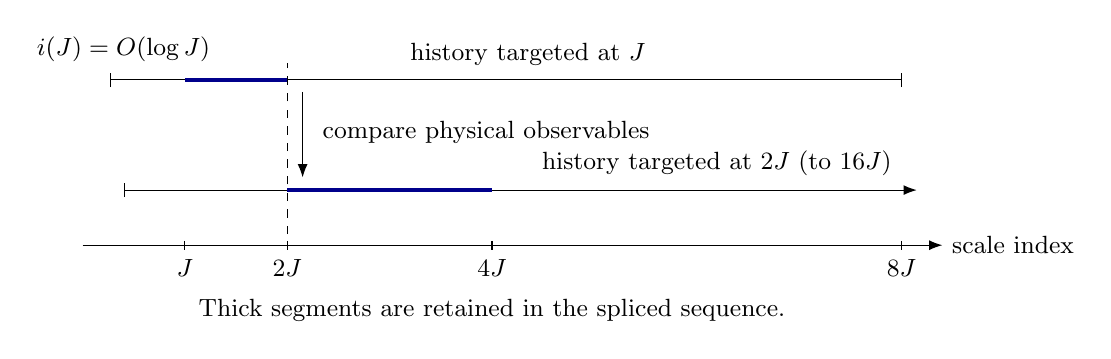
\begin{tikzpicture}[x=0.65cm,y=0.7cm,>=Latex,font=\small]
 \draw[->] (0,0)--(16.8,0) node[right] {scale index};
 \foreach \x/\lab in {2/J,4/2J,8/4J,16/8J}
  {\draw (\x,0.08)--(\x,-0.08) node[below] {$\lab$};}
 \draw[thin] (0.55,3)--(16,3);
 \draw[very thick,blue!55!black] (2,3)--(4,3);
 \draw (0.55,2.87)--(0.55,3.13);
 \draw (16,2.87)--(16,3.13);
 \node[above] at (0.8,3.15) {$i(J)=O(\log J)$};
 \node[above] at (8.7,3.08) {history targeted at $J$};
 \draw[thin,->] (0.82,1)--(16.3,1);
 \draw[very thick,blue!55!black] (4,1)--(8,1);
 \draw (0.82,0.87)--(0.82,1.13);
 \node[above left] at (16,1.08) {history targeted at $2J$ (to $16J$)};
 \draw[dashed] (4,0.2)--(4,3.3);
 \draw[->] (4.3,2.78)--(4.3,1.23);
 \node[right] at (4.5,2.05) {compare physical observables};
 \node[below,align=center] at (8,-0.8)
  {Thick segments are retained in the spliced sequence.};
\end{tikzpicture}
\caption{Finite histories overlap well beyond the intervals retained in
the spliced sequence. Coordinates are compared at the same absolute
scale using observables of the original height law. The picture is
schematic near the entry indices; no convergence rate at entry is
assumed.}
\label{fig:histories}
\end{figure}


We use the singleton and remainder coordinates from
Proposition~\ref{inp:balanced-map}.  The unbalanced coordinates are
$(t,z,\mathcal R)$: the first two multiply the gradient singleton
$e_B^0/2$ and the fundamental singleton $c_B^\alpha$, respectively.
The balanced gradient and fundamental coordinates are $(T,Z)$.
Parametrizing the exact Gaussian curves gives the coordinate $u$, and
subtracting the corresponding Gaussian remainder gives $B=B_e+B_o$,
where the subscripts denote the even and odd parts under translation
by $\pi/\alpha$.  In these coordinates an exact Gaussian trajectory
is $(u,0,0,0)$ with $u$ unchanged by the map.  The curve depends on its
entry index; the reference covariance kernels at a specified absolute
index do not.

\begin{lemma}[Uniform maps and the absolute coefficient estimates]
\label{lem:bulk-parity}
The coordinate changes and parity-resolved maps of
Proposition~\ref{inp:balanced-map} have a common analytic neighborhood
and common bounds for all sufficiently large entry indices $i(J)$.
At absolute index $k$, their two scalar quadratic coefficients obey
\begin{equation}\label{eq:bulk-coefficient-rate}
 H_k=H+O((1+k)^{-2}),\qquad
 b_k=b_*+O((1+k)^{-2}),\qquad
 H>0,\quad b_*=2\log L.
\end{equation}
The coefficients $H_k,b_k$ are independent of the entry index.
The constants in the parity remainder bounds are uniform in the
$J$-history.
\end{lemma}

\begin{proof}
The balanced projections are the convergent future linear projection
series in \cite[Equations (8.17) and
(8.18)]{B}.  Their norms and inverse norms are uniform
at every sufficiently large scale.  The covariance used here is the
nearest-neighbor polynomial covariance in the fixed absolute-index
convention.  Consequently its linear maps and future projection
series, and hence its balanced quadratic coefficients, are functions
of the absolute index alone.

We first check that parametrizing the Gaussian curves does not
introduce a dependence of the analytic radius on the entry scale.
At side $L^i$, initialize the exact partition algebra with the
exponential of $d\sum_B e_B^0/2$.  A fixed small complex disk in $d$
is permitted by the energy reserve in the entry regulator.  The
normalized block energy has the same bound at every entry scale.
For a smooth terminal source, Gaussian completion involves the
inverse of $I-dC^{1/2}AC^{1/2}$, where $C$ is the reference tail
covariance and $A$ is the unit-edge Laplacian.  Energy contraction
bounds this inverse uniformly on a fixed smaller disk.  The
gradient diagnostic and transverse contraction in
\cite[Lemma 10.3]{B} therefore bound all these
Gaussian trajectories and their analytic derivatives uniformly.
Smaller diagnostic tori cause no problem in this argument: the
Gaussian initialization has no entry sewing operations.  This is
also the uniformity argument used at the end of
\cite[Section 5]{X}.  The cosine decomposition
does not change it, since the pure Gaussian trajectory has zero
charged coordinates.  Its balanced gradient coordinate is
$T_k^g(d)=d+O(d^2)$, with uniform first derivative, and therefore
has an inverse on a common disk.  The transverse derivative of the
Gaussian remainder at $d=0$ is zero.  The parity estimates of
\cite[Lemma 10.6]{B} thus hold uniformly after this
change of coordinates.  The change leaves the $Z^2$ and $uZ$
coefficients unchanged.

The limits and signs in \eqref{eq:bulk-coefficient-rate}, with
$b_*=\alpha^2\log L/(4\pi)=2\log L$, follow from
\cite[Proposition 8.5 and Equation
(8.21)]{B}.  We need a rate in this particular
calculation.  We give the quantitative version of its finite-depth
approximation, since qualitative convergence of these coefficients
would not suffice below.

Truncate each future projection series at depth $r$.  Uniform
contraction of the linear remainder map makes the discarded part
at most $C\vartheta^r$ for some $\vartheta<1$.  Shell eigenvalue
errors and the kernel errors in fixed-order scaled differences are
power-small in $L^k$, by \cite[Lemma 8.1 and Equation
(8.9)]{B}.  We claim that replacing all kernels in
the retained depth-$r$ calculation by their continuum kernels has
error bounded by
\begin{equation}\label{eq:bulk-finite-depth-error}
 \exp\{C_L(1+r)^p\}L^{-ck}
\end{equation}
for fixed $p<\infty$ and $c>0$.

Indeed, a quadratic image starts with two singleton inputs and has
bounded support size.  Thereafter only linear maps occur.  A linear
continuation takes block closures, extracts a singleton, or
subtracts that extraction.  Support size consequently remains
bounded, and the number of shapes, routed blocks and extraction
choices through depth $r$ is at most
$C_L^{O((1+r)^2)}$.  Write singleton energies throughout in scaled
differences with their volume-normalized cell sums.  The original
two inputs have bounded polynomial degree.  Each subsequent Taylor
projection takes at most two derivatives on a constant or affine
background, with output a quadratic polynomial, a constant, or a
single phase harmonic.  With independent variables for the successive
Gaussian shells, the resulting Gaussian polynomial-character
expectations have at most $C_L(1+r)$ polynomial or derivative slots.
Their pairing expansions have at most factorial growth in this
number of slots.  Scale ratios and distances are bounded by
$C_L^{1+r}$.  The real character exponential has modulus at most
one; its change under kernel replacement can be estimated along
the line segment between two positive covariance matrices.  These
facts bound the expectation, and its derivative with respect to
any covariance entry, by the exponential factor in
\eqref{eq:bulk-finite-depth-error}.

Only values and fixed-order scaled differences of kernels enter
these slots.  Later Taylor projections differentiate the remaining
background field, not previously integrated kernels.  Converting
between the finitely many scales introduces at most
$C_L^{O((1+r)^2)}$.  The volume-normalized lattice sums satisfy the
same bound: couple each lattice sample to its mesh cube and use
one additional derivative of the smooth continuum shell kernel.
The block-shape sums are unchanged by this coupling.  This proves
\eqref{eq:bulk-finite-depth-error}; in particular it is a bound on
the explicit singleton calculation, not an assertion of uniform
Riemann approximation for arbitrary activities.

Choose $r=C_0\log(2+k)$.  A sufficiently large $C_0$ makes the
projection tail $O((1+k)^{-3})$, while
$\exp\{C_L(1+r)^p\}L^{-ck}=O((1+k)^{-3})$ for large $k$.
Weakening the bound gives \eqref{eq:bulk-coefficient-rate}.
\end{proof}

\subsection{Periodic physical diagnostics}

We now identify observables which test the two nearly marginal
coordinates.  Fix a sufficiently large dyadic $D_0$ and use tori of
side
\begin{equation}\label{eq:bulk-stopping-tori}
 N_k=D_0L^k.
\end{equation}
The constant $D_0$ exceeds the causal clearance of the local maps.
For each admissible stop, the torus has its own exact recursion from
the same entry scale as the plane history.  Its singleton coefficients
agree with the plane ones.  Its remainder need not agree with the
plane remainder and will be estimated separately.

Only stops with $N_k\ge sP$ are used.  Before this condition holds
there are at most $O(1+\log R)$ plane steps.  Their bounded map
amplification is $R^{O(1)}$, which is absorbed by the exponentially
small entry norm when $R$ is increased.  All stopping tori are
compatible with the observation and tile grids.

Let $f$ be the first real horizontal cosine on the unit torus, and
put
\begin{equation}\label{eq:bulk-test-definitions}
 g=(f,(-\Delta_{\mathbb T^2})^{-1}f)>0,\qquad
 X_N=(y,f_N),\qquad \chi_N=e^{i\bar y}.
\end{equation}
Here $f_N$ is sampled at observation-cell centers and includes the
cell-area weights, and $\bar y$ is the uniform mean of the
observations.  Heights are taken modulo a common translation by
$2\pi$, so $e^{i\bar h}$ is well defined.  The expectation in the
next lemma is for the periodic Bessel height law before inserting
the cutoff, together with its independent observation noises.

\begin{lemma}[The two physical limits]
\label{lem:bulk-physical-diagnostics}
As $N\to\infty$ with $s/N\to0$, locally uniformly for complex $w$,
\begin{align}
 \E e^{wX_N}&\longrightarrow e^{agw^2/2},
 \label{eq:bulk-physical-gradient}\\
 \E(\chi_Ne^{wX_N})-\E\chi_N\,e^{agw^2/2}
 &\longrightarrow0.
 \label{eq:bulk-physical-phase}
\end{align}
All fixed source derivatives converge as well.  For $s/N\le P^{-1}$,
the discrepancies can be made uniformly small by first increasing
$R$, hence $P$, and then increasing $s$.  The same statements hold
with the cutoff on every stopping torus of a $J$-history, uniformly
up to index $8J$.
\end{lemma}

\begin{proof}
We first transfer the height limit in
\cite[Theorem 2.4]{X} from free rectangles to
the periodic graph.  For a smooth periodic function $v$, test the
height by $(\partial h,\partial v_N)$.  Cut a fixed macroscopic
grid of seams to obtain free rectangles.  The retained tests depend
only on their internal gradients.  The centered comparison on the
independent Gaussian chains therefore bounds their variances and
real transforms by those on the cut graph.  There are $O(N)$ seam
edges, with test coefficients $O(N^{-1})$.  Their squared flow
cost is $O(N^{-1})$, so the omitted test tends to zero in reference
cost by \cite[Lemma 2.3]{X}.  The free
rectangle limits give the upper bound
$a\int|\nabla v|^2$ for each subsequential covariance limit.

For a function $v$ supported in a coordinate rectangle, choose a
pinning band outside its support and ground one representative
height at a point of the band.  Adding the hard pin decreases the
variance by the finite comparisons.  The mixed pinned limit in
\cite[Theorem 3.1]{X} gives the lower bound
$a\int|\nabla v|^2$, since $v$ is supported strictly inside the
pinning band.  Hence equality holds for such local functions.
The upper-bound defect of any subsequential covariance limit is
a positive semidefinite form.  A vector on which its quadratic
form vanishes belongs to its null space, by Cauchy--Schwarz for
positive semidefinite forms.  A smooth partition of unity writes
every periodic $v$ as a finite sum of these local functions.
Equality thus holds for every $v$, including their mixed
covariances.  The comparison argument is valid on the periodic
Gaussian-chain approximation at a fixed graph before passing to
the Bessel limit; no bare inverse-energy bound is transferred.

The corresponding Laplace limits follow by the same two comparisons.
For the lower bound, the centered variance comparison used in the
proof of \cite[Theorem 2.4]{X} supplies the
variance-based lower bound for the transform.  For the upper bound,
cut to the fixed grid of free rectangles and use their Laplace
limits.  H\"older's inequality separates the omitted seam term;
its reference cost tends to zero, and the H\"older exponent on
the retained term can then be sent to one.  Uniform exponential
bounds from \cite[Lemma 2.3]{X} give
convergence of every fixed moment and local uniform convergence
of the complex transforms.  Smooth mean-free density tests follow
by solving the periodic Poisson equation and approximating in
reference energy.  For the first cosine this also follows directly
from its discrete Laplacian eigenvalue.

Cell sampling changes the normalized reference standard deviation
of this test by $O(s/N)$, by the periodic Poincar\'e inequality
or the cell flow estimate.  Its observation-noise standard
deviation is also $O(s/N)$.  This proves
\eqref{eq:bulk-physical-gradient}, including its differentiated
version.

The phase requires more than the marginal Gaussian limit.  We
adapt the replica calculation of
\cite[Lemma 10.1]{B}.  Remove the
independent observation noise temporarily, and write $X_N^{(h)}$
for the height part of the cosine test.  We first work at one
fixed Gaussian-chain approximation of the size-$N$ graph.  The
pin selects a height representative and its law is invariant
under $h\mapsto-h$.  Let $h_1,h_2$ be independent copies on
the entire subdivided graph, including the chain variables, and put
\[
 S=h_1+h_2,\qquad \Delta=h_1-h_2.
\]
Their common coordinatewise parity class is
$\mathcal P=S\bmod4\pi\Z=\Delta\bmod4\pi\Z$.  If $Q$ denotes
the quadratic precision form, the change of variables gives
$Q(h_1)+Q(h_2)=(Q(S)+Q(\Delta))/2$.  Conditional on
$\mathcal P$, the fields $S,\Delta$ are consequently independent
and identically distributed.  Their conditional laws are centered:
each parity coset is preserved by sign reversal.  This is the
replica identity of \cite[Equation (2.12), in the
proof of Theorem 2.5]{X}.

For this fixed approximation write $X(h)$ for the cosine test and
$\mu(h)$ for the mean over the original sites, both extended as
linear forms on the subdivided field.  Thus $X(h)$ approximates
$X_N^{(h)}$ and $\mu(h)$ approximates $\bar h$.  Define the scalar
sum and difference tests and their conditional variance by
\begin{align*}
 A&=X(h_1)+X(h_2)=X(S),\\
 D&=X(h_1)-X(h_2)=X(\Delta),\\
 V&=\E(A^2\mid\mathcal P)=\E(D^2\mid\mathcal P).
\end{align*}
Put $\sigma^2=\E X(h)^2$ and
$\kappa_4=\E X(h)^4-3\sigma^4$.  Conditional independence gives
$\E V^2=\E(A^2D^2)$.  Since
$A^2D^2=(X(h_1)^2-X(h_2)^2)^2$, independence of the original
replicas yields $\E V^2=2\E X(h)^4-2\sigma^4$ and therefore
\begin{equation}\label{eq:bulk-replica-variance}
 \E V=2\sigma^2,\qquad \operatorname{Var}V=2\kappa_4.
\end{equation}

For real $t$ define the transform and the difference-character
\[
 F(t)=\E e^{i\mu(h)+itX(h)},\qquad
 \Psi_t= e^{i\mu(\Delta)+itX(\Delta)}.
\]
The character $\Psi_t$ depends only on the difference field and
has modulus one.  Conditional independence gives
$\E(A^2\Psi_t)=\E(V\Psi_t)$.  Inversion symmetry of the second
replica gives $\E\Psi_t=F(t)^2$.  The same sign reversal and
differentiation of $F$ give, with primes denoting $t$ derivatives,
\[
 \E(A^2\Psi_t)
 =(-F'')F+F(-F'')+2(-iF')(iF')
 =-2\bigl(FF''-(F')^2\bigr).
\]
We have thus proved the exact finite-approximation identity
\begin{equation}\label{eq:bulk-weighted-replica}
 -2\bigl(FF''-(F')^2\bigr)
 =2\sigma^2F^2+
   \E\bigl[(V-2\sigma^2)\Psi_t\bigr],
 \qquad t\in\R.
\end{equation}
Cauchy--Schwarz and \eqref{eq:bulk-replica-variance} bound its
last term by $\sqrt{2\kappa_4}$.

Take the chain limit first, at the fixed original graph.  The
fixed-graph moment convergence passes the second and fourth
moments, the transforms and their first two derivatives through
this limit.  Consequently, for
$F_N(t)=\E e^{i\bar h+itX_N^{(h)}}$ in the original Bessel law,
the absolute difference between the two sides of
\eqref{eq:bulk-weighted-replica} without its last term is at most
$\sqrt{2\kappa_{4,N}}$, where
$\kappa_{4,N}=\E(X_N^{(h)})^4-3(\E(X_N^{(h)})^2)^2$.
The Gaussian moment convergence proved above gives
$\kappa_{4,N}\to0$ and
$\operatorname{Var}(X_N^{(h)})\to ag$.
Uniform exponential bounds on compact complex sets permit
locally uniform subsequential limits of $F_N$ and all their
fixed derivatives.  For any such limit, denoted again by $F$,
\eqref{eq:bulk-weighted-replica} therefore implies on the real
axis, and then everywhere by analytic continuation,
\begin{equation}\label{eq:bulk-replica-ode}
 FF''-(F')^2=-agF^2.
\end{equation}
Half-wavelength translation preserves $e^{i\bar h}$ and changes
the sign of the cosine test.  Repinning after translation only
subtracts a height in $2\pi\Z$, so it leaves this phase unchanged.
Hence $F'(0)=0$.  If $F$ is not identically zero, solving the equation
where $F\ne0$ and then continuing analytically shows that $F$ is
an exponential quadratic without zeros.  Thus
$F(t)=F(0)e^{-agt^2/2}$.  The identically zero limit has the same
factorization.  Restoring the independent observation noise proves
\eqref{eq:bulk-physical-phase}.

These arguments also give the asserted order of choices.  Compare
the cell test to the ordinary sampled cosine with an error bounded
by $C/P$ when $s/N\le P^{-1}$.  First make this bound small, and
then use convergence of the ordinary cosine tests for all
$N\ge sP$.  Finally the cutoff error
\eqref{eq:cutoff-error}, including fixed exponential tests and
source derivatives, is bounded throughout a $J$-history by
\[
 C\exp\{C_LJ-cs_J\}=O(e^{-c'J^3}).
\]
Consequently it changes none of the preceding conclusions.
\end{proof}

We record the map interpretation of these tests.  A source $wX_N$
translates the remaining field by a smooth function $F$ satisfying
$B_s\alpha F$ equal to the reference observation covariance applied
to the source.  It can be chosen as a microscopic cosine: translation
symmetry makes the observation-cell function a cosine, and cell
averaging of the corresponding microscopic cosine has a multiplier
bounded away from zero.  Gaussian completion gives
\begin{equation}\label{eq:bulk-F-energy}
 (F,AF)=aw^2g+O_w((s/N)^c+N^{-c})
\end{equation}
for a fixed $c>0$, with uniform scaled derivatives in the point
norm.  One can obtain this error by periodic inverse-energy
approximation of the sampled density and the Taylor expansion of
the first discrete eigenvalue.

At a stop with $D_0^2$ blocks, the analytic terminal expansion of
\cite[Equations (10.3) and
(10.4)]{B} gives
\begin{align}
 \log\E e^{wX_N}-\log\E_a e^{wX_N}
 &=\tfrac12t_k(F,AF)
   +O(\norm{\mathcal R_k^{\rm tor}}+\nu_k^2),
 \label{eq:bulk-map-gradient}\\
 e^{-\log\E_a e^{wX_N}}\E(\chi_Ne^{wX_N})-\E\chi_N
 &=z_k\mathcal M_k(w)
   +O(\norm{\mathcal R_k^{\rm tor}}+\nu_k^2).
 \label{eq:bulk-map-phase}
\end{align}
Here $\nu_k=|t_k|+|z_k|+\norm{\mathcal R_k^{\rm tor}}$,
and $\E_a$ denotes the reference Gaussian observation law.  For
one fixed sufficiently small nonzero real $w$, both displayed
linear multipliers are bounded away from zero.  Explicitly the
second multiplier is
\begin{equation}\label{eq:bulk-phase-multiplier}
 \mathcal M_k(w)=\frac{D_0^2}{2}
 e^{\tau_k/2-\alpha^2D_{{\rm tail},k}/2}
 \operatorname{ave}_x(e^{-i\alpha F(x)}-1).
\end{equation}
The tail diagonal $D_{{\rm tail},k}$ is bounded, and the last
average tends to a strictly negative number for the fixed $w$.
The number $\tau_k$ is the variance, in observation units, of
the integrated Gaussian means.  It is bounded because the
zero-mode continuation at side $u$ contributes $O(u^2/N_k^2)$.
The compensating factor $e^{\tau_k/2}$ is necessary: insertion
of the retained uniform mean gives the physical mean-phase
insertion times $e^{-\tau_k/2}$.  This prescription is exact for
the cutoff interaction, which is periodic in the common mean.
Before tilt and subtraction, the same formula with spatial
factor one is a real positive multiplier bounded above and below.

\subsection{No exit and the nonexponential odd sector}

\begin{lemma}[Smallness on the finite horizons]
\label{lem:bulk-window-vanishing}
For every sufficiently small prescribed tube radius, the entry
parameters can be chosen so that all $J$-histories, for sufficiently
large $J$, remain in that tube through index $8J$.  The stopped
torus remainders remain in a fixed comparable tube.  Moreover,
for every fixed $0<c<8$,
\begin{equation}\label{eq:bulk-window-vanishing}
 \sup_{cJ\le k\le8J}
 \bigl(|u_k^{(J)}|+|Z_k^{(J)}|
       +\norm{B_{e,k}^{(J)}}+\norm{B_{o,k}^{(J)}}\bigr)
 \longrightarrow0.
\end{equation}
The analogous stopped torus remainder quantities tend to zero.
\end{lemma}

\begin{proof}
We use the two diagnostics exactly at the finite stops at which
they have just been justified.  Before a first candidate exit,
contraction of the plane remainder, and separately contraction of
the remainder on each stopping torus, give
\[
 \norm{\mathcal R_k},\ \norm{\mathcal R_k^{\rm tor}}
 \le C\vartheta^{k-i(J)}\varepsilon+C\rho^2.
\]
Here $\rho$ bounds the coordinates before the candidate exit,
$\varepsilon$ is the entry norm, and $\vartheta<1$.  Boundedness
of one map keeps the candidate state in a fixed multiple of that
tube.  Equations \eqref{eq:bulk-map-gradient} and
\eqref{eq:bulk-map-phase} and the nonzero multipliers bound its
singleton coordinates by
$C(\delta_{\rm diag}+\varepsilon+\rho^2)$, where
$\delta_{\rm diag}$ bounds the physical discrepancies.
Choose $\rho$ so that the quadratic term is smaller than a
fixed small multiple of $\rho$; next choose $R$ large and the
entry norm and diagnostic discrepancies small compared with
$\rho$.  Lemma~\ref{lem:bulk-physical-diagnostics} and
Proposition~\ref{prop:entry} permit these choices.  For large
$J$ the candidate cannot be an exit.  The finitely many initial
plane-only steps were controlled after
\eqref{eq:bulk-stopping-tori}.  The coordinate changes are
uniformly bounded by Lemma~\ref{lem:bulk-parity}, so this argument
applies to either coordinate system.

For the convergence assertion, take the supremum limiting plane
size over sequences with $J\to\infty$ and
$k-i(J)\to\infty$, $k\le8J$.  Call it $q_0$.  It lies in the
small tube, and all fixed numbers of preceding steps satisfy
the same limiting bound.  Iterating contraction over $r$ steps
and then sending $r\to\infty$ bounds the limiting plane
remainder by $Cq_0^2$.  The torus remainder has its own
contraction with the same plane singleton forcing, so the
same bound holds at its separate stops.  The test errors tend
to zero because $s/N_k\to0$ on these sequences.  The diagnostics
therefore give $q_0\le C'q_0^2$.  Taking the original tube
smaller than $1/C'$ implies $q_0=0$.  Every window in
\eqref{eq:bulk-window-vanishing} satisfies
$k-i(J)\to\infty$, which proves the stated uniform result.
\end{proof}

The preceding lemma gives convergence to the Gaussian fixed point.
To determine the approach rate we must also rule out exponential
decay in the odd direction.  The relevant lower bound is a
statement about the original periodic model at absolute side
$N_k$; it therefore does not depend on the entry history.

\begin{lemma}[Positive odd coordinate and contracted remainders]
\label{lem:bulk-odd}
On every fixed window $cJ\le k\le8J$, $0<c<8$, and for large
$J$, the period convention may be kept unchanged and
\begin{equation}\label{eq:bulk-odd-estimates}
 Z_k^{(J)}>0,\qquad -\log Z_k^{(J)}=o(J),\qquad
 \norm{B_{e,k}^{(J)}}\le C(Z_k^{(J)})^2,
 \qquad
 \norm{B_{o,k}^{(J)}}\le
 C\bigl(|u_k^{(J)}|+(Z_k^{(J)})^2\bigr)Z_k^{(J)}.
\end{equation}
The $o(J)$ and the constants are uniform on the window.
\end{lemma}

\begin{proof}
Let $Y_k=\E e^{i\bar h_{N_k}}$ for the original periodic height
law.  We first show
\begin{equation}\label{eq:bulk-phase-lower}
 Y_k>0,\qquad -\log Y_k=o(k).
\end{equation}
For free squares let $z_n^{\rm face}$ be the positive
characteristic ratio of the averaged four-face profile in
\cite[Equation (2.15)]{X}.  At $a=8\pi$ there is
$c_0>0$, independent of the fixed sufficiently large integer $r$,
such that
\[
 \liminf_{n\to\infty}
 \frac{z_{L^rn}^{\rm face}}{z_n^{\rm face}}\ge c_0.
\]
Replace $c_0$ by a smaller number in $(0,1)$.  For each fixed $r$,
iterate the eventual bound $c_0/2$ on the $r$ residue classes of
the absolute index.  This gives
\[
 \limsup_{k\to\infty}\frac{-\log z_{N_k}^{\rm face}}k
 \le\frac{\log(2/c_0)}r.
\]
Sending $r\to\infty$ proves subexponential decay of this free
characteristic.  The difference of the face profile and the
uniform profile has bounded reference cost.  The phase transfer
inequality \cite[Equation (2.2)]{X}, or its
application in \cite[Lemma 10.7]{B},
changes a logarithmic loss $o(k)$ by at most $O(1+\sqrt{o(k)})$.
Periodic edge restoration increases the positive characteristic
by \cite[Lemma 2.2]{X}.  This proves
\eqref{eq:bulk-phase-lower}.  Observation noise multiplies it
by $\exp\{-O((s/N_k)^2)\}$, and the cutoff changes it by
$O(e^{-cJ^3})$ on the windows under consideration.  Both changes
are negligible compared with \eqref{eq:bulk-phase-lower}.

Fix a slightly larger window starting at a smaller positive
fraction of $J$.  By Lemma~\ref{lem:bulk-window-vanishing} all
coordinates there tend uniformly to zero.  For a fixed small
$\epsilon>0$, consider the cone
\[
 \norm{B_o}\le\epsilon|Z|.
\]
The parity map makes it forward invariant once the window is
sufficiently late.  Indeed inside the cone its scalar equation
gives $|Z_+/Z-1|=o(1)$ uniformly, whereas its odd remainder
equation gives
$\norm{B_{o,+}}\le(\vartheta\epsilon+o(1))|Z|$.
In particular the sign of $Z$ cannot change inside the cone.

While the trajectory lies outside the cone,
$|Z|\le\epsilon^{-1}\norm{B_o}$; the odd remainder equation
then contracts $B_o$ with some factor $\vartheta'<1$.  It gives
the same geometric upper bound on $Z$ until the cone is entered.
This alternative cannot persist for a positive fraction of $J$.
To see this with the physical observable, the stopped mean-phase
expectation has an odd factor under the common-mean integral.
It is bounded by the plane odd singleton and the stopped torus
odd remainder.  The balance relations bound the unbalanced
plane odd variables by $|Z|+\norm{B_o}$.  The torus odd remainder
satisfies a geometric convolution of these plane odd inputs,
plus a geometric transient: every nonlinear odd-sector term
contains an odd factor.  An interval of length proportional to
$J$ outside the cone would therefore make the phase exponentially
small at its last stop, contradicting
\eqref{eq:bulk-phase-lower}.  Taking successively enlarged
windows gives cone entrance strictly before the desired window.

Inside the cone, the adjacent $|Z|$ ratios tend uniformly to one.
For any prescribed small $\delta>0$, the preceding convolution
is thus bounded by $C|Z_k|+Ce^{-cJ}$, since earlier inputs are
at most $(1+\delta)^r|Z_k|$ after $r$ backward steps and
$\vartheta(1+\delta)<1$.  Equation
\eqref{eq:bulk-phase-lower} consequently implies
$|Z_k|\ge e^{-o(J)}$ throughout the desired window.  In
particular all homogeneous contraction transients are negligible
relative to every fixed positive power of $|Z_k|$.

Iterate the even remainder equation with these adjacent ratio
bounds.  Its forcing is $O(Z^2)$, and the transient is negligible,
so $\norm{B_{e,k}}\le C Z_k^2$.  The scalar equation then gives
$|u_{k+1}-u_k|\le CZ_k^2$.  For $r$ steps backward within an
enlarged window,
\begin{equation}\label{eq:bulk-backward-u}
 |Z_{k-r}|\le(1+\delta)^r|Z_k|,\qquad
 |u_{k-r}|\le |u_k|+Cr(1+\delta)^{2r}Z_k^2.
\end{equation}
Using these bounds in the odd contraction gives
\[
 \norm{B_{o,k}}
 \le C\sum_{r\ge0}\vartheta^r
 (|u_k|+C(1+r)(1+\delta)^{2r}Z_k^2)
 (1+\delta)^r|Z_k|
 \le C(|u_k|+Z_k^2)|Z_k|,
\]
where $\delta$ is chosen so that
$\vartheta(1+\delta)^3<1$.  The finitely truncated convolution
has only a negligible transient.  This proves the norm bounds.

Finally the untilted mean-phase expansion, with its positive
linear multiplier described after
\eqref{eq:bulk-phase-multiplier}, is
$M_kZ_k+o(|Z_k|)+O(e^{-cJ})$, where $M_k$ is bounded positively
above and below.  The torus odd remainder has the sharper bound
just obtained by the same contraction argument.  The physical
phase is positive by \eqref{eq:bulk-phase-lower}, and its
cutoff error is negligible.  Thus $Z_k>0$ in the unchanged period
convention.  Since the coordinates also tend to zero, the
lower bound $Z_k\ge e^{-o(J)}$ is exactly the logarithmic
assertion in \eqref{eq:bulk-odd-estimates}.
\end{proof}

\subsection{Readouts common to different entry scales}

The estimates obtained so far do not yet identify a single
trajectory: each $J$-history uses different observation cells and
different cutoffs.  We now compare their coordinates using
observables of the same original periodic model.

Let $\widetilde X_{N_k}$ be the ordinary microscopic sampled cosine,
without observation averaging or noise, and define
\begin{equation}\label{eq:bulk-common-observables}
 U_k=\frac{\operatorname{Var}(\widetilde X_{N_k})}{g},
 \qquad Y_k=\E e^{i\bar h_{N_k}}.
\end{equation}
Both quantities depend only on the absolute index $k$.

\begin{proposition}[Common readouts]
\label{prop:bulk-readouts}
For every $0<c<8$, uniformly on $cJ\le k\le8J$,
\begin{align}
 U_k&=\frac{a}{1-u_k^{(J)}}+O((Z_k^{(J)})^2)+O(e^{-c'J}),
 \label{eq:bulk-U-readout}\\
 Y_k&=M_kZ_k^{(J)}
 +O\bigl((|u_k^{(J)}|+(Z_k^{(J)})^2)Z_k^{(J)}\bigr)
 +O(e^{-c'J}).
 \label{eq:bulk-Y-readout}
\end{align}
Here $c'>0$ may depend on $c$, and $M_k$ is bounded above and
below by positive constants and is common to all histories,
up to an exponentially small error which is included in the
display.  The coordinate changes also give
\begin{equation}\label{eq:bulk-coordinate-conversion}
 t_k=u_k+O(u_k^2+Z_k^2),\qquad
 z_k=\ell_k^{-1}Z_k+O((|u_k|+Z_k^2)Z_k),\qquad
 \norm{\mathcal R_k}\le C(u_k^2+Z_k^2),
\end{equation}
where $\ell_k$ is the absolute-index fundamental balancing
factor and is bounded above and below positively.
\end{proposition}

\begin{proof}
At step $k$ compare the plane activity with the exact Gaussian
trajectory having parameter $d=u_k$.  The even balanced remainder
has size $O(Z_k^2)$ by Lemma~\ref{lem:bulk-odd}; the odd remainder
has size $O((|u_k|+Z_k^2)Z_k)$.  Undoing the linear balance,
using its parity, gives a difference $O(Z_k^2)$ in the gradient
coordinate and
\begin{equation}\label{eq:bulk-z-conversion}
 z_k=\ell_k^{-1}Z_k+O((|u_k|+Z_k^2)Z_k).
\end{equation}
The Gaussian remainder is $O(u_k^2)$.  These facts prove
\eqref{eq:bulk-coordinate-conversion}.

The stopped torus requires a separate comparison, since its
remainder need not copy the plane.  Run its own exact map from
entry, comparing at intermediate index $r$ with its Gaussian
trajectory at parameter $u_r$.  Gaussian torus trajectories
and their first parameter derivatives are bounded uniformly:
this follows from the same energy completion and contraction
argument as Lemma~\ref{lem:bulk-parity}.  Changing the comparison
parameter from $u_r$ to $u_{r+1}$ costs $O(Z_r^2)$ by
\eqref{eq:bulk-backward-u}.  The remainder forcing has zero
linear singleton derivative at zero.  First the odd torus
contraction gives $O(Z_r)$.  Its even forcing from odd inputs
is then $O(Z_r^2)$.  Comparing even components with the Gaussian
curve and iterating contraction gives $O(Z_r^2)$ in the even
difference.  Returning to the odd equation improves its forcing
to $O((|u_r|+Z_r^2)|Z_r|)$: pure odd terms beyond linear have
at least three odd factors, and every other such term has an
even factor of size $O(|u_r|+Z_r^2)$.  The adjacent-ratio bounds
and \eqref{eq:bulk-backward-u} justify the same geometric
convolutions as in Lemma~\ref{lem:bulk-odd}.  Initial transients
are $O(e^{-c'J})$ on the stated window.

All terminal integrations are analytic on a uniform neighborhood,
with a fixed number $D_0^2$ of blocks and regulator reserve.
In the variance diagnostic a term odd under half-period shift
has zero first derivative at the Gaussian trajectory.  Hence
the difference from that trajectory is $O(Z_k^2)+O(e^{-c'J})$.
It remains to compute the Gaussian value in the coordinate $u$,
rather than approximate a Gaussian trajectory in activity norm.

Hold its initial parameter $d$ fixed.  Let $C_i$ be the reference
tail covariance at the entry side $L^i$.  Direct completion of
the initial quadratic exponential gives, beyond the reference
source prefactor, the log transform
\begin{equation}\label{eq:bulk-Gaussian-readout}
 \frac d2
 \bigl(A^{1/2}F,
 (I-dA^{1/2}C_iA^{1/2})^{-1}A^{1/2}F\bigr).
\end{equation}
On the first mode the operator $A^{1/2}C_iA^{1/2}$ has eigenvalue
$1+O((L^i/N_k)^2)$, by the low-pass polynomial formula.
Together with \eqref{eq:bulk-F-energy}, two source derivatives
therefore give normalized variance
$a/(1-d)+O((L^i/N_k)^c+(s/N_k)^c+N_k^{-c})$.
On a fixed positive-fraction window these errors are
$O(e^{-c'J})$.  Set $d=u_k$ and compare the cell test to the
original sampled cosine in reference energy.  Removing its
noise and cutoff has the same error.  This proves
\eqref{eq:bulk-U-readout}.

For the mean-phase diagnostic the purely even terms integrate
to zero.  Expanding in the odd difference from the Gaussian
trajectory, using \eqref{eq:bulk-z-conversion} and the odd
remainder bound, gives \eqref{eq:bulk-Y-readout}.  The
coefficient at zero activity is the untilted terminal
fundamental multiplier times $\ell_k^{-1}$.  It is real positive
and uniformly bounded above and below.  Finally we verify its
independence from the history.  Its high-mean variance includes
all Gaussian shells below the stop, including those integrated
at entry below $L^{i(J)}$.  These variances telescope to the
same absolute-index sum for every entry choice.  The remaining
tail variance and $\ell_k$ also depend only on $k$.
Observation noise contributes only $O((s/N_k)^2)$ to the
exponent.  Thus a single sequence $M_k$ can be used in
\eqref{eq:bulk-Y-readout}, absorbing the exponentially small
noise correction into its error.  The cutoff removal is again
exponentially smaller still.
\end{proof}

We have proved three facts about every long interior window of a
finite history: its state tends to zero, its odd coordinate is
positive and only subexponentially small, and its two scalar
coordinates can be read from physical observables independent of
entry.  These are the inputs for the trajectory argument that
follows.

\section{Joining finite histories and determining the critical trajectory}
\label{sec:trajectory}

The bulk estimates provide a small trajectory on each finite scale
window.  The histories have different entry scales, so they need not
agree as activity families on their overlaps.  Their physical readouts
nevertheless determine the two marginal coordinates accurately enough
to compare them.  We first use those comparisons to form one infinite
sequence, and then determine its leading coefficient.  The coefficient
of the gradient activity obtained at the end of this section is the
one needed in the magnetic terminal calculation.

\subsection{An abstract lemma for sparse changes of history}

An ordinary evolution step increases the scale index by one.  A change
of history takes place at a fixed scale index and does not count as an
additional evolution step.  The following notation keeps these two
operations distinct.  We write $(u_j,Z_j)$ for the state used to start
the ordinary step at index $j$, and
$(\widetilde u_{j+1},\widetilde Z_{j+1})$ for the output of that step.
At an index where no change of history occurs, the tilded state is
$(u_{j+1},Z_{j+1})$.  At a change of history, it is the state immediately
before the change.

\begin{lemma}[A trajectory with geometrically separated jumps]
\label{lem:trajectory-sparse-splice}
Let $H,b>0$, let $j_0\ge1$, and let $\mathcal Q$ be a set of integers
larger than $j_0$.  Suppose that the increasing enumeration $(q_r)$ of
$\mathcal Q$ satisfies
\[
 q_{r+1}\ge \rho q_r
 \qquad\text{for some fixed }\rho>1.
\]
The set $\mathcal Q$ may also be finite or empty.  For every integer
$j\ge j_0$, let $(u_j,Z_j)$ and
$(\widetilde u_{j+1},\widetilde Z_{j+1})$ be real states with positive
second coordinates.  Assume that both coordinates of every state tend
to zero as its scale index tends to infinity.  Suppose that the
ordinary evolution satisfies
\begin{align}
 \widetilde u_{j+1}-u_j
   &=-H_j Z_j^2
       +O\bigl((|u_j|+Z_j^2)Z_j^2\bigr),
       \label{eq:trajectory-ordinary-u}\\
 \frac{\widetilde Z_{j+1}}{Z_j}
   &=1-b_j u_j+O(u_j^2+Z_j^2),
       \label{eq:trajectory-ordinary-z}\\
 H_j&=H+O(j^{-2}),\qquad b_j=b+O(j^{-2}).
       \label{eq:trajectory-coefficients}
\end{align}
For $q>j_0$ with $q\notin\mathcal Q$, assume
$(u_q,Z_q)=(\widetilde u_q,\widetilde Z_q)$.  At every $q\in\mathcal Q$,
assume instead
\begin{align}
 |u_q-\widetilde u_q|&\le C\widetilde Z_q^2,
       \label{eq:trajectory-jump-u}\\
 |Z_q-\widetilde Z_q|
   &\le C\bigl(|\widetilde u_q|+\widetilde Z_q^2\bigr)
                  \widetilde Z_q.
       \label{eq:trajectory-jump-z}
\end{align}
All constants in these hypotheses are uniform in the scale index.
Then, with $x_*=(H/b)^{1/2}$,
\begin{align}
 \frac{u_j}{Z_j}&=x_*+O(j^{-1}),
       \label{eq:trajectory-ratio}\\
 \frac1{Z_j}&=b x_*j+O(\log j),
       \label{eq:trajectory-inverse}\\
 u_j&=\frac1{bj}+O\left(\frac{\log j}{j^2}\right),\qquad
 Z_j=\frac1{\sqrt{bH}\,j}
                 +O\left(\frac{\log j}{j^2}\right).
       \label{eq:trajectory-asymptotics}
\end{align}
The same estimates hold for the states immediately before jumps.
\end{lemma}

\begin{proof}
We first obtain positive, comparable coordinates without assuming a
rate of convergence.  We then derive the rate $j^{-1}$, and finally
identify its coefficient by solving the equation for $u/Z$ backwards.

\paragraph{Grouping a jump with preceding evolution.}
Fix an integer $K$, whose size will be chosen below.  Discard finitely
many initial indices so that the intervals $[q-K,q]$, $q\in\mathcal Q$,
are disjoint.  This is possible because the gaps between consecutive
elements of $\mathcal Q$ tend to infinity.  Replace the $K$ ordinary
steps from $q-K$ to the state immediately before $q$, together with
the jump at $q$, by one grouped transition.  Retain every other
ordinary step.  Thus consecutive retained indices have difference
either $1$ or $K$.  A grouped transition of length $K$ still contains
exactly $K$ ordinary evolution steps.

Write $(u,Z)$ for the state at the beginning of such a transition.
For fixed $K$, induction in the ordinary recurrence gives, at each
of its intermediate ordinary states,
\[
 Z_{\mathrm{int}}/Z=1+o(1),\qquad
 u_{\mathrm{int}}=u+O_K(Z^2).
\]
The errors are uniform along the tail.  More precisely, immediately
before the jump the $K$ ordinary steps give
\begin{align}
 \widetilde u_q-u
   &=-KHZ^2+O_K\bigl((|u|+Z^2+j^{-2})Z^2\bigr),
       \label{eq:trajectory-k-u}\\
 \widetilde Z_q/Z
   &=1-Kbu+O_K(u^2+Z^2+j^{-2}|u|),
       \label{eq:trajectory-k-z}
\end{align}
where $j=q-K$.  To see these estimates, use the first recurrence to
bound the change in $u$ by $O_K(Z^2)$, and substitute this bound in the
second recurrence.  Multiplying its $K$ ratios creates only terms
bounded by $O_K(u^2+Z^2)$.  Substitution back into the first recurrence
then gives \eqref{eq:trajectory-k-u}.

The jump changes the right side of \eqref{eq:trajectory-k-u} by at
most $(C+o(1))Z^2$.  Its contribution to
\eqref{eq:trajectory-k-z} has absolute value at most
$(C+o(1))|u|+O_K(Z^2)$.  Here the leading constant $C$ is a constant
from the jump hypotheses, independent of $K$; the terms caused by
$\widetilde u_q-u$ are included in $O_K(Z^2)$.  Any error bounded by
$C_1|u|+C_KZ^2$ can be written as a coefficient of $u$, of absolute
value at most $C_1$, plus an $O_K(Z^2)$ term.  This remains true at
$u=0$, when the first term is zero.

Choose $K$ sufficiently large compared with the jump constants and
with $H^{-1},b^{-1}$.  After moving farther along the tail, every
retained transition therefore satisfies
\begin{equation}
 u^+-u=-\alpha Z^2,\qquad
 \frac{Z^+}{Z}=1-\beta u+r,
 \qquad |r|\le C_K Z^2,
 \label{eq:trajectory-grouped}
\end{equation}
where
\begin{equation}
 0<\alpha_-\le\alpha\le\alpha_+<\infty,
 \qquad
 0<\beta_-\le\beta\le\beta_+<\infty.
 \label{eq:trajectory-grouped-bounds}
\end{equation}
The bounds also hold for a retained single ordinary step.  The
coefficients $\alpha,\beta$ may vary from one transition to another;
no regularity of that dependence is used.

\paragraph{Positivity and the two comparison cones.}
At retained nodes, $u$ strictly decreases, because $Z>0$.  Its limit
is zero by hypothesis, so $u>0$ at every node of this tail.  We next
show that this positive coordinate is comparable to $Z$.

Choose $c_->0$ so small that $c_-^2\beta_+<\alpha_-/2$.
Whenever $u\le c_-Z$, \eqref{eq:trajectory-grouped} gives
\[
 (u^+-c_-Z^+)-(u-c_-Z)
   =-\alpha Z^2+c_-\beta uZ-c_-rZ
   \le -\tfrac14\alpha_-Z^2
\]
on a sufficiently late tail.  Consequently the region
$u-c_-Z\le0$ is forward invariant, and once it is entered the
quantity $u-c_-Z$ becomes strictly negative and then decreases.
This contradicts its convergence to zero.  Thus $u>c_-Z$.

Choose $c_+>0$ so large that
$c_+^2\beta_->2\alpha_+$.  Whenever $u\ge c_+Z$, the same computation
gives
\[
 (u^+-c_+Z^+)-(u-c_+Z)
   =-\alpha Z^2+c_+\beta uZ-c_+rZ
   \ge hZ^2
\]
for some $h>0$ on a sufficiently late tail.  This region is also
forward invariant.  Entry would make $u-c_+Z$ strictly positive and
increasing, again contradicting convergence to zero.  We have proved
\begin{equation}
 c_-Z<u<c_+Z
 \label{eq:trajectory-cones}
\end{equation}
at all sufficiently late retained nodes.

\paragraph{The first rate estimate.}
Put $x=u/Z$ at a retained node.  From
\eqref{eq:trajectory-grouped} and \eqref{eq:trajectory-cones},
\[
 \frac1{Z^+}-\frac1Z
   =\frac{\beta u-r}{Z(1-\beta u+r)}
   =\beta x+O(Z).
\]
This increment is bounded above and bounded away from zero.  Its
sum is therefore comparable to the number of retained transitions.
The physical scale index increases by either $1$ or $K$ at each
such transition, so that number is comparable to the scale index.
It follows that $Z\asymp j^{-1}$ and $u\asymp j^{-1}$ at retained
nodes.  The intermediate estimates preceding
\eqref{eq:trajectory-k-u}, together with the jump bounds, extend
these comparisons to every ordinary state and every state before a
jump.  In particular,
\begin{equation}
 Z_j\asymp j^{-1},\qquad u_j\asymp j^{-1},\qquad
 0<c\le u_j/Z_j\le C,
 \label{eq:trajectory-first-rate}
\end{equation}
and the corresponding tilded bounds hold as well.

We now know the order of both coordinates.  The remainder of the
proof identifies their leading coefficient.  For this purpose we
return to the original ordinary steps and keep each jump as a
separate event at its actual scale index.

\paragraph{Backward determination of the ratio.}
For an ordinary step, division of
\eqref{eq:trajectory-ordinary-u} by
\eqref{eq:trajectory-ordinary-z}, using
\eqref{eq:trajectory-first-rate}, gives
\begin{align}
 \frac{\widetilde u_{j+1}}{\widetilde Z_{j+1}}
          -\frac{u_j}{Z_j}
   &=(b x_j^2-H)Z_j+O(j^{-2})\notag\\
   &=b(x_j+x_*)(x_j-x_*)Z_j+O(j^{-2}),
 \qquad x_j=\frac{u_j}{Z_j}.
 \label{eq:trajectory-ratio-step}
\end{align}
At a jump, direct division and
\eqref{eq:trajectory-jump-u}--\eqref{eq:trajectory-jump-z} yield
\begin{equation}
 \left|\frac{u_q}{Z_q}
            -\frac{\widetilde u_q}{\widetilde Z_q}\right|
       \le Cq^{-1}.
 \label{eq:trajectory-ratio-jump}
\end{equation}

List all ordinary steps and all jumps in their chronological order,
and put $y=x-x_*$ at every state in this list.  An ordinary step
has the form
\[
 y^+=(1+a)y+e,\qquad
 a=b(x+x_*)Z,\qquad c/j\le a\le C/j,
 \qquad |e|\le Cj^{-2}.
\]
A jump has the same form with $a=0$ and $|e|\le C/q$.
For two positions $s<t$ in this event list, let $P_{s,t}$ be the
product of the factors $1+a$ between them.  The factors are at least
one, and $P_{s,t}\to\infty$ as $t\to\infty$ for fixed $s$, because
there is one ordinary step at every integer scale and
$\sum_jj^{-1}=\infty$.  Iterating the equation and solving for the
earlier value gives
\[
 y_s=\frac{y_t}{P_{s,t}}
       -\sum_{r=s}^{t-1}\frac{e_r}{P_{s,r+1}}.
\]
The values $y_t$ are bounded by \eqref{eq:trajectory-first-rate}.
Letting $t\to\infty$, and bounding the denominators below by one,
therefore shows, for a state at scale $j$,
\[
 |y_s|\le
 C\sum_{k\ge j}k^{-2}
   +C\sum_{\substack{q\in\mathcal Q\\q\ge j}}q^{-1}
 \le \frac Cj.
\]
The last bound uses geometric separation: if $q$ is the first jump
at or after $j$, the remaining reciprocals sum to at most
$q^{-1}/(1-\rho^{-1})$.  This proves
\eqref{eq:trajectory-ratio} at every state, including those before
jumps.

\paragraph{Counting ordinary time.}
For an ordinary step we now have
\begin{align*}
 \frac1{\widetilde Z_{j+1}}-\frac1{Z_j}
   &=b_j\frac{u_j}{Z_j}+O(j^{-1})
     =b x_*+O(j^{-1}).
\end{align*}
At a jump, \eqref{eq:trajectory-jump-z} and
\eqref{eq:trajectory-first-rate} give
\[
 \left|\frac1{Z_q}-\frac1{\widetilde Z_q}\right|\le C.
\]
There are $O(\log j)$ jumps up to scale $j$.  Telescoping from a
fixed initial index to $j$ counts exactly one ordinary increment
for each increase of the scale index by one.  The sum of the
ordinary errors is $O(\log j)$, and the sum of jump errors has the
same bound.  Hence \eqref{eq:trajectory-inverse} holds.  Inverting
that estimate and using \eqref{eq:trajectory-ratio} proves
\eqref{eq:trajectory-asymptotics}, since
$x_*/(b x_*)=1/b$.  A final jump changes $u$ and $Z$ by $O(j^{-2})$,
so these conclusions also hold for the states before jumps.
\end{proof}

\subsection{Application to the bulk histories}

For a dyadic integer $J$, attach a superscript $(J)$ to the
coordinates of the history whose entry index is $i(J)$ and whose
last index is $8J$.  The entry estimate gives $i(J)=O(\log J)$.
Thus, for every fixed $c>0$, the interval $[cJ,8J]$ lies after entry
when $J$ is large.  The estimates below are uniform on such intervals,
with constants allowed to depend on $c$.

\begin{lemma}[Comparison at a common scale]
\label{lem:trajectory-overlap}
Consider two bulk histories with comparable window parameters $J,J'$.
At an index $j$ belonging to fixed positive-fraction windows of both
histories, write $(u,Z)$ and $(u',Z')$ for their balanced marginal
coordinates.  For all sufficiently large indices,
\begin{equation}
 |u'-u|\le CZ^2,
 \qquad
 |Z'-Z|\le C(|u|+Z^2)Z.
 \label{eq:trajectory-overlap}
\end{equation}
The constants are uniform when the comparison factors for the two
windows are fixed.
\end{lemma}

\begin{proof}
The two readouts in Proposition~\ref{prop:bulk-readouts} concern the
same microscopic observables at scale $j$.  Consequently their values
can be written using either history as
\begin{align*}
 U_j&=\frac a{1-u}+O(Z^2)+O(e^{-c_0\min(J,J')}),\\
 Y_j&=M_jZ+O\bigl((|u|+Z^2)Z\bigr)
                   +O(e^{-c_0\min(J,J')}),
\end{align*}
and likewise with primes.  Here $a>0$ is fixed, and $M_j$ is common
to the two histories and bounded above and below by positive
constants.  An exponentially small discrepancy in $M_j$ can be
included in the displayed error.

By Lemmas~\ref{lem:bulk-window-vanishing} and
\ref{lem:bulk-odd}, the coordinates tend uniformly to zero,
$Z,Z'>0$, and $-\log Z,-\log Z'=o(\min(J,J'))$.  The exponential
errors are therefore negligible relative to every fixed positive
power of either $Z$ or $Z'$.  The second readout first implies
$Z'\asymp Z$: its error relative to its own leading term tends to
zero on each history.  Comparing the first readout now gives
\[
 \left|\frac a{1-u'}-\frac a{1-u}\right|\le CZ^2.
\]
The derivative of $a/(1-u)$ is bounded below positively near zero,
so $|u'-u|\le CZ^2$.  Substitute this estimate and $Z'\asymp Z$
back into the second readout.  After division by the positive lower
bound on $M_j$, it gives the second bound in
\eqref{eq:trajectory-overlap}.
\end{proof}

\begin{proposition}[The bulk trajectory throughout an overlap window]
\label{prop:bulk-window}
Fix the block factor $L$ and the other parameters chosen for the
bulk maps.  For every sufficiently large dyadic $J$, uniformly in
the $J$-history at integer indices $J/2\le j\le3J$, its unbalanced
gradient coordinate $t_j$, fundamental coordinate $z_j$, and plane
remainder $\mathcal R_j$ satisfy
\begin{equation}
 t_j=\frac1{2j\log L}
                 +O\left(\frac{\log j}{j^2}\right),
 \qquad |z_j|=O(j^{-1}),
 \qquad \|\mathcal R_j\|=O(j^{-2}).
 \label{eq:trajectory-bulk-window}
\end{equation}
The remainder norm is the unbalanced plane activity norm.
\end{proposition}

\begin{proof}
Select a dyadic $J_0$ large enough for the preceding estimates, and
use the $J$-history on $J\le j<2J$, for
$J=J_0,2J_0,4J_0,\ldots$.  At the index $2J$, first evolve the
$J$-history through its ordinary step from $2J-1$ to $2J$.  Regard
that output as the state before the change, and then replace it by
the state of the $2J$-history at the same index.  Both states lie in
the available positive-fraction windows.  Lemma~\ref{lem:trajectory-overlap}
gives \eqref{eq:trajectory-jump-u}--\eqref{eq:trajectory-jump-z} for
this replacement.

Lemma~\ref{lem:bulk-window-vanishing} makes all selected states and
all states before changes tend to zero.  Lemma~\ref{lem:bulk-odd}
provides $Z>0$ and the balanced remainder estimates
\[
 \|B_{e,j}\|\le CZ_j^2,
 \qquad
 \|B_{o,j}\|\le C(|u_j|+Z_j^2)Z_j.
\]
Inserting them into the bulk recurrences, with the parity structure
of Lemma~\ref{lem:bulk-parity}, gives
\eqref{eq:trajectory-ordinary-u}--\eqref{eq:trajectory-coefficients}
with
\[
 H>0,\qquad b=2\log L.
\]
The jumps occur at $2J_0,4J_0,8J_0,\ldots$, so they satisfy the
geometric-separation hypothesis with $\rho=2$.
Lemma~\ref{lem:trajectory-sparse-splice} consequently gives on the
selected path
\begin{equation}
 u_j=\frac1{2j\log L}
          +O\left(\frac{\log j}{j^2}\right),
 \qquad Z_j=O(j^{-1}),
 \qquad \|B_{e,j}\|=O(j^{-2}),
 \qquad \|B_{o,j}\|=O(j^{-2}).
 \label{eq:trajectory-balanced-window}
\end{equation}
The displayed odd bound is sufficient here; its stated forcing
estimate in fact gives $O(j^{-2})$ directly from $u_j,Z_j=O(j^{-1})$.

These estimates must also hold on histories not selected at a given
index.  Fix a $J$-history and $J/2\le j\le3J$.  Let $J'$ be the
dyadic parameter selected at $j$, so $J'\le j<2J'$.  Then $J$ and
$J'$ are comparable, and $j$ belongs to fixed positive-fraction
windows of both histories.  Apply
Lemma~\ref{lem:trajectory-overlap} with the selected state as the
unprimed state.  Since that state has $u,Z=O(j^{-1})$, the two
$u$ coordinates differ by $O(j^{-2})$, and so do the two $Z$
coordinates.  Lemma~\ref{lem:bulk-odd} then gives the same remainder
bounds on the $J$-history.  Thus
\eqref{eq:trajectory-balanced-window} holds throughout every
window asserted in the proposition, with uniform constants.

Finally undo the balance transformations and the subtraction of the
analytic Gaussian curve used to define $u,B_e,B_o$.  The coordinate
relations in \eqref{eq:bulk-coordinate-conversion} give
\begin{align*}
 t&=u+O(u^2+Z^2),\qquad |z|\le C|Z|,\\
 \|\mathcal R\|
   &\le C\bigl(u^2+Z^2+\|B_e\|+\|B_o\|\bigr).
\end{align*}
The quadratic order in the last line includes the remainder of the
Gaussian curve, whose constant and linear gradient terms have
already been separated.  Applying these relations to
\eqref{eq:trajectory-balanced-window} proves
\eqref{eq:trajectory-bulk-window}.
\end{proof}

The argument uses uniform convergence on positive-fraction windows
and the common physical readouts with their stated nonlinear errors.
The additional errors from entry-scale smoothing
and cutoff removal are exponentially small on those windows.
No rate of convergence in the height scaling limit was used to
obtain the coefficient $1/(2\log L)$.

\section{The magnetic recursion in two squares}\label{sec:magnetic}

The bulk trajectory controls activities far from the boundary and the
source.  We now extend that control to the free walls and the magnetic
mark.  The purpose of the extension is to compare two squares using
exactly the same scalar normalization at the mark.  The insertion at
entry can have a polynomially large norm; its residual part will
contract, while its extracted scalar will cancel in the comparison.

Fix a large integer $j$, put $M=L^j$, and consider the free dual
squares of sides $Q=M$ and $Q=LM$, with their common center at the
mark.  Choose the $J$-history of Proposition~\ref{prop:bulk-window},
where $J$ is a power of two and $J\le j<2J$.  Its entry scale is
$m=L^i=qRs$, with $s\asymp_L J^3$ and $i=O(\log J)$.
In both squares stop at the same scale
\begin{equation}\label{eq:mag-common-stop}
 v=L^h,\qquad
 j-h=\left\lceil\log_L(j^{1/10})\right\rceil,
 \qquad D=\frac{M}{v}.
\end{equation}
Thus $j^{1/10}\le D<Lj^{1/10}$ and $M/(Ps)\to\infty$.
In particular the entry footprint and every fixed number of blocks
about the mark fit strictly inside both squares at all scales used.

We use the blocks, compatibility relation, analytic activity norms,
and covariance shells of the preceding sections.  Write
$\mathscr Z_k(K;\phi)$ for the subset partition functional at scale
$L^k$: it sums products of the activities $K(X;\phi)$ over compatible
collections of nonempty connected supports, including the empty
collection.  Thus $\mathscr Z_k$ is the functional
$\mathcal Z_{L^k}$ of Section~\ref{sec:inputs}, indexed here by its
absolute scale.  For another activity family $I$, define
\begin{equation}\label{eq:mag-first-variation}
 \mathscr I_k(K,I;\phi)
 =\left.\frac{d}{d\varepsilon}
       \mathscr Z_k(K+\varepsilon I;\phi)\right|_{\varepsilon=0}.
\end{equation}
Each term on the right has exactly one $I$ factor; the original
exclusions between that factor and the background factors are
retained.  The entry representation of Proposition~\ref{prop:entry}
has this form in the pierced square: in its notation,
$\mathscr I_i(K,I;\phi)=\mathcal Z_m^{(1)}(K,I;\phi)$.

For every support $X$ at scale $L^k$, let $\operatorname{Rect}_k(X)$ be its
axis-parallel spanning rectangle, and let $\operatorname{Rect}_k^H(X)$ be
that rectangle enlarged by $HL^k$ in each coordinate direction.
In a square, call $X$ \emph{bulk-good} if $\operatorname{Rect}_k^H(X)$ lies
strictly inside the square, and a \emph{wall support} otherwise.
Independently, call $X$ \emph{shift-good} if
$\operatorname{Rect}_k^H(X)$ misses the mark, and a \emph{defect support}
otherwise.  These predicates apply to supports of every size; they
specify both the full wall and defect norms below and the terminal
support decomposition.

The constant $H$ is fixed before $L$, independently of the entry
box parameter $P$.  It is large enough for the testing and assignment
radii and for the geometric sum of predecessor-dependence radii
used in copying.  The same definition at an output scale uses
$H$ \emph{coarse} blocks.  It does not require a bulk-good fine
input to be clear of its entire shell, whose range can be of order
$L$ fine blocks.  The entry convention for unused background supports
inside the compulsory footprint allows $H$ to remain independent
of $P$.

Figure~\ref{fig:common-core} shows the geometry of the common stop.
The local computations determining the marked scalars take place in
the same interior region; the wall contributions remain in the
terminal activities.
\begin{figure}[tb]
\centering
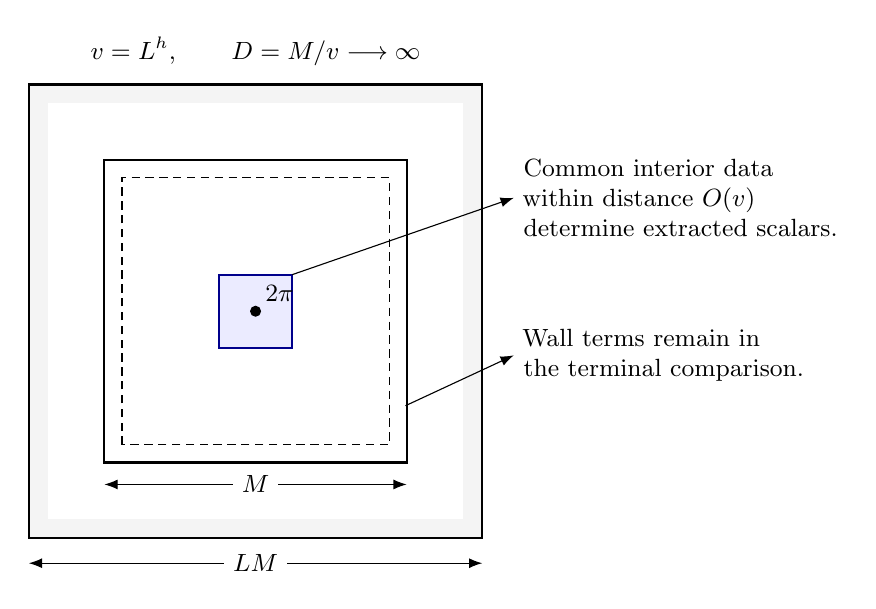
\begin{tikzpicture}[x=0.8cm,y=0.8cm,>=Latex,font=\small]
 \fill[gray!9] (-3.6,-3.6) rectangle (3.6,3.6);
 \fill[white] (-3.3,-3.3) rectangle (3.3,3.3);
 \draw[thick] (-3.6,-3.6) rectangle (3.6,3.6);
 \draw[thick] (-2.4,-2.4) rectangle (2.4,2.4);
 \draw[densely dashed] (-2.12,-2.12) rectangle (2.12,2.12);
 \fill[blue!8] (-0.58,-0.58) rectangle (0.58,0.58);
 \draw[blue!55!black,thick] (-0.58,-0.58) rectangle (0.58,0.58);
 \fill (0,0) circle (2pt);
 \node[above right] at (0,0) {$2\pi$};
 \draw[->] (0.58,0.58)--(4.1,1.8);
 \node[right,align=left,text width=4cm] at (4.1,1.8)
  {Common interior data\\within distance $O(v)$\\determine extracted scalars.};
 \draw[->] (2.38,-1.5)--(4.1,-0.7);
 \node[right,align=left,text width=4cm] at (4.1,-0.7)
  {Wall terms remain in\\the terminal comparison.};
 \draw[<->] (-2.4,-2.75)--(2.4,-2.75)
  node[midway,fill=white] {$M$};
 \draw[<->] (-3.6,-4)--(3.6,-4)
  node[midway,fill=white] {$LM$};
 \node[above] at (0,3.75) {$v=L^h,\qquad D=M/v\longrightarrow\infty$};
\end{tikzpicture}
\caption{Two concentric dual squares are stopped at the same block side
\(v\). The marked scalar computations use identical interior data,
whereas the remaining backgrounds are compared by terminal integration.
The common interior region has radius \(O(v)\), much smaller than \(M\).
The squares and collars are schematic and not drawn to scale.}
\label{fig:common-core}
\end{figure}


Let $K^0_{k,Q}$ and $K^l_{k,Q}$ denote the ordinary and pierced
background activities.  On a shift-good support the local lift
$\lambda_Q$ satisfies
$\partial\lambda_Q=\eta_l/\alpha$ and is defined up to a constant
multiple of the field period.  On interior supports meeting the
mark, the comparison with the pierced plane calculation instead
uses the smooth field
\[
 \gamma_Q=(r_Q-r_\infty)/\alpha.
\]
The lift estimates and entry copying established earlier apply in
these field units.

\begin{proposition}[Common magnetic normalization]\label{prop:magnetic}
For all sufficiently large $j$, the exact maps from entry scale $i$
to stop $h$ can be chosen with the following properties.
\begin{enumerate}
\item At the stop, in the fixed norm regimes for the ordinary and
defect activities,
\begin{equation}\label{eq:mag-small-backgrounds}
 \max_{Q\in\{M,LM\}}
 \bigl(\norm{K^0_{h,Q}}+\norm{K^l_{h,Q}}\bigr)\le \frac{C}{j}.
\end{equation}
The bulk copies satisfy the sharper conclusion of
Proposition~\ref{prop:bulk-window}.  On shift-good supports, pierced
activities are exactly ordinary activities evaluated at the local
lift.  Interior pierced activities copy the plane calculation at
the translate $\gamma_Q$, whenever their required clearance holds.

\item Let $a^\nu_{k,Q,b}$ be the designated scalar coefficient at
coarse block $b$ in step $k$, for $\nu=0,l$, and set
\begin{equation}\label{eq:mag-background-products}
 P^\nu_Q=\prod_{k=i}^{h-1}\prod_b(1+a^\nu_{k,Q,b}).
\end{equation}
All factors are real and positive.  The ratios agree exactly:
\begin{equation}\label{eq:mag-common-background-ratio}
 \frac{P^l_M}{P^0_M}=\frac{P^l_{LM}}{P^0_{LM}}=:\rho_j.
\end{equation}
For every fixed $\epsilon_2>0$, the initial smallness choices can
be made so that $|\log\rho_j|\le\epsilon_2j$ for all sufficiently
large $j$.

\item There are a real scalar $\sigma_Q$ and residual insertion
activities $I_{h,Q}$ such that integration of the entry insertion
over all shells below $v$ gives the exact field identity
\begin{equation}\label{eq:mag-insertion-identity}
 \E_{i:h}\mathscr I_i(K^l_{i,Q},I_{i,Q};\phi)
 =P^l_Q\left\{
    \sigma_Q\mathscr Z_h(K^l_{h,Q};\phi)
       +\mathscr I_h(K^l_{h,Q},I_{h,Q};\phi)\right\}.
\end{equation}
Here $\E_{i:h}$ denotes successive shell integration, with the
remaining field $\phi$ held fixed.  The scalar is common to the
two squares,
\begin{equation}\label{eq:mag-common-insertion-scalar}
 \sigma_M=\sigma_{LM}=: \sigma_j,
\end{equation}
and every support of $I_{h,Q}$ contains the designated mark block.
Moreover,
\begin{equation}\label{eq:mag-insertion-bound}
 \norm{I_{h,Q}}\le C_Rs^{C_R}L^{-2(h-i)/3},
 \qquad Q\in\{M,LM\}.
\end{equation}
\end{enumerate}
The products in \eqref{eq:mag-background-products} contain only
the RG extraction factors.  They do not include the common entry
scalar or the harmonic-energy factor of the Gaussian sector law.
\end{proposition}

We prove the proposition in four steps.  The localizations and
placement estimates are those of the exact partition map in
\cite[Section 4]{B}.  The wall and lifted-copy
constructions follow the method of its Propositions
5.5 and 5.7.  Their
low-temperature conclusions are not inputs here: the marginal
charge estimate, critical forcing, and insertion contraction needed
for the present proposition are established below.

\subsection{The wall estimate at the marginal frequency}

A small support means one in the small linear-input class of the
partition map.  Its fine-block size is bounded by the fixed
threshold $n_0$, and its coarse closure has index diameter at most
one.  In an ordinary square use the plane localization, including
the fundamental harmonic localization, on small bulk-good inputs.
On small wall inputs extract only the neutral constant.  Since a
small support has bounded diameter, the latter inputs lie within
a fixed number of fine-block layers of a wall.  A small bulk-good
input still uses the plane prescription if its shell convolution
can see the wall; its contribution to a wall output is treated as
forcing.  In contrast, the $H$ coarse-block clearance of a bulk-good
output ensures that every predecessor needed for copying lies in
the interior with its required shell and numerical dependence.

Ordinary activities are even in the field.  After neutral constant
subtraction, the localization lemma of
\cite[Lemma 4.5]{B} gives a factor $CL^{-2}$
for a small wall input.  There are $O_H(L)$ fine placements at a
prescribed coarse block along a wall, and only $O_H(1)$ at a
corner.  It remains to check the charged part at
$\alpha^2=8\pi$.

Let $\Gamma$ be the shell covariance from side $m'$ to side $Lm'$,
and let $x$ lie on a small wall support.  The binary kernel
estimates, with even reflection at a free wall, give
\begin{equation}\label{eq:mag-wall-shell}
 \Gamma(x,x)\ge\frac{\log L}{2\pi}-C,
 \qquad
 \norm{\Gamma(\,\cdot\,,x)-\Gamma(x,x)}_{m',X}\le C.
\end{equation}
Both constants are independent of $L$ after the geometric radii
are fixed.  For the diagonal estimate, the direct image supplies
the plane value.  An image contribution vanishes at binary scales
smaller than a fixed multiple of its separation, by finite range.
At scales larger than a sufficiently large fixed multiple of that
separation it is nonnegative: the positive plane binary diagonal
and the derivative estimate give this assertion.  Only boundedly
many intermediate binary scales can contribute negatively, and
each is bounded.  At a corner the same argument applies to the
finite set of reflected images.  Other walls are beyond the shell
range in the applications where this description is used.
Positive-order binary estimates summed over the shell prove the
second bound in \eqref{eq:mag-wall-shell}.

Apply the charge-contour estimate of
\cite[Equations (4.26) and
(8.14)]{B}, with shift amplitude
$a=\alpha$.  For nonzero integer charge $q$, its exponential gain
is bounded by
\[
 C\exp\{-\alpha^2(|q|-1/2)\Gamma(x,x)+h_0\alpha|q|\}.
\]
Using \eqref{eq:mag-wall-shell}, the fundamental charges have gain
$CL^{-2}$, and the higher charges form a summable series with
stronger powers of $L^{-1}$.  The analytic radius $h_0$ is chosen
before $L$ to allow the fixed nonconstant imaginary shift.  The
observation regulator is admissible in this estimate by
\cite[Lemma 9.2]{B} and its free-square version
verified at entry.  Thus the charged wall terms have the same
$CL^{-2}$ bound required for the placement count.

Let $p_k$ be the full ordinary plane activity norm, and let $w_k$
be the full norm restricted to ordinary wall supports as defined
above, without a small-size restriction.  Large linear inputs
have arbitrarily strong weight contraction after the activity
weight is chosen sufficiently large.  The analytic nonlinear
bound of the partition map and the preceding small-input estimates
give
\begin{equation}\label{eq:mag-wall-recursion}
 w_{k+1}\le\theta_1w_k+C_Lp_k+C_L(w_k+p_k)^2,
 \qquad \theta_1<1.
\end{equation}
Here $C_Lp_k$ includes plane inputs and assigned pieces that reach
a wall output.  Their field evaluations occur on their original
fine blocks with the prescribed collars, so no wall cancellation
is needed to bound them.  All norm regimes, including their
regulator reserves, are fixed once; the wall contraction does not
consume another reserve at each step.

\subsection{Defect localization and exact copying}

On a small shift-good input in the pierced square, use exactly
the localization pieces of its ordinary counterpart, evaluated at
the lifted field.  Designate exactly the same scalar for
extraction.  In particular a translated quadratic may have a
nonzero value at zero field, but that value remains part of the
quadratic piece; it is not extracted as an additional scalar.

For a small defect input $F_Q$, let
\[
 (F_Q)_0(\phi)=\frac{\alpha}{2\pi}
       \int_0^{2\pi/\alpha}F_Q(\phi+t)\,dt
\]
be its neutral projection.  In the plane extract
$\E(F_\infty)_0(\zeta)$, where $\zeta$ is the current shell.
In the square extract instead
\begin{equation}\label{eq:mag-backtranslated-extraction}
 c_Q(F_Q)=\E(F_Q)_0(\zeta-\gamma_Q).
\end{equation}
The neutral projection is invariant under constant field shifts,
so the alignment constant in $\gamma_Q$ does not affect this
definition.  Every small defect input is interior: its bounded
fine-block diameter and its failure to be shift-good place it
within $O_H(L^k)$ of the mark, while $L^k\le v/L=M/(DL)$ for
every input to a step before the stop.

The changed subtraction has the same contraction as ordinary
neutral constant subtraction.  Indeed the latter gives $CL^{-1}$
without evenness.  On a small fine support at side $m'=L^k$, the
nonconstant part of $\gamma_Q$ has fine test norm at most
$Cm'/Q$.  By the analytic derivative bound with its fixed
regulator reserve,
\begin{equation}\label{eq:mag-extraction-change}
 \left|c_Q(F_Q)-\E(F_Q)_0(\zeta)\right|
 \le C\frac{m'}{Q}\norm{F_Q}
 \le \frac{C}{L}\norm{F_Q}.
\end{equation}
The last inequality holds uniformly through the chosen stop for
large $j$.  Charged small defect inputs have gain $CL^{-2}$ by the
same contour argument, now with the interior shell estimates.
At a prescribed output there are only $O_H(1)$ small fine defect
placements.  Consequently their total residual norm is at most
$CL^{-1}$ times their input norm.

Translations of shift-good inputs use the norm reserves fixed at
entry.  On the relevant fine collars,
$m'|\nabla\lambda_Q|$ and $(m')^2|\nabla^2\lambda_Q|$ are bounded.
The quadratic inequality therefore permits a fixed increase in
the ordinary regulator exponent, and a fixed increase in the
coefficient of the variational observation regulator.  Each costs
at most $C^{|X|}$ on a support $X$, absorbed by the reserved activity
weight.  A localized piece that is assigned to a coarse singleton
is still evaluated on the fine block where its lift is defined.
This applies to both gradient pieces and fundamental harmonics;
a deterministic real phase does not enlarge the analytic norm of
the latter.  Thus pieces reaching defect outputs have controlled
norm without evaluating a lift at the singular core.

Let $d_k$ be the full defect norm, in this fixed reserved regime.
The same multilinear partition-map estimates as for the wall,
with the large-input weight gain in the defect norm, give
\begin{equation}\label{eq:mag-defect-recursion}
 d_{k+1}\le\theta_1d_k+C_L(p_k+w_k)
             +C_L(d_k+w_k+p_k)^2,
 \qquad\theta_1<1.
\end{equation}
The forcing term includes the translated ordinary pieces just
described.  This proves the analytic estimate needed near the mark.
We next verify the numerical equality that will make its scalar
normalization disappear between the two squares.

Suppose an output support has the stated clearance.  Every fine
input, assigned singleton piece, and scalar normalization entering
that output then fits in its enlarged neighborhood.  On a
shift-good output they share a common lift.  Products and Gaussian
convolution commute with this deterministic translation, and the
identical localizations preserve the translated-copy identity.
For an interior defect output use instead
\begin{equation}\label{eq:mag-pierced-copy}
 F_Q(\phi)=F_\infty(\phi+\gamma_Q).
\end{equation}
The shell kernels agree there by finite range, and
\eqref{eq:mag-backtranslated-extraction} gives the exact equality
\[
 c_Q(F_Q)=\E(F_\infty)_0(\zeta).
\]
It follows inductively that both activities and designated
coefficients copy the corresponding plane calculation.

This induction includes numerical, as well as field, dependence.
In the exact map, predecessor dependence from relocation and
singleton normalizers extends by at most a fixed multiple of the
current scale.  Over earlier steps these distances sum to a
geometric series.  The link construction at entry records any
numerical dependence reaching a wall in its support, so the same
argument starts at entry.  Enlarging $H$ by a fixed amount pays
these causal radii.  A support that still reaches a wall cannot
become a small marked input before the stop: the distance from
the mark to the wall, in stop blocks, tends to infinity.  Large
inputs do not supply scalar extractions.  Thus neither a long
entry link nor a large insertion support can introduce a hidden
wall dependence into the local constants at the mark.

The only differences between pierced and ordinary designated
constants arise from small defect inputs, so they occur at
$O_H(1)$ blocks per step.  At each of these blocks both the
pierced and ordinary constants are the same plane constants in
the two squares.  All other factors cancel in the
pierced-to-ordinary product within each square.  This proves
\eqref{eq:mag-common-background-ratio} exactly.

\subsection{Scalar extraction with one insertion}

For clarity, we record the scalar algebra before estimating the
insertion.  Write one exact background map as
\begin{equation}\label{eq:mag-one-map}
 \E\mathscr Z_k(K;\phi+\zeta)
   =p_k(K)\mathscr Z_{k+1}(\mathcal F_k(K);\phi),
 \qquad
 p_k(K)=\prod_b(1+a_{k,b}(K)).
\end{equation}
Here the $a_{k,b}$ are the designated coefficients of small linear
inputs.  Extend the same exact splitting algebra to coefficients in
$\R[\varepsilon]/(\varepsilon^2)$.  Its degree-zero terms use the
background localization; its degree-one terms use the marked
localization and allocation specified below.  Write
\[
 a_{k,b}(\varepsilon)=a_{k,b}+\varepsilon a'_{k,b},
 \qquad K_+=\mathcal F_k(K),\qquad
 K_+(\varepsilon)=K_++\varepsilon\mathcal T_k(K)I.
\]
Thus $\mathcal T_k(K)$ is the linear map in the insertion slot of
this extended construction.  It need not be the derivative of the
unmarked map $\mathcal F_k$, since the two slots have different
localization prescriptions.  Put
\[
 I_+=\mathcal T_k(K)I,
 \qquad
 \beta_k=\sum_b\frac{a'_{k,b}}{1+a_{k,b}}.
\]
The coefficient of $\varepsilon$ in the exact identity is
\begin{equation}\label{eq:mag-differentiated-map}
 \E\mathscr I_k(K,I;\phi+\zeta)
 =p_k(K)\left\{\beta_k\mathscr Z_{k+1}(K_+;\phi)
                    +\mathscr I_{k+1}(K_+,I_+;\phi)\right\}.
\end{equation}
This is differentiation of the partition identity with the stated
degree-dependent splittings.  No finite nonzero perturbation by the
possibly large $I$ is required.

If an earlier step has already produced a scalar $\sigma$, linearity
applied to $\sigma\mathscr Z_k(K)+\mathscr I_k(K,I)$ gives
\begin{equation}\label{eq:mag-scalar-recursion}
 \sigma_+=\sigma+\beta_k,
 \qquad I_+=\mathcal T_k(K)I.
\end{equation}
In particular the earlier scalar is kept outside the later map.
It is not put back into the activity as $\sigma K$.
This elementary identity is important because $\sigma$ need not
be small, whereas the operator controlling $I_+$ only sees the
small background $K$.

We also specify how the mark is preserved in the exact algebra.
Use \eqref{eq:mag-backtranslated-extraction} for small insertion
inputs, and assign their extracted constant to the coarse block
containing the designated fine mark block.  This assignment lies
in their coarse closure, as required by the partition map.  A
residual input keeps its closure label, including the mark.
In the scalar normalization step the decoration at block $b$ is
\[
 d_b=(1+a_b)^{-1}-1,
 \qquad d'_b=-\frac{a'_b}{(1+a_b)^2}.
\]
Only a small marked input can give $a'_b\ne0$, and its designated
block is the mark block.  Hence a differentiated decoration is
also supported at the mark.  Every term in a differentiated
product contains either an insertion input or such a decoration;
its final connected support therefore contains the mark.  Original
exclusions remain attached to relocated pieces, exactly as in
\cite[Proposition 4.8]{B}.  The differentiation
does not turn a compatible collection into an unrestricted product.

At zero background, the complete residual insertion map after
scalar extraction is the subtracted small linear map together
with the unchanged large linear map.  The small-input bound just
proved is $C/L$, with boundedly many marked placements.  By
increasing the large-support weight after fixing $L$, its remaining
linear contribution is as small as desired.  The multilinear bounds
for the exact partition map give
$\norm{\mathcal T_k(K)-\mathcal T_k(0)}\le C_L\norm{K}$ on the
fixed small background ball, and hence
\begin{equation}\label{eq:mag-insertion-operator}
 \norm{I_+}
 \le\left(\frac{C}{L}+\delta_A
                       +C_L\norm{K}\right)\norm{I},
\end{equation}
where $\delta_A$ tends to zero as the weight is increased.
For this degree-one map the background and insertion may have
different designated localizations: the exact splitting algebra
is linear in each input, and its multilinear estimates use the
same bounds on these designated pieces.  Thus
\eqref{eq:mag-insertion-operator} applies to the prescribed marked
splitting as well.  It imposes no smallness assumption on
$\norm{I}$ itself.

Choose $L$ so that $C/L<\tfrac13L^{-2/3}$, the weight so that
$\delta_A<\tfrac13L^{-2/3}$, and then the background tube so that
$C_L\norm{K}<\tfrac13L^{-2/3}$ at every step.  Iteration and the
entry insertion bound give \eqref{eq:mag-insertion-bound}.

Finally every summand in $\beta_k$ depends only on a small marked
input and the background normalizer at its assigned block.
The copying argument in the preceding subsection makes both its
numerator and denominator identical in the two squares.  This
also holds for the insertion activities by induction through
\eqref{eq:mag-differentiated-map}.  At entry the compulsory footprint
fits with clearance in both squares; a support too small to
contain it has insertion coefficient zero in both.  Starting with
$\sigma_i=0$, Equation~\eqref{eq:mag-scalar-recursion} therefore
gives $\sigma_M=\sigma_{LM}$.  This equality does not require a
bound or a sign for the accumulated scalar.

\subsection{Completion of the background bounds}

\begin{proof}[Proof of Proposition~\ref{prop:magnetic}]
The constructions above give the exact identities and the copying
assertions.  We complete the uniform estimates and the parameter
choices.  Fix the kernel and assignment radii, the clearance $H$,
and the finite list of norm regimes with their translation and
integration reserves.  Choose $L$ and then the activity weights
as in the local estimates.  The constants in the small-support
bounds before placement counting are independent of $L$.
After these choices take the bulk diagnostic tube sufficiently
small.  Proposition~\ref{prop:entry} supplies arbitrarily small
entry backgrounds in all of these fixed regimes, and the bulk
analysis keeps the plane activities in the prescribed tube.

The two recursions \eqref{eq:mag-wall-recursion} and
\eqref{eq:mag-defect-recursion} now keep the wall and defect
backgrounds small throughout the history.  More explicitly, by
decreasing the tube the quadratic terms can be absorbed into a
slightly larger contraction $\theta_2<1$ and a constant multiple
of their forcing terms.  Iteration first for $w_k$ and then for
$d_k$ proves the assertion.  On the last positive-fraction window,
Proposition~\ref{prop:bulk-window} gives $p_k\le C/j$.
The geometric convolutions in the two recursions therefore give
$w_h+d_h\le C/j$; the earlier part of each convolution is
exponentially small in $j$.  This proves
\eqref{eq:mag-small-backgrounds}, including its uniformity for
$Q=M$ and $Q=LM$.

All coefficients and localizations are real.  Their scalar
coefficients are bounded by a fixed map constant times the small
background tube, so $|a^\nu_{k,Q,b}|<1/2$ and every extracted
factor is positive.  Only boundedly many factors per step differ
between the pierced and ordinary maps.  Since
\[
 |\log(1+a)-\log(1+a')|\le2|a-a'|
 \qquad (|a|,|a'|<1/2),
\]
their cumulative ratio has logarithm at most $\epsilon_2j$ in
absolute value after the tube is decreased in terms of the
prescribed $\epsilon_2$.  This decrease is made after the fixed map
constants and remains compatible with the preceding choices.

The same smallness gives the insertion operator bound chosen
after \eqref{eq:mag-insertion-operator}.  Iterating
\eqref{eq:mag-differentiated-map}, keeping the scalar outside each
subsequent map as in \eqref{eq:mag-scalar-recursion}, proves
\eqref{eq:mag-insertion-identity}.  The equality of its scalar
between the two squares and the norm bound have already been
established.  This proves all parts of the proposition.
\end{proof}

\section{Terminal integration and the normalization constant}
\label{sec:terminal}

We now compare two squares using the same finite history.  The comparison
removes all scalar contributions from the microscopic magnetic core.
What remains is a deterministic energy difference and a small terminal
partition function.  The accuracy of the latter comparison, rather than
an estimate on the core amplitude, will give a convergent normalization.

Let $M=L^j$, $n=M/2$, and use the history with $J\leq j<2J$ as in
Proposition~\ref{prop:magnetic}.  For $Q\in\{M,LM\}$, the subscript $Q$
will indicate the free dual square of side $Q$.  Both calculations stop
at the scale in \eqref{eq:mag-common-stop}:
\begin{equation}
 v=L^h,\qquad
 j-h=\left\lceil\log_L(j^{1/10})\right\rceil,
 \qquad D=M/v.
 \label{eq:terminal-stop}
\end{equation}
In particular,
\begin{equation}
 j^{1/10}\leq D<Lj^{1/10},\qquad
 h=j-O_L(\log j).
 \label{eq:terminal-stop-size}
\end{equation}
There are $O_L(D^2)$ terminal blocks in either square.  All constants
below may depend on the parameters fixed before choosing the history,
including $L$, but not on $j$.

Write $\E_{*,Q}$ for expectation under the remaining reference Gaussian
field in the square of side $Q$, together with its common constant,
which is uniform modulo $2\pi/\alpha$.  Recall that $\alpha^2=8\pi$.
For $\varepsilon\in\{0,l\}$, define
\[
 \mathcal Z_Q^\varepsilon
 =\E_{*,Q}\mathscr Z_h(K^\varepsilon_{h,Q};\psi),
 \qquad
 \mathcal J_Q
 =\E_{*,Q}\mathscr I_h(K^l_{h,Q},I_{h,Q};\psi).
\]
Here $\mathscr Z_h$ is the compatible-support partition polynomial,
and $\mathscr I_h$ is its part with exactly one marked activity, as in
Proposition~\ref{prop:magnetic}.  In particular, $\mathcal J_Q$ does not
include the separately extracted scalar $\sigma_Q$.

\subsection{Uniform terminal integration}

The fact that $D$ grows is useful: it separates the magnetic core from
the wall at the terminal scale.  It also requires a terminal estimate
whose constants do not depend on the total number of blocks.

\begin{lemma}[Terminal partition expansion]
\label{lem:terminal-partition}
For the backgrounds of Proposition~\ref{prop:magnetic},
\begin{align}
 \mathcal Z_Q^\varepsilon&=1+O_L(D^2/j),
 \label{eq:terminal-partition-small}\\
 \log\mathcal Z_Q^\varepsilon
 &=\sum_X\E_{*,Q}K^\varepsilon_{h,Q}(X;\psi)
       +O_L(D^4/j^2).
 \label{eq:terminal-log}
\end{align}
They are real and positive for all sufficiently large $j$.  Moreover,
\begin{equation}
 |\mathcal J_Q|
 \leq C_LD^2\|I_{h,Q}\|.
 \label{eq:terminal-insertion}
\end{equation}
These estimates hold with the fixed regulator and activity-weight
reserves used in the magnetic construction.
\end{lemma}

\begin{proof}
The terminal regulator estimate in Proposition~\ref{inp:regulator} gives
\begin{equation}
 \E_{*,Q}\prod_{a=1}^p\mathcal G_h(X_a;\psi)
 \leq C^{|X_1|+\cdots+|X_p|}
 \label{eq:terminal-regulator}
\end{equation}
for compatible supports, with any one of the fixed reserved regulators
$\mathcal G_h$ used here.  The constant in this bound is independent of
$Q/v$.  To recall why the terminal estimate has this uniformity, the
positive-order differences of the remaining covariance are bounded at
scale $v$, and its energy form is bounded by the full reference form.
The blockwise Gaussian quadratic estimates in the regulator proof
therefore have uniformly bounded operator norm and trace proportional
to the number of blocks being tested.  Their exponential moments cost
at most $C^{|X|}$ on a support $X$.  Neither estimate uses an upper
bound on the number of blocks in the entire square.  Regulator
composition and monotonicity apply the same estimate to the union of
compatible supports.  The common constant causes no additional cost,
since the activities are periodic and the regulators depend only on
nonconstant fields.  These are the terminal bounds of
\cite[Sections 9 and 4]{B}; their
kernel hypotheses hold equally at the earlier stop
\eqref{eq:terminal-stop}.

Proposition~\ref{prop:magnetic} bounds each background by $C/j$ in the
activity norm.  Sum first over supports through a specified anchor
block and then over the $O_L(D^2)$ anchors.  The exponential cost in
\eqref{eq:terminal-regulator} is absorbed by the reserved activity
weight.  It follows that the absolute sum of terms of degree $p$ in
the terminal partition polynomial is bounded by
\[
                    (C_LD^2/j)^p.
\]
Since $D^2/j\to0$, the terms of degree at least two have total size
$O_L(D^4/j^2)$.  The constant term is one and the degree-one term is
the sum in \eqref{eq:terminal-log}.  This proves
\eqref{eq:terminal-partition-small}; expanding $\log(1+x)$ proves
\eqref{eq:terminal-log}.  Reality follows from the real-coefficient
construction, and closeness to one then gives positivity.  The same
calculation with one distinguished marked factor bounds the sum by
\[
 C_LD^2\|I_{h,Q}\|
       \sum_{p\geq0}(C_LD^2/j)^p.
\]
Absorbing this convergent series proves
\eqref{eq:terminal-insertion}.
\end{proof}

\subsection{Cancellation of the magnetic scalar}

Let $\widehat a_{Q/2}$ denote the ratio with the observation cutoffs
used for this history.  This notation depends on the chosen history;
only the two squares under simultaneous comparison use it below.
Set
\[
 E_Q=\|\eta_{l,Q}\|^2,
 \qquad H_Q=\exp\{-E_Q/(2\alpha^2)\}.
\]
The common preparation scalar cancels between the two sectors.  The
exact identities \eqref{eq:mag-background-products} and
\eqref{eq:mag-insertion-identity} therefore give
\begin{equation}
 \widehat a_{Q/2}
 =H_Q\rho_j
       \frac{\sigma_j\mathcal Z_Q^l+\mathcal J_Q}
            {\mathcal Z_Q^0},
 \qquad
 \rho_j=\frac{P_Q^l}{P_Q^0}>0.
 \label{eq:terminal-exact-ratio}
\end{equation}
Both $\rho_j$ and $\sigma_j$ are exactly the same for $Q=M$ and $Q=LM$.
The equality of $\sigma_j$ is algebraic; its sign has not been assumed.

\begin{lemma}[Relative removal of the residual insertion]
\label{lem:terminal-scalar}
There is $c>0$ such that, for all sufficiently large $j$,
$\sigma_j>0$ and
\begin{equation}
 \log a_{Q/2}
 =-\frac{E_Q}{2\alpha^2}+\log\rho_j+\log\sigma_j
    +\log\mathcal Z_Q^l-\log\mathcal Z_Q^0+O(e^{-cj})
 \label{eq:terminal-log-ratio}
\end{equation}
for both $Q=M$ and $Q=LM$.
\end{lemma}

\begin{proof}
The bounds on $s$, the entry index $i$, and the terminal index $h$ give
$s=O_L(j^3)$, $i=O_L(\log j)$, and $j-h=O_L(\log j)$.  By
\eqref{eq:mag-insertion-bound} and
\eqref{eq:terminal-insertion}, the marked term in the physical ratio
\eqref{eq:terminal-exact-ratio} is bounded by
\begin{equation}
 \left|H_Q\rho_j\frac{\mathcal J_Q}{\mathcal Z_Q^0}\right|
 \leq \operatorname{poly}(j)L^{-2j/3}e^{\epsilon_2j}.
 \label{eq:terminal-physical-residual}
\end{equation}
Here $H_Q\leq1$, the denominator is bounded below by
Lemma~\ref{lem:terminal-partition}, and
Proposition~\ref{prop:magnetic} gives
$|\log\rho_j|\leq\epsilon_2j$.  The positive number $\epsilon_2$ may
be chosen arbitrarily small by shrinking the background tube after
fixing the map constants.  Choose $\epsilon_2<(\log L)/6$.

Lemma~\ref{inp:regular-variation} gives
$a_{Q/2}\geq c_L L^{-j/2}$.  Consequently,
\eqref{eq:terminal-physical-residual} is exponentially small relative
to $a_{Q/2}$.  The cutoff error is even smaller: the preparation bound
has the form
\[
 C(Q/s)^2e^{-c_1s}=\exp\{-c_1s+O_L(j)\},
\]
and $s\geq c_Lj^3$.  The ordinary cutoff denominator is
$1+o(1)$ after division by its uncut partition function, so the same
bound, with a changed constant, controls the error in the ratio.
Dividing by the crude lower bound again shows that
$\widehat a_{Q/2}=a_{Q/2}(1+O(e^{-cj}))$.

The exact identity \eqref{eq:terminal-exact-ratio} now implies
\[
 H_Q\rho_j\sigma_j\frac{\mathcal Z_Q^l}{\mathcal Z_Q^0}
       =a_{Q/2}(1+O(e^{-cj})).
\]
Every factor on the left except $\sigma_j$ is positive.  Thus
$\sigma_j>0$ for large $j$, and taking logarithms proves
\eqref{eq:terminal-log-ratio}.  This argument uses neither positivity
of individual activities nor an a priori lower bound on the extracted
insertion scalar.
\end{proof}

The two scalar logarithms in \eqref{eq:terminal-log-ratio} cancel when
the square is enlarged.  It remains to compute the difference of the
terminal background terms to a summable accuracy.

\subsection{The first-order magnetic difference}

Define the first-order term
\[
 F_Q^\varepsilon
   =\sum_X\E_{*,Q}K^\varepsilon_{h,Q}(X;\psi)
\]
and its magnetic double difference
\[
 \Delta_j=(F_{LM}^l-F_{LM}^0)-(F_M^l-F_M^0).
\]
The word ``double'' here refers simply to taking first a difference
between the magnetic and ordinary sectors and then a difference
between the two square sizes.

\begin{lemma}[First-order terminal comparison]
\label{lem:terminal-first-order}
With the running gradient coordinate $t_h$ of
Proposition~\ref{prop:bulk-window},
\begin{equation}
 \Delta_j
 =\frac{t_h}{2\alpha^2}(E_{LM}-E_M)
     +O_L\left(\frac{D^2}{j^2}+\frac1{Dj}\right).
 \label{eq:terminal-first-order}
\end{equation}
\end{lemma}

\begin{proof}
We split the supports into shift-good bulk supports, shift-good wall
supports, and the remaining supports near the mark.  These are the
same support classifications used for the copying prescriptions in
Proposition~\ref{prop:magnetic}.  For a support of size $p$, all the
enlarged rectangles and test collars used below have diameter at most
$C_Lpv$.  Polynomial factors in $p$ are harmless in sums with the
reserved exponential activity weight.

First discard supports with $p>c_2D$, where $c_2>0$ is a sufficiently
small fixed constant depending on the geometry.  Their full norm is
$O(1/j)$, so their total integrated contribution in either square is
\[
                   O_L(D^2j^{-1}e^{-cD}).
\]
This is smaller than $1/(Dj)$ for all sufficiently large $j$.  We can
therefore assume $p\leq c_2D$ throughout the local comparisons.

\emph{Shift-good bulk supports.}
The pierced activity is the ordinary plane activity evaluated at
$\psi+\lambda_Q$, where the local lift satisfies
$\partial\lambda_Q=\eta_{l,Q}/\alpha$.  The remainder after the
running gradient and fundamental singletons has norm $O(j^{-2})$ by
Proposition~\ref{prop:bulk-window}.  Its translated norm has the same
bound with the fixed reserves, and summing over the $O_L(D^2)$
possible anchors costs $O_L(D^2/j^2)$.

The fundamental singleton has zero expectation, before and after the
translation, because integration over the common constant annihilates
every nonzero charge.  For the gradient singleton, the cross term has
zero Gaussian expectation.  Its translated-minus-untranslated
expectation is therefore exactly the deterministic gradient energy of
$\lambda_Q$, with coefficient $t_h/2$.  The energy allocations
$e_B^0$ in the bulk map partition this energy.  Summing the bulk
singleton contributions gives the corresponding portion of
$t_hE_Q/(2\alpha^2)$.

We may complete this portion to the full energy when taking the
difference of squares.  The omitted wall positions occupy a strip of
width $O_L(v)$ and length $O_L(Q)$.  The source bounds in
Equation~\eqref{inp:source-lifts} give $|\eta_{l,Q}|\leq C_L/M$ there,
hence an omitted energy $O_L(v/M)=O_L(D^{-1})$.  The positions omitted
near the mark can be chosen identically relative to the center in the
two squares.  Their energies individually need not be small.  Their
\emph{difference}, however, is small.  On their region of radius
$O_L(v)$, the square-to-plane alignment estimate
\eqref{eq:lift-derivatives}, together with
\eqref{inp:source-lifts}, gives
\[
 |\eta_{l,LM}-\eta_{l,M}|\leq C_L/M,
 \qquad
 |\eta_{l,LM}|+|\eta_{l,M}|
       \leq \frac{C_L}{1+\operatorname{dist}(\cdot,0)}.
\]
Thus, summing over lattice annuli,
\[
 \sum_{\operatorname{dist}(e,0)\leq C_Lv}
 \bigl||\eta_{l,LM}(e)|^2-|\eta_{l,M}(e)|^2\bigr|
 \leq C_L\left(\frac vM+\frac{v^2}{M^2}\right)
 =O_L(D^{-1}).
\]
The same estimate covers the allocation collars and half-edge
conventions.  Since $t_h=O(1/j)$, the resulting error is $O_L(1/(Dj))$.

\emph{Shift-good wall supports.}
For these supports one must use the full $O(1/j)$ activity norm; it is
not a bulk remainder.  The support is a macroscopic distance from the
source.  Subtracting a constant from the local lift, which has no
effect after common-mean integration, gives scaled test norm at most
$C_Lp/D$ on its testing neighborhood.  The source derivative bounds,
with the reflection stencils at a free wall, give this estimate also
for the derivatives required in that norm.

Let $K$ be the corresponding ordinary wall activity and let
$\lambda$ be this constant-subtracted lift.  The function
\[
                    f(u)=\E_{*,Q}K(\psi+u\lambda)
\]
is even in $u$: the ordinary activity is even in the field and the
Gaussian field, including its uniform constant, is invariant under
sign reversal.  Consequently $f'(0)=0$.  Taylor's formula, the
analytic derivative bound, and terminal regulator integration give
\[
 |f(1)-f(0)|
 \leq \frac{C_Lp^2}{D^2}\,\frac1j
       \times\text{the summable support weight}.
\]
Choose $c_2$ small enough that the translation stays inside the fixed
analytic radius; the reserved regulators handle its real part.
There are $O_L(D)$ wall anchors, with at most additional polynomial
factors in $p$ from the collars.  The weighted sum is therefore
$O_L(1/(Dj))$.  This estimate explains why a bound by the absolute
wall activity norm would lose the required accuracy.

\emph{Supports near the mark: deterministic translation.}
For a support which is not shift-good and has $p\leq c_2D$, the
enlarged support lies in the interior of both squares.  The magnetic
activities copy a common pierced-plane activity after translation by
$\gamma_Q$, and the ordinary activities copy the ordinary-plane
activity.  The change $\gamma_{LM}-\gamma_M$, after subtraction of a
constant, has local scaled test norm at most $C_Lp/D$ by
Equation~\eqref{eq:lift-derivatives}.  The first derivative estimate therefore
bounds the effect of changing this deterministic translation by
$C_Lp/(jD)$ times a summable support weight.  Such a support has only
polynomially many possible anchor positions in $p$ near the mark.
Its weighted sum is $O_L(1/(Dj))$.

\emph{Supports near the mark: terminal covariance.}
The preceding comparison must also change the terminal Gaussian law.
We give this step explicitly.  Average each activity over its common
constant first, so the resulting function is invariant under addition
of any constant to the field.  Continue the polynomial covariance
decomposition from scale $v$ to a fixed sufficiently small dyadic
fraction $c_3M$ of the smaller square.  With $c_3$ and then $c_2$
chosen using the interior clearance, all these polynomial pieces agree
on the enlarged support in the two squares, modulo common constants.
This is the exact finite-range copying property, including polynomial
continuation on the zero mode.  Common constants are invisible to the
mean-averaged activity.

We can consequently realize the restrictions of the two fields as a
common Gaussian part plus respective independent tails.  Anchor each
tail at a fixed point in the enlarged rectangle.  The positive-order
terminal covariance estimates at scale $c_3M$ imply, for every fixed
$r\geq2$,
\begin{equation}
 \bigl\|\text{anchored tail}\bigr\|_{L^r(\text{scaled test norm})}
       \leq \frac{C_{L,r}\operatorname{poly}(p)}D.
 \label{eq:terminal-tail}
\end{equation}
For completeness, the difference estimates through order five bound
the scaled differences of orders one and two in supremum on each
$v$-block by the rescaled discrete Sobolev estimate used in the
regulator proof.  Summing the first differences along paths from the
anchor bounds the field value itself.  The enclosing rectangle has
block dimensions $O_L(1+p)$, so these sums introduce only a polynomial
factor in $p$.  Gaussian moment estimates give the stated $L^r$
bounds.  The factor $v/M=D^{-1}$ comes from the first positive-order
tail estimate.

Interpolate each tail separately to zero, keeping the common part
fixed.  The fundamental theorem of calculus and the first derivative
activity bound reduce the difference of expectations to
\eqref{eq:terminal-tail}.  H\"older's inequality with a fixed terminal
regulator reserve bounds the accompanying regulator.  Along this
interpolation the covariance on gradients is no larger than the
original one, so the terminal integration estimate remains valid.
The deterministic alignment translations cost only another
exponential-in-$p$ factor.  The local variational regulator agrees in
the two squares by finite-range copying on the open testing support;
all remaining exponential factors are absorbed by the reserved
weights.  Summing the $O(1/j)$ full activity norms, polynomially many
anchors, and exponentially weighted shapes gives $O_L(1/(Dj))$.

This compares covariances only through the small smooth tails that the
activity can detect.  No comparison of microscopic-dimensional
Gaussian densities is needed.  Combining the bulk, wall, and
near-mark estimates proves \eqref{eq:terminal-first-order}.
\end{proof}

\subsection{The deterministic energy increment}

We next compute the constant in the leading energy increment.  Its
normalization is important: the Laplacian here counts each undirected
unit edge once.

\begin{lemma}[Square Green-function increment]
\label{lem:terminal-green}
Let $G_n$ be the Green function of the unscaled Laplacian killed on
the boundary vertices of the spin square $\Lambda_n$.  For the
connections in the dual squares of sides $M=2n$ and $LM$, there is
$c_4>0$ such that
\begin{equation}
 E_{LM}-E_M
  =2\pi\log L+O_L(n^{-c_4}).
 \label{eq:terminal-energy}
\end{equation}
\end{lemma}

\begin{proof}
The orthogonal energy minimization and crossing correspondence in
Equation~\eqref{inp:connection-energy} give the exact identity
\begin{equation}
                E_M=(2\pi)^2G_n(0,0).
 \label{eq:terminal-green-energy}
\end{equation}
We verify the accuracy needed for the Green increment:
\begin{equation}
 G_{Ln}(0,0)-G_n(0,0)
       =\frac{\log L}{2\pi}+O_L(n^{-c_4}).
 \label{eq:terminal-green-increment}
\end{equation}

Write $M=2n$, fix a sufficiently small dyadic stop fraction $\rho$,
and use the low-pass multiplier
\[
                    q_t(\lambda)=P_t(1-\lambda/64)
\]
from Equation~\eqref{inp:polynomials}, now applied to the killed
Laplacian.  Odd reflection gives the same binary decomposition and
multiplier estimates in this geometry, as in
\cite[Lemmas 4.1 and 4.2]{B}.
Let $d_t$ be the plane diagonal at the origin of the polynomial
covariance $A^{-1}(q_t(A)-q_{2t}(A))$, with polynomial continuation
at zero, and let $T_Q$ be the smoothed terminal diagonal at the center
of the square of side $Q$, stopped at scale $\rho Q$.
All preterminal pieces at the center are plane pieces by their finite
range.  Their common terms cancel exactly, giving
\begin{equation}
 G_{Ln}(0,0)-G_n(0,0)
   =\sum_{r=0}^{\log_2L-1}d_{2^r\rho M}+T_{LM}-T_M.
 \label{eq:terminal-green-telescope}
\end{equation}
The plane diagonal estimate for each of these $\log_2L$ terms is
$\log2/(2\pi)$ with an error bounded by a negative power of its
scale.  This is the continuum kernel estimate in
\cite[Lemma 8.1]{B}; the value of the limiting diagonal is
the radial integral
\[
 \frac1{2\pi}\int_0^\infty
      \frac{P(r)-P(2r)}r\,dr=\frac{\log2}{2\pi},
\]
where $P$ is the continuum low-pass multiplier, $P(0)=1$, and
$P(r)\to0$ at infinity.  Since their scales are comparable to
$n$, their total contribution is
$\log L/(2\pi)+O_L(n^{-c})$.

The two smoothed terminal diagonals have the same continuum limit,
with power accuracy.  We verify this stronger quantitative assertion
directly.  The eigenvalues of the killed square are
\[
 \lambda_{k,M}
   =4\sin^2\frac{\pi k_1}{2M}
       +4\sin^2\frac{\pi k_2}{2M},
 \qquad 1\leq k_1,k_2\leq M-1.
\]
The smoothed terminal diagonal at the center is consequently
\begin{equation}
 T_M=\frac4{M^2}
     \sum_{k_1,k_2=1}^{M-1}
     \sin^2\frac{\pi k_1}{2}\sin^2\frac{\pi k_2}{2}
     \frac{q_{\rho M}(\lambda_{k,M})}{\lambda_{k,M}}.
 \label{eq:terminal-sine-sum}
\end{equation}
The elementary eigenvalue bounds and the multiplier estimate give
\[
 M^2\lambda_{k,M}\geq c|k|^2,
 \qquad
 |q_{\rho M}(\lambda_{k,M})|
       \leq C_\rho\min\{1,|k|^{-2p}\},
\]
where $p$ is the fixed power in the kernel construction.  Thus the
part of \eqref{eq:terminal-sine-sum} with $|k|>B$ is bounded by
$C_\rho B^{-c}$ for some $c>0$, uniformly in $M$.

For $|k|\leq B$, one has
$M^2\lambda_{k,M}=\pi^2|k|^2+O(B^4/M^2)$.  In the sine formula for
$q_{\rho M}$, the rescaled numerator argument and denominator converge
to their continuum values with errors bounded by a polynomial in $B$
times $M^{-1}$.  The ratio is interpreted continuously at zero.
Its fixed power, the reciprocal eigenvalue, and the $O(B^2)$ terms
in the sum therefore have combined error at most
$C_\rho B^{C'}/M$ for a fixed $C'>0$.  This is a deliberately weaker
bound than the eigenvalue Taylor error, and suffices here.  The
limiting sum depends on $\rho$ but not on $M$.  Taking $B=n^\delta$
with a sufficiently small fixed $\delta>0$ makes both errors negative
powers of $n$.  The stop fractions are the same in the two squares,
so their limiting terminal sums cancel.  This proves
\eqref{eq:terminal-green-increment}.  Multiplying it by $(2\pi)^2$
in \eqref{eq:terminal-green-energy} proves
\eqref{eq:terminal-energy}.
\end{proof}

\subsection{A summable ratio and the full limit}

All quantities involving the microscopic magnetic core have now
cancelled.  The universal logarithmic correction comes from the
running gradient coefficient in Lemma~\ref{lem:terminal-first-order}.

\begin{proposition}[Summable enlargement ratio]
\label{prop:ratio}
For $n_j=L^j/2$, there exists $\epsilon>0$ such that
\begin{equation}
 \log a_{n_{j+1}}-\log a_{n_j}
   =-\frac{\log L}{8}+\frac1{16j}
       +O_L(j^{-1-\epsilon}).
 \label{eq:terminal-ratio}
\end{equation}
\end{proposition}

\begin{proof}
Subtract the two identities in
Lemma~\ref{lem:terminal-scalar}.  The common $\log\rho_j$ and
$\log\sigma_j$ cancel exactly.  Lemmas~\ref{lem:terminal-partition}
and~\ref{lem:terminal-first-order} give
\[
 \log a_{Ln}-\log a_n
 =-\frac{1-t_h}{2\alpha^2}(E_{LM}-E_M)
   +O_L\left(\frac{D^4}{j^2}+\frac1{Dj}+e^{-cj}\right).
\]
Use $\alpha^2=8\pi$ and Lemma~\ref{lem:terminal-green} to obtain
\begin{equation}
 \log a_{Ln}-\log a_n
 =-\frac{\log L}{8}
      +t_h\frac{\log L}{8}
      +O_L\left(\frac{D^4}{j^2}+\frac1{Dj}+n^{-c_5}\right)
 \label{eq:terminal-ratio-before-flow}
\end{equation}
for some $c_5>0$.  Proposition~\ref{prop:bulk-window} and
\eqref{eq:terminal-stop-size} imply
\[
 t_h=\frac1{2h\log L}+O_L\left(\frac{\log h}{h^2}\right)
     =\frac1{2j\log L}+O_L\left(\frac{\log j}{j^2}\right).
\]
Finally $D^4/j^2=O_L(j^{-8/5})$ and
$1/(Dj)=O(j^{-11/10})$.  Substitution in
\eqref{eq:terminal-ratio-before-flow} proves
\eqref{eq:terminal-ratio}, for example with any fixed
$0<\epsilon\leq1/10$.
\end{proof}

\begin{proof}[Proof of Theorem~\ref{thm:main}]
For $n>1$, define
\[
 B(n)=\log a_n+\frac18\log n-\frac1{16}\log\log n.
\]
Because $\log n_j=j\log L-\log2$,
\[
 \log\log n_{j+1}-\log\log n_j
       =\frac1j+O_L(j^{-2}).
\]
Proposition~\ref{prop:ratio} therefore implies
$B(n_{j+1})-B(n_j)=O_L(j^{-1-\epsilon})$.
The increments are absolutely summable.  Each $B(n_j)$ is a finite
real number by positivity of $a_{n_j}$, so there is a finite real
limit $B_\infty$ along this geometric sequence.

It remains to remove the restriction on the side lengths.  For an
arbitrary integer $n$ tending to infinity, let $n_j$ be the preceding
geometric size, so $n_j\leq n<n_{j+1}$.  From any sequence of such
$n$, extract a subsequence on which $n/n_j\to d\in[1,L]$.
Lemma~\ref{inp:regular-variation} gives
\[
 \log a_n-\log a_{n_j}\longrightarrow-\frac18\log d.
\]
On this subsequence, $\log n-\log n_j\to\log d$ and
$\log\log n-\log\log n_j\to0$.  Hence
$B(n)-B(n_j)\to0$.  Every sequence admits such a subsequence, and the
same argument applies to every subsequence; thus $B(n)\to B_\infty$
along all integers.  Setting $A_{\rm XY}=e^{B_\infty}$ proves the
claimed asymptotic.  The finiteness of $B_\infty$ gives both
$A_{\rm XY}>0$ and $A_{\rm XY}<\infty$.
\end{proof}

\bibliographystyle{alpha}
\bibliography{references}
\end{document}
